\documentclass[11pt]{book}
\usepackage{stmaryrd}
\usepackage{amsfonts,amscd,amssymb,amsmath,amsthm,hyperref,mathrsfs,multirow,xcolor,lscape,ifthen,mathtools,graphicx,fancyhdr,enumerate,bbm}
\usepackage[thinlines]{easytable}
\usepackage[toc,page]{appendix}
\usepackage{hyperref}
\usepackage{cleveref}
\usepackage{mathtools}
\usepackage{xcolor}
\usepackage[DIV=13]{typearea}
\usepackage[all,cmtip]{xy}
\usepackage{tikz}
\usepackage{bbm}
\usepackage{braids}
\usepackage{tabu}
\usepackage{blindtext}
\usetikzlibrary{matrix}
\usetikzlibrary{calc}
\graphicspath{ {./pics/} }
\usepackage{listings}
\lstset{language=GAP,rangeprefix=\#\&\ ,rangesuffix=\ \#\&,includerangemarker=false,   inputencoding=latin1,
   basicstyle=\footnotesize\ttfamily}
%\usepackage{pxfonts}
\usepackage{tikz-qtree}
\usetikzlibrary{matrix}
\usetikzlibrary{calc}
\newcommand{\red }[1]{{\color{red}#1}}
\newcommand{\blue}[1]{{\color{blue}#1}}
\newcommand{\green}[1]{{\color{green}#1}}
\newcommand{\brown}[1]{{\color{brown}#1}}
\newcommand{\purple}[1]{{\color{purple}#1}}
 \newtheorem{Thm}{Theorem}[section]
 \newtheorem{theorem}{Theorem}[section]
 \newtheorem{Lem}[theorem]{Lemma}
 \newtheorem{Prop}[theorem]{Proposition}
 \newtheorem{Cor}[theorem]{Corollary}
   \newtheorem{Claim}[theorem]{Claim}
 \newtheorem{Conj}[theorem]{Conjecture}
\theoremstyle{Rem}
 \newtheorem{Expl}[theorem]{Example}
\newtheorem{Expls}[theorem]{Examples}
 \newtheorem{Rem}[theorem]{Remark}
\newtheorem{Qu}[theorem]{Question}
\theoremstyle{definition}
 \newtheorem{Def}[theorem]{Definition}
 \newtheorem{defn}[theorem]{Definition}
\numberwithin{equation}{section}
\newcommand\N{\mathbb N}
\newcommand\identify{\quad\hat{=}\quad}
\newcommand\ol[1]{\overline{#1}}
\newcommand{\tmt}[4]{\left({#1\atop #3}{#2\atop #4}\right)}
\newcommand\tr{\operatorname{tr}}
\newcommand\End{\operatorname{End}}
\newcommand\lstl{\lstinline}
\newcommand\ptr{\text{ptr}}
\newcommand\hit{\triangleright}
\newcommand\tot{\varphi}
\newcommand\bhit{\blacktriangleright}
\newcommand\inv{^{-1}}
\def\HM#1.#2.#3.#4.{{^{#1}_{#3}\mathcal M^{#2}_{#4}}}
\newcommand\lYD[1]{{^{#1}_{#1}\mathcal{YD}}}

\newcommand\id{\operatorname{id}}
\newcommand{\ie}{i.e.,}
\newcommand\ot{\otimes}
\newcommand{\ou}[1]{\underset{{#1}}{\otimes}}
\newcommand{\co}[1]{\mathrel{\mathop{\Box}_{#1}}}
\newcommand\Ob{\textnormal{Ob }}
\newcommand\Res{\operatorname{Res}}
\newcommand\Ind{\operatorname{Ind}}
\newcommand\Coind{\operatorname{Coind}}
\newcommand\Stab{\operatorname{Stab}}
\newcommand\Rep{\operatorname{Rep}}
\newcommand\Irr{\operatorname{Irr}}
\newcommand\Vect{\operatorname{Vec}}
\newcommand\Tr{\operatorname{Tr}}
\newcommand\lquot{\backslash}
\newcommand\Img{\operatorname{im}}
\newcommand\Mor{\operatorname{Mor}}
\newcommand\Bimod{\operatorname{Bimod}}
\newcommand\Fun{\operatorname{Fun}}
\newcommand\Hom{\operatorname{Hom}}
\newcommand\Aut{\operatorname{Aut}}
\newcommand\Ext{\operatorname{Ext}}
\newcommand\Mod{\operatorname{Mod}}
\newcommand\Forg{\operatorname{Forg}}
\newcommand\GL{\operatorname{GL}}
\newcommand\Indtobim{\mathcal F}
\newcommand\IndtoYD{\mathcal G}
\newcommand\FPdim{\text{FPdim}}
\newcommand\Q{\mathbb Q}
\newcommand\CC{\mathbb C}
\newcommand\ZZ{\mathbb Z}
\newcommand\R{\mathbb R}
\newcommand\kk{\mathbb C}
\newcommand\CCu{\CC^\times}
\newcommand\op{^{\text{op}}}
\newcommand\Z{\mathbb Z}
\newcommand\M{\mathcal{M}}
\newcommand\NN{\mathcal{N}}
\newcommand\C{\mathcal C}
\newcommand\Cat{\mathcal C}
\newcommand\OO{\mathcal O}
\newcommand\D{\mathcal D}
\newcommand\A{\mathcal A}
\newcommand\B{\mathcal B}
\newcommand\CTR{\mathcal Z}
\newcommand \I{\mathcal I }
\newcommand\galaut{\sigma}
\newcommand{\ra}\rightarrow
\newcommand{\xra}\xrightarrow
\newcommand\adams{\psi}
\newcommand\auta{\psi}
\newcommand\autb{\widetilde\psi}
\newcommand\doubleadams{\widehat\psi}

\newcommand\wreath{\wr}
\newcommand\semdir{\rtimes}
\newcommand\one{\mathbf{1}}
\newcommand\semidir\rtimes
\newcommand\coeff{C(a,b)}
\newcommand\ev{\operatorname{ev}}
\newcommand\coev{\operatorname{coev}}
\newcommand\Inf{\operatorname{Inf}}
\newcommand\Gal{\operatorname{Gal}}
\newcommand\ab{{\operatorname{ab}}}
\newcommand{\gb}{\overline{g}}
\newcommand{\hb}{\overline{h}}
\newcommand{\kb}{\overline{k}}
\newcommand{\pb}{\bar{p}}
\newcommand{\qb}{q_a}
\newcommand{\nb}{\bar{n}}
\newcommand{\pt}{\tilde{p}}
\newcommand{\nt}{m}
\newcommand{\qt}{\tilde{q}}

\title{Algebraic and topological invariants of fusion categories}
\begin{document}
\maketitle
\tableofcontents
\chapter{Introduction}
Fusion categories are a natural categorical generalization of the representation theory of finite groups, and 
\chapter{Preliminaries}


This chapter covers some material necessary to understand the rest of this thesis. We define fusion categories and set up preliminary results that will be used later on.
We work over $\kk$, although any algebraically closed field of characteristic zero would do.

\begin{Def}
An abelian category  is $\kk$-\textit{linear} if every set of morphisms is a  $\kk$-vector space and \textit{locally finite} if these vector spaces are all finite dimensional.
\end{Def}

\begin{Def}
A $\kk$-linear abelian category \textit{ has enough projectives} if for every object $X$ there is a projective object $P$ (i.e. an object such that any morphism from it can be pulled back uniquely along an epimorphism) with a surjection $\pi:P\rightarrow X\rightarrow 0$. It is \textit{semisimple} if every object is projective. An object $X$ is \textit{simple} if it contains no non-trivial subobjects.
\end{Def}


 Note that any object in a semisimple category can be written as a direct sum of simple objects, and this is an equivalent characterization of semisimplicity. Throughout this thesis, whenever a $\kk$-linear semisimple category $\C$ has a finite number of isomorphism classes of simple objects, we will denote by $\OO(\C)$ a chosen set of representatives of the isomorphism classes of simple objects. We may also abuse language and refer to the elements of $\OO(\C)$ as the simple objects of $\C$, this should not lead to any ambiguity.

\iffalse
\begin{Lem}
Let $F:\C \leftrightarrows \D: U$ be an adjunction between abelian categories. Then the right adjoint $U$ is faithful if and only if the counit $FU(X)\rightarrow X$ is a surjection for every object $X \in \D$. If in addition $U$ is exact then $U$ reflects isomorphisms.
\end{Lem}
\begin{proof}
Suppose $U$ is faithful, then by definition if $U(f) = 0$ for some morphism $f$ in $\D$, then $f=0$. Let $C$ be the cokernel of the counit map, $f: X \rightarrow C$, for some object $X\in \D$, then $f\circ \epsilon_X = 0$, consequently $U(f)\circ U(\epsilon_X) = 0$.  But the map $U(\epsilon_X)$ has a splitting given by the unit of the adjunction $\eta_{U(X)}$, so it is a surjection, and hence $U(f)=0$. Since $U$ is assumed faithful $f=0$, and so the counit has no cokernel, i.e., it is surjective. \\
Suppose the counit is surjective. Let $f:X\rightarrow Y$ be a morphism such that $U(f)=0$. Then by the naturality of the counit \begin{equation}
	\xymatrix{
	FU(X) \ar[d]_{FU(f)} \ar[r]^{\epsilon_X} & X \ar[d]^{f} \\
	FU(Y) \ar[r]^{\epsilon_Y} & Y
	}
\end{equation}                                                                                                             We get \begin{equation}
	f\circ \epsilon_X = \epsilon_Y \circ FU(f) = 0,
\end{equation}                                
and since $\epsilon_X$ is a surjection, $f=0$. Hence, $U$ is faithful.        
\end{proof}

\begin{Lem}
Let $F:\C \leftrightarrows  \D : U$ be an adjunction between $\kk$-linear categories in which $U$ and $F$ are $\kk$-linear functors, and $U$ is faithful and exact. If $\C$ is finite, then $\D$ is also finite.
\end{Lem}
\begin{proof}
To prove that $D$ is finite, we need to show (1) the morphism spaces are finite dimensional, (2) there are finitely many isomorphism classes of simple objects, (3) there are enough projectives, (4) every object has finite length.
To show (1), note that $U$ is faithful, \begin{equation}
	\D(X, Y) \subseteq \C(U(X), U(Y))
\end{equation} for every $X,Y \in \D$ so all morphism spaces in $\D$ are finite dimensional. To show (4), the fact that $U$ is a right adjoint means $U$ preserves products, so in particular, it preserves subobjects, and hence chains of subobjects. As $U$ reflects isomorphisms, it preserves strictly decreasing chains of subobjects. Since every object in $\C$ has finite length, so does every object in $\D$. For (3), let $P \twoheadrightarrow U(X)$, be a surjection for $X\in \D$, where $P$ is a projective object. $F$ being a left adjoint, it preserves surjections, and since we have shown that the counit of the adjunction is a surjection, the composite \begin{equation}
	F(P) \rightarrow FU(X)\rightarrow X
\end{equation}
is a surjection. The functor $\C(P, -)$ is exact, and since \begin{equation}
	\C(P, U(-)) \cong \D(F(P), -), 
\end{equation}
$\D(F(P), -)$ is exact, so $F(P)$ is projective. Finally, we need to show (2). For an object $X\neq 0 \in \D$, $U(X)\neq 0$ as U reflects isomorphisms. There is atleast one simple object $S$ such that $f:S\rightarrow U(X)$ is an injection. There is a unique map $\bar{f}:F(S) \rightarrow X$ such that $f = U(\bar{f})\circ\eta_S: S\rightarrow UF(S) \rightarrow U(X)$. If we consider the object $W= \bigoplus_{i\in \I} S_i$, $ S_i\in \OO(\C)$, then there exists a morphism $F(W) \rightarrow X$, for every $X\in \D$, which is a surjection if $X$ is simple. This means every simple object occurs as a simple factor in the composition series of $F(W)$. Since $F(W)$ is of finite length, and its composition series is unique upto isomorphism and permutation of factors (by the Jordan-H\"older theorem), there are finitely many isomorphism classes of simple objects in $\D$.      
\end{proof}
We are now ready to prove Proposition \ref{klinearfiniteness}. For a finite dimensional algebra $A$, the adjunction $F:\Vect \rightarrow A-\Mod: U$, where $F(X) = A\otimes X$ for $X\in \Vect$ and $U$ is the forgetful functor, satisfies the conditions necessary for the last lemma, so $A-\Mod$ is finite.


Let $\C$ be a finite $\kk$-linear category, For every $X_i\in \OO(\C)$ , pick a surjection $P_i\rightarrow X_i$,  with $P_i$ projective, and consider the finite dimensional vector space $A:=\C(P, P)$ where $P= \bigoplus P_i$. $A$ is a finite dimensional algebra, with multiplication given by $a\cdot b = b\circ a$.


We have the following adjunction \begin{equation}
P\otimes_A -:	A-\Mod \leftrightarrows \C : A\otimes - : \C(P, -)
\end{equation}
where the $A$-linear tensor product is defined as the coequalizer  \begin{equation}
	P \otimes A \otimes - \rightrightarrows P\otimes -\rightarrow P\otimes_A -.
\end{equation}
We only need to show that this adjunction is an equivalence; to do so we shall show that unit and counit of the adjunction are isomorphisms.
By definition of an adjunction, for an object $X\in A-\Mod$, \begin{align}
	\C(P\otimes_A X, P) &\cong \Hom _{A} (X, \C(P, P))\\
	\C(P \otimes_A X, P) &\cong \Hom_{A}(X, A) \\
	\C(P \otimes_A X, P) &\cong X
\end{align}
We have the unit of the adjunction $X\rightarrow \C(P \otimes_A X, P)$, and the computation above shows it is an isomorphism.
\fi 
\begin{Def}\rm
The \textit{Deligne tensor product} of two $\kk$-linear abelian categories $\C$ and $\D$, denoted $\C \boxtimes \D$, is a bifunctor which is right exact in both variables, \begin{equation}
	\C\times \D \ra \C \boxtimes \D, X\times Y \mapsto X\boxtimes Y, 
\end{equation} such that for any other functor right exact in both variables $F:\C\times \D \ra \A$, there is a unique functor right exact functor $\tilde{F}:\C\boxtimes \D\ra \A$ such that $ F= \tilde{F}\circ \boxtimes$.
\end{Def}
The Deligne tensor product is unique upto a unique equivalence.
\section{Monoidal categories}
\begin{Def}
A \textit{monoidal category} is a category $\C$ is the data of a bifunctor $\C \times \C\rightarrow \C $, a natural isomorphism $\alpha: \otimes \circ( \otimes \times \id) \rightarrow \otimes (\id \times \otimes)$ and a distinguished object $\one$, with natural isomorphism $l: \one\ot \id \rightarrow \id$ and $r:\id \ot \one \rightarrow \id$ such that the usual hexagon and triangle diagrams commute for any objects $W, X, Y, Z$ in $\mathcal{C}$.
\end{Def}
\begin{equation}\label{pentagon}
\xymatrix{
  	((W\otimes X)\otimes Y)\otimes  Z\ar[dd]_{a_{W\otimes X,Y,Z}}\ar[rr]^{a_{W,X,Y}} && (W\otimes(X\otimes Y))\otimes Z\ar[dr]^{a_{W,Y			\otimes Y,Z}}\\
   	& & & W\otimes((X\otimes Y)\otimes Z)\ar[dl]^{a_{X,Y,Z}}\\
  	(W\otimes X)\otimes(Y\otimes Z)\ar[rr]^{a_{W,X,Y\otimes Z}} && W\otimes(X\otimes (Y\otimes Z)))
 	}
\end{equation}

\begin{equation}
\xymatrix{
(X \otimes \one) \otimes Y \ar[rr]^{a_{X,\textbf{1},Y}} \ar[dr]_{r_X \otimes id_Y} && X \otimes(\one \otimes Y)\ar[dl]^{id_X \otimes l_Y} \\ 
& X\otimes Y .
}
\end{equation} 
\begin{Def}
A \textit{monoidal functor} $F:(\C, \ot, \one)\rightarrow (\D, \otimes', \one')$ is a functor $F$ along with functorial isomorphisms \begin{align}
	J_{X, Y}: F(X) \otimes F(Y) &\rightarrow F(X\otimes Y)\\
	J_1: F(\one) &\cong \one'
\end{align} 
for $ X, Y$ in $\C$ such that the associators of $\C$ and $\D$ are compatible with these isomorphisms, in the following way.
\[
\xymatrix{
(F(X)\ot F(Y)) \ot F(Z) \ar[rr]^{J_{X, Y}\otimes \id_{F(Z)}} \ar[d]^{\alpha_{F(X), F(Y), F(Z)}} & & F(X\ot Y)\ot F(Z) \ar[d]^{J_{X\otimes Y, Z}} \\
F(X)\ot (F(Y)\ot F(Z))\ar[d]^{\id_{F(X)}\ot J_{Y, Z}}	& & F((X\ot Y)\ot Z)\ar[d]^{F(\alpha_{X, Y, Z})} \\
F(X)\ot (F(Y\ot Z))  \ar[rr]^{J_{F(X), F(Y\otimes Z)}}& & F(X\ot (Y\ot Z))\\
}
\]

\end{Def}
 \begin{Def}
 A \textit{monoidal functorial isomorphism} is a functorial isomorphism between monoidal functors $\eta: F \ra G$ such that \[
\xymatrix { F(X)\ot F(Y) \ar[d]^{J_{X, Y}}\ar[r]^{\eta_X\ot\eta_Y} & G(X) \ot G(Y)\ar[d]^{J'_{X, Y}}\\
F(X\ot Y) \ar[r]^{\eta_{X\ot Y}} & G(X\ot Y),}
 \]
 where $J, J'$ are the attendant functorial morphisms for $F, G$ respectively.
 \end{Def}
\begin{Rem}
We will often refer to $\kk$-linear abelian monoidal categories as tensor categories. For tensor categories, the $\otimes$ functor is assumed to be bilinear. Further, $\kk$-linear exact monoidal functors will often be called tensor functors.
\end{Rem}
For a finite semisimple category $\C$, there is a unique homomorphism called the Frobenius-Perron dimension \begin{equation}
	\FPdim: \OO(\C) \rightarrow \R
\end{equation}  
defined by $X\rightarrow \lambda_X$, where $\lambda$ denotes the single largest positive eigenvalue of the integer matrix $N$, whose entries $N_{YZ}$ defined by \begin{equation}
	X \otimes Y \cong \bigoplus_{Z\in \OO (\C) } N_{YZ} Z 
\end{equation} 
where $Y, Z \in \OO(\C)$. Such an eigenvalue is guaranteed to exist for a matrix with non-negative integer entries by the Frobenius-Perron theorem, a proof which is given in \cite{EGNO}.
\subsubsection{Graphical calculus}
We introduce the graphical calculus for monoidal categories, which will become increasingly useful as we endow our monoidal categories with further structure later on. We read diagrams from top-to-bottom (the category theorists' convention) rather than bottom-to-top (the low-dimensional topologists' convention).
A morphism $f:X_1\ot\dots\ot X_n\ra Y_1\ot\dots\ot Y_m$ is represented as follows.
\begin{center}
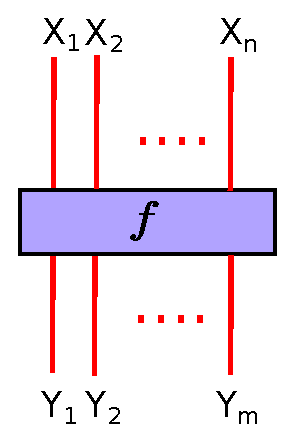
\includegraphics[width=0.15\textwidth]{morphnew.eps}
\end{center}
For morphisms $f:X\ra Y, g:Y\ra Z$, their composition $f\circ g: X\ra Z$ is denoted simply by stacking them.

\begin{center}
\includegraphics[width=0.04\textwidth]{morphism.eps}
\end{center}

For morphisms $f:X\ra Y, g:X'\ra Y'$, their tensor product $f\ot g: X\ot X' \ra Y \ot Y'$ is denoted as
\begin{center}
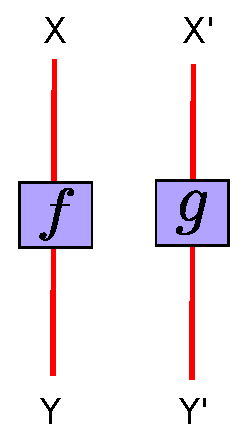
\includegraphics[width=0.1\textwidth]{tensor.eps}
\end{center}
The above rules easily generalize to cases when the source and/or target of a morphism consists of several tensor factors.
\subsection{Rigidity}
\begin{Def}
 A \textit{left rigid} structure on a monoidal category $\C$ is an endofunctor $*:\C \rightarrow \C, X\mapsto X^*$, with evaluation and coevaluation morphisms \begin{align}
	\coev: \one \rightarrow X\otimes X^*\quad, \quad \quad \ev:X^*\otimes X \rightarrow \one  
	,
\end{align}
\begin{center}
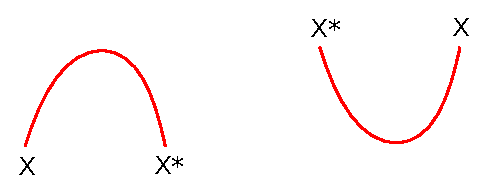
\includegraphics[width=0.4\textwidth]{duals.eps}
\end{center}
for each $X \in \C$ such that the following `snake diagrams' are satisfied,

\begin{center}
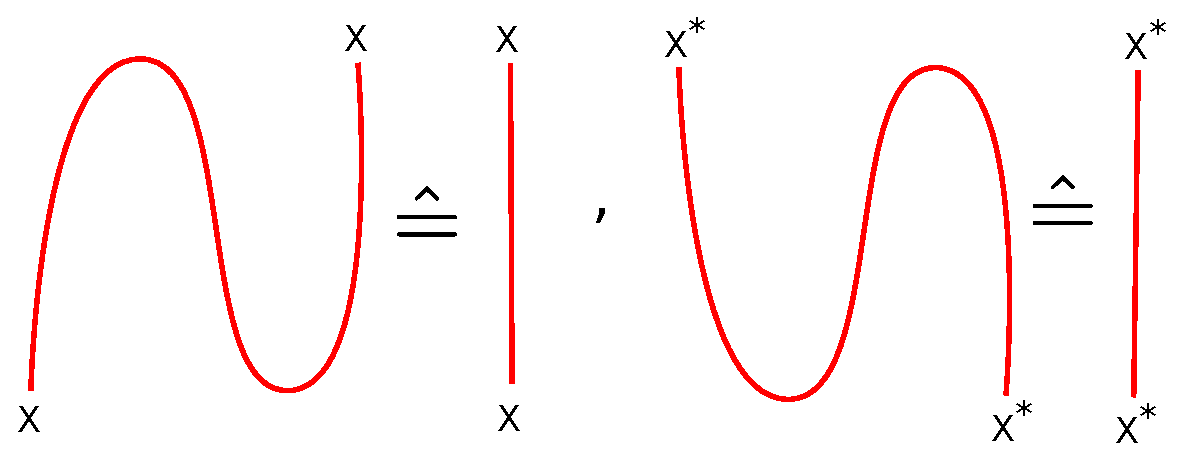
\includegraphics[width=0.6\textwidth]{snake.eps}
\end{center}
i.e., the following equations are satisfied, \begin{align}
	\label{rigid2}\id_X &= (\id_X \otimes \ev_X) \circ\alpha_{X, X^*, X}\circ(\coev_{X} \otimes \id_X),\\ \label{rigid1}\id_{X^*} &= (\ev_X\otimes \id_{X^*})\circ \alpha_{X^*, X,  X^*}\circ(\id_{X^*}\otimes \coev_X)
	.
\end{align}

\end{Def}

The object $X^*$ is called the \textit{left dual} of $X$. A \textit{right rigid} structure with a \textit{right dual} ${}^*X$ for each $X\in \C$ is defined similarly. The object $X$ is the right dual of $X^*$ and the left dual of ${}^*X$. Left (or right) duals are unique upto a unique isomorphism. Suppose an object $X$ has 2 left duals $X_1^*$ and $X_2^*$, then there is an isomorphism \begin{equation}
	X_1^* \xrightarrow{\id \otimes \coev_2} X_1^* \otimes (X\otimes X_2^*) \xrightarrow{a_{X_1^*, X, X_2^*}} (X_1^* \otimes X ) \otimes X_2^* \xrightarrow{\ev_1 \otimes \id} X_2^*.
\end{equation}\\

For a morphism $f:X\rightarrow Y$, its \textit{dual morphism} $f^*: Y^* \rightarrow X^*$ is defined as \begin{align}
	f^*:Y^*\xrightarrow{\id\otimes \coev_X} Y^* \otimes (X\otimes X^*) &\xrightarrow{a_{Y^*, X, X^*}} (Y^* \otimes X)\otimes X^* \nonumber \\ &\xrightarrow {(\id \otimes f) \otimes \id} (Y^* \otimes Y) \otimes X^* \xrightarrow{\ev_Y \otimes \id_{X^*}} X^*.
\end{align}
Graphically, $f^*$ is represented in terms of $f$ as the following diagram.
\begin{center}
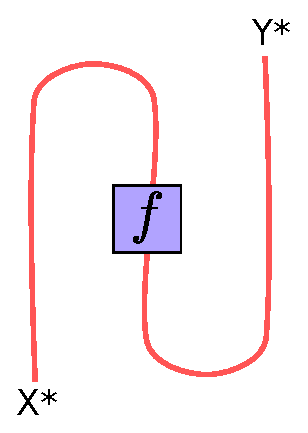
\includegraphics[width=0.15\textwidth]{fdual.eps}
\end{center}
\begin{Prop}
Given a tensor functor $F:\C \rightarrow \D$, with structure morphisms in $\D$, \begin{align}
	&J_{X,Y} : F(X) \otimes F(Y) \rightarrow F(X\otimes Y)\\
	&J_1 : \one \rightarrow F(\one),
\end{align}
and an object X with a left dual $X^*$, the object $F(X^*)$ is a left dual of $F(X)$ with evaluation and coevaluation maps given by
\begin{align}
	\ev_{F(X)}: F(X^*)\otimes F(X) \xrightarrow{J_{X^*, X}} F(X^*\otimes X) \xrightarrow{F(\ev_X)}F(\one) \xrightarrow{J_1} \one\\
	\coev_{F(X)}: \one \xrightarrow{J_0} F(\one) \xrightarrow{F(\coev_X)} F(X\otimes X^*) \xrightarrow{J_{X, X^*}} F(X) \otimes F(X^*).
\end{align}
\end{Prop}
\begin{proof}
Starting from the object $F(X^*)$, we have the composition 
\begin{align}
	(J_1\inv \otimes \id_{F(X^*)})\circ(F(\ev)\otimes \id_{F(X^*)})\circ (J\otimes \id_{F(X^*)}) \circ (\alpha_{F(X^*), F(X), F(X^*)})\circ \nonumber\\(\id \otimes J\inv_{X, X^*})\circ (\id_{FX^*}\otimes F(\coev))\circ (\id_{FX^*}\otimes J_1 )\\
	=(J_1\inv \otimes \id_{F(X^*)})\circ(F(\ev)\otimes F(\id_{X^*}))\circ J\inv_{X^*\otimes X, X}\circ F(\alpha_{X^*, X, X^*})\nonumber\\\circ (J_{FX^*, X\otimes X^*})\circ (F(\id_{X^*}) \otimes F(\coev))\circ (\id_{F(X^*)}\otimes J_1 )\\
	=(J_1\inv \otimes \id_{F(X^*)})\circ J\inv_{\one, X^*}\circ F(\ev \otimes \id_{(X^*)})\circ F(\alpha_{X^*, X, X^*})\nonumber\\\circ (J_{X^*, X\otimes X^*})\circ (F(\id_{X^*}) \otimes F(\coev))\circ (\id_{F(X^*)}\otimes J_1 )\\
	=(J_1\inv \otimes \id_{F(X^*)})\circ J\inv_{\one, X^*}\circ F(\ev \otimes \id_{(X^*)})\circ (F(\alpha_{X^*, X, X^*}))\nonumber\\\circ (F(\id_{X^*}\otimes\coev))\circ (J_{X^*, \one})\circ (\id_{F(X^*)}\otimes J_1 )\\
	=(J_1\inv \otimes \id_{F(X^*)})\circ J\inv_{\one, X^*}\circ(F(\ev \otimes \id_{(X^*)}))\circ (F(\alpha_{X^*, X, X^*}))\nonumber\\\circ (F(\id_{X^*}\otimes\coev))\circ (J_{X^*, \one})\circ (\id_{F(X^*)}\otimes J_1 )\label{last},
\end{align}
where we have used the fact that $F$ is a tensor functor and $J$ is a functorial isomorphism. In the last expression we can substitute,
\begin{align}
	F(\ev \otimes \id_{(X^*)})\circ F(\alpha_{X^*, X, X^*})\circ F(\id_{X^*}\otimes\coev)\nonumber\\ = F ((\ev \otimes \id_{(X^*)})\circ (\alpha_{X^*, X, X^*})\circ(\id_{X^*}\otimes\coev)) = F(\id_{X^*})  = \id_{F(X^*)},
\end{align}
and so the expression \ref{last} becomes \begin{align}
(J_1\inv \otimes \id_{F(X^*)})\circ J\inv_{\one, X^*}\circ (J_{X^*, \one})\circ (\id_{F(X^*)}\otimes J_1 )
\end{align}

which is the identity morphism as we have assumed the unit to be strict. A similar verification can be carried out for the object $F(X)$.
\end{proof}

\begin{Prop}
Let $U, V, W$ be objects having duals in a tensor category $\C$, and let $g: U\rightarrow V$, $ f:V\rightarrow W$ be morphisms in $\C$. Then $(f \circ g)^* = g^*\circ f^*$.
\end{Prop}
\begin{proof}
We prove this by graphical calculus,
\begin{center}
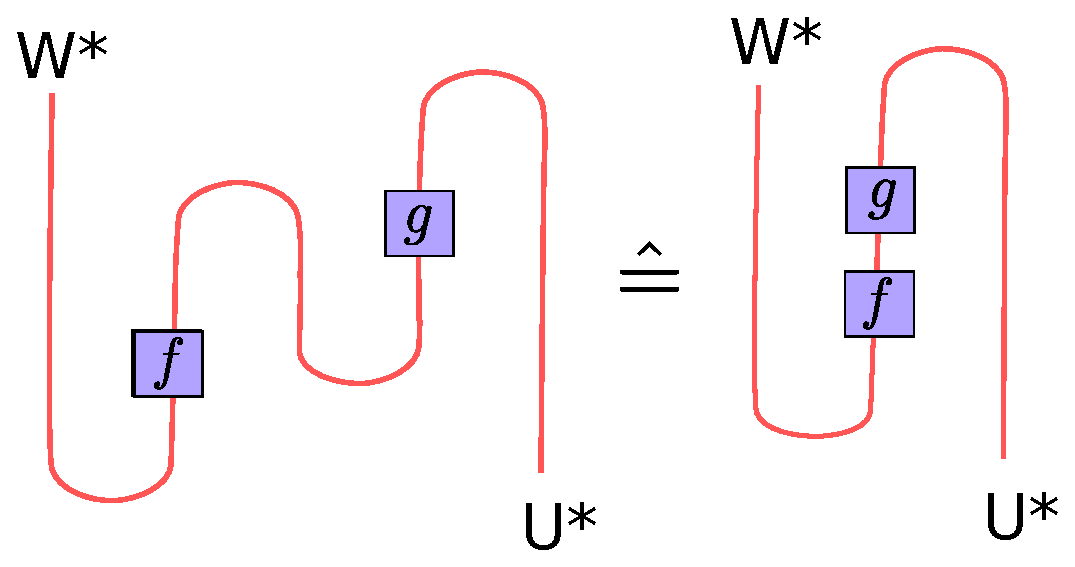
\includegraphics[width=0.5\textwidth]{dualcomposition.eps}
\end{center}
where we use equation (\ref{rigid2}) for the object $V^*$.
\iffalse
Consider the following map 
\begin{align}
\theta:  U \xrightarrow{g} V \xrightarrow{ \coev_V \ot \id_{V}}    (V \ot V^*) \ot V \nonumber\\\xrightarrow {\alpha_{V, V^*, V}} V\ot (V^*\ot V) \xrightarrow{\id_V \ot \ev_V} V \xrightarrow{f} W 
\end{align}
If $\Theta := \id_{W^*}\otimes \theta \otimes \id_{U^*}$, then the map \begin{align}
W^* \xrightarrow{\id_{W^*}\otimes \coev_U} W^* \otimes (U \otimes U^*)\xrightarrow{\alpha_{W^*, U, U^*}} (W^* \otimes U)\otimes U^* \nonumber\\\xrightarrow{\Theta } (W^*\otimes W) \otimes U^* \xrightarrow{\ev_W \otimes id_{U^*}} U^*\label{dualmor}
\end{align}
is by definition $g^*\circ f^*$. However, since $V^*$ is dual to $V$, the composition
\begin{equation}
	V \xrightarrow{ \coev_V \ot \id_{V}}    (V \ot V^*) \ot V \nonumber\\\xrightarrow {\alpha_{V, V^*, V}} V\ot (V^*\ot V) \xrightarrow{\id_V \ot \ev_V} V
\end{equation}
equals $\id_V$.
The map $\theta$ is then simply $f\circ g$ and the map \ref{dualmor} becomes $(f\circ g)^*$.
\fi
\end{proof}

\subsection{Fusion categories}
\begin{Def}
A locally finite semisimple rigid tensor category with a finite number of isomorphism classes of simple objects (which includes $\one$) is called a \textit{fusion category}.
\end{Def}
The rigid structure on arbitrary tensor categories can be quite complicated to understand but in the setting of fusion categories it behaves rather nicely.
\begin{Prop}
In a fusion category, any simple object $V$  is functorially isomorphic to its double dual $V^{**}$.
\end{Prop}
\begin{proof}
There are maps $V\otimes {}^*V\rightarrow \one$ and $\one \rightarrow V\otimes V^* $. Since the category is semisimple, there is an injection  $ \one \rightarrow V\otimes {}^*V$, and a projection $V\otimes V^*\rightarrow \one$, and so the left dual is isomorphic to the right dual, $V^*\cong {}^*V$, and hence $V\cong V^{**}$.
\end{proof}

Rigidity lets us define the notion of the trace of a morphism in a rigid monoidal category. For $V\in \C$, a rigid monoidal category,  $f\in \Hom(V, V^{**})$, the \textit{left trace}  is defined as \begin{align}
\tr_L(f): \one \overset{\coev_V}\longrightarrow V\otimes V^{*} \overset{f\otimes \id_V^*}\longrightarrow V^{**} \otimes V^* \overset{\ev_{V^*}}\longrightarrow \one \end{align} 
\begin{center}
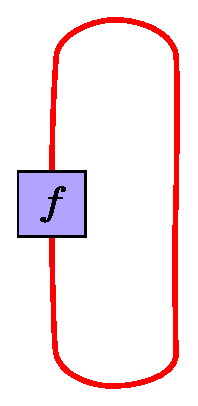
\includegraphics[width=0.08\textwidth]{lefttrace.eps}
\end{center}

Similarly, for $f: V^{**} \rightarrow V$, the \textit{right trace} is defined as
\begin{align}
\tr_R(f): \one \overset{\coev_{V^*}}\longrightarrow V^*\otimes V^{**} \overset{\id_{{}^*V}\otimes f}\longrightarrow V^* \otimes V \overset{\ev_{{}^{**}V}}\longrightarrow \one  
\end{align}
\begin{center}
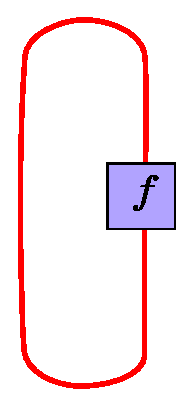
\includegraphics[width=0.08\textwidth]{righttrace.eps}
\end{center}

Let $f^* \in \Hom(V^{***}, V^*)$ be the dual morphism of $f\in \Hom(V, V^{**})$, then the right trace of $f^*$ is  \begin{equation}
	\tr_R(f^*): \one \overset{\coev_{V^{**}}}\longrightarrow V^{**}\otimes V^{***} \overset{ \id_{V^{**}} \otimes f^*}\longrightarrow V^{**} \otimes V^{*} \overset{\ev_{V}}\longrightarrow \one  
\end{equation}The left and right trace are related as $\tr_L(f) = \tr_R(f^*)$.

\subsubsection{Pivotality}
\begin{Def}
	A \textit{pivotal structure} on a rigid monoidal category is a monoidal functorial isomorphism from the double dual functor to the identity functor \begin{equation}
	j:  \id\rightarrow {}^{**} , \quad (\text{i.e.} \quad j_X :X\rightarrow X^{**}, \quad X\in \C ).
\end{equation}

\end{Def}Our primordial example $\Vect$, is an example of a pivotal category, where the pivotality is a result from elementary linear algebra, with the isomorphism $V\rightarrow V^{**}$ explicity described by \begin{equation}
	v\mapsto v' ,\quad  \text{such that} \quad v'(?) = ?(v)
\end{equation}  for $v\in V$, where $?$ stands for any element in $V^*$. An example of a category without a pivotal structure is the category $\Rep H$, the category of representations of a non-semisimple finite dimensional Hopf algebra (in fact, such a category has a functorial isomorphism from id to ${}^{****}$, the quadruple dual functor).
The following is an important open question in the theory of fusion categories. \begin{Conj}[Etingof-Nikshych-Ostrik]
Every fusion category admits a pivotal structure.
\end{Conj}
In a pivotal category, the pivotal structure on an object $X$, $j_X$ is related to the pivotal structure on its dual as \begin{equation}
	(j_X)^{*-1} = j_{X^*}
\end{equation} 

 Using the trace one can define for an object $V\in \C$, its quantum dimension \begin{equation}
	\dim V = \tr(\id_V)
\end{equation} 
In a pivotal fusion category $|V|^2 = \dim (V)\dim (V^*) = \dim (V)\dim (V^*)$, and so $|V|^2 = (\dim V)^2$. 
\begin{Def}
A fusion category is \textit{spherical} with respect to a given pivotal structure $j$, if $\tr_L(f) = \tr_R(f)$ for $f \in \End(X)$ where $X \in \C$.
\end{Def}

Let the above isomorphism be denoted $j_V:V\rightarrow V^{**}$. Define \begin{align}
	\tr_+(f) = \tr_L(j_V\circ f)\\
	\tr_-(f) = \tr_R(f\circ j_V\inv)
\end{align}
for a morphism $f: V\rightarrow V$.\\
Now let $\C$ be a fusion category. 
We can define the M\"uger's squared norm for a $X\in \OO(\C)$ given by \begin{equation}
	|X|^2 = \tr_+(\id_X)\tr_-(\id_X),
\end{equation}
and since $X$ is simple, $j_X$ is unique upto a scalar, rendering the above definition of the squared norm invariant under the choice of $j_X$. However, as [DSPS] note, the M\"uger squared norm is not canonically the square of anything. \\
\begin{Def}
The \textit{categorical} (or \textit{global}) \textit{dimension} of a fusion category is defined to be the sum of Muger's squared norms of its simple objects.
\end{Def}
\begin{Expl}\rm
Consider the category of finite dimensional representations of a finite group $G$, $\Rep(G)$.  The pivotal structure is inherited from $\Vect$, so the squared norm of an irreducible representation is the square of its vector space dimension. The categorical dimension of $\Rep(G)$ is \begin{equation}
	\sum_{V_i\in \OO(\Rep(G))} (\dim V_i)^2 = |G|.
\end{equation}
\end{Expl}
\begin{Def}
A \textit{fusion subcategory}  of a fusion category $\C$ is a full tensor subcategory $\C'\subset \C$ such that if $X\in \C$ is isomorphic to a direct summand of an object in $\C'$ then $X\in \C'$.
\end{Def}
 It is known that every fusion subcategory of a fusion category is rigid \cite[Corollary F.7]{MR2609644}.
 \begin{Def}
 The \textit{adjoint subcategory} of a fusion category $\C$ is the fusion subcategory $\C_{ad} \subset \C$ generated by objects of the form $X\otimes X^*$, for $X\in \OO(\C)$.
 \end{Def}
\begin{Def}
A \textit{grading} on a fusion category $\C$ by a group $G$ is a map \begin{equation}
	\text{deg}: \OO(\C) \rightarrow G \label{deg}
\end{equation}
such that if $Z\subset X\otimes Y$ then $\text{deg } Z = \text{deg } X\cdot \text{deg } Y$. A grading is \textit{faithful} if deg is surjective. 
\end{Def}

The grading yields a decomposition $\C = \bigoplus_{g\in G}\C_g$, where $\C_g$ is generated by simple objects of degree $g\in G$. The term grading is also used to refer to this decomposition. By the multiplicativity of the map deg, it is easy to see that $\C_{ad}\subset \C_1$ for any $G$.
\begin{Def}
There exists a \textit{universal grading group} $U_\C$ for any fusion category $\C$ such that for a faithful grading by any other group $G$, there is a surjective morphism $U_{\C}\rightarrow G$.
\end{Def}
\begin{Expl}\rm\label{VecOmegaG}
A class of fusion categories most relevant to this thesis are of the form $\Vect^\omega_G$, where $G$ is a finite group and $\omega$ is a 3-cocycle with values in $\CC^\times$. The simple objects of $\Vect^\omega_G$ upto isomorphism are of the form $V_g$ for $g\in G$. The tensor product is defined as \begin{equation}
	V_g\ot V_h \subseteq V_{gh},
\end{equation} with the associator $\omega$ given by \begin{equation}
	\omega(g, h, k): (V_g \ot V_h)\ot V_k \ra V_g \ot (V_h\ot V_k).
\end{equation}
All simples objects have dimension 1 and the categorical dimension of $\Vect_G$ is consequently $|G|$. It has a canonical pivotal structure since all its objects are vector spaces, and this pivotal structure is spherical. Its universal grading group is $G$. 
\end{Expl}
\iffalse
The following is an interesting result.
\begin{Prop}
Let $\C$ be a fusion category and let $G = U_{\C}$ be its universal grading group, and let $G_{ab} = G/[G, G]$ be the maximal abelian quotient of $G$. Then there is an isomorphism, \begin{equation}
	\widehat{G_{ab}} \xrightarrow{~} \Aut_{\otimes}(\id_\C),
\end{equation}
where $G_{ab}$ denotes the group of characters of $G_{ab}$.
\end{Prop}
\begin{proof}
Define a grading on $\C$ by $G$ given by \begin{equation}
	\C_\chi = \{X\in \C \text{ }|\text{ } \Phi_X = \chi(\Phi)\id_X\}
\end{equation}
where $\chi \in  \widehat{\Aut_{\otimes}(\id_\C)}$. Since $G$ is the universal grading group, any faithful grading by an abelian group factors through $G_{ab}$. Hence there is a surjective morphism $G_{ab}\rightarrow \widehat{\Aut_{\otimes}(\id_\C)}$. 
Now let  $\pi:G\rightarrow G_{ab}$ denote the quotient map, and let $\C = \bigoplus_{x\in G_{ab}}\C_x$ be the grading of $\C$ by $G_{ab}$, where two objects of degree $x,y \in G$ respectively, belong to the same component of the grading if and only if $\pi(x) = \pi(y)$. Now let $\Phi_\chi\in \Aut_{\otimes}(\id_\C)$ be defined as \begin{equation}
	(\Phi_\chi)_X = \chi(a)\id_X
\end{equation} for $X \in \C_a$. There is an injective group homomorphism $\chi\rightarrow \Phi_\chi$, which establishes the desired isomorphism.                    
\end{proof}
\fi


\subsection{Pointed fusion categories}\label{pfc}
Perhaps the simplest examples of fusion categories are the so-called \textit{pointed fusion categories}, whose simple objects are all invertible with respect to the tensor product operation, i.e., for every simple object $X$, there is a simple object $Y$ such that \begin{equation}
	X\otimes Y \cong \one, \quad Y\otimes X\cong \one.
\end{equation}
In other words, they are fusion categories such that $\C_{ad}$ is generated by $\one$. 
Objects in  $\OO(\D)$, under the $\ot$ operation, form a group $G$ which induces a grading on $\D$ by $G$, with each homogeneous component generated by an element of $\OO(\D)$. We have an isomorphism between the fusion rings of $\D$ and $\Vect^\omega_G$,  \begin{equation}
	\OO (\D) \rightarrow G \quad X\mapsto g. \label{pointedrings}
\end{equation} which is simply the deg map from \eqref{deg}. Since all objects in $\Vect_G^\omega$ have dimension 1, by the isomorphism of fusion rings (\ref{pointedrings}), so do all objects of $\D$.
Define the associator on a triple of simple objects\begin{equation}
	\omega(g,h,k):(X_g \otimes X_h) \otimes X_k \rightarrow    X_g \otimes (X_h\otimes X_k)
\end{equation} for $X_g \in \OO(\D)$. 
 Each $\omega(g,h,k)$ is an isomorphism between 1-dimensional vector spaces, and is given by an element of $\GL_1(\kk) = \kk^\times$.  The fact that $\omega$ must satisfy the pentagon axiom leads to the condition \begin{equation}
	\omega(g,h, kl)\omega(gh, k, l) = \omega(h,k,l)\omega(g, hk, l)\omega(g,h,k).
\end{equation} This is exactly the condition for a 3-cocycle, so $\omega \in Z^3(G, \CC^\times)$.  A similar argument for the unit axioms gives the condition that $\omega$ is a normalized 3-cocycle, which means $\omega(g, h, k)=1$ if either $g, h$ or $k$ is 1. One can establish a tensor equivalence \begin{equation}
	F: \D \rightarrow \Vect^\omega_G,
\end{equation} using the natural transformation $\eta_{X_g,X_h}: F(X_g)\otimes F(X_h) \rightarrow F(X_g\otimes X_h)$ which is explicity given by a function $\eta:G\times G \rightarrow \kk^\times$. Using the hexagon axiom for a tensor functor and the fact that $F(X_1) = \one$, we get the condition that $d\eta$ is a normalized 2-coboundary. The quasi-inverse of $F$ is defined similarly with the help of the function $\eta\inv$. We have thus shown that any pointed fusion category is equivalent to $\Vect^\omega_G$ where $\omega$ is a 3-cocycle and $G$ is a finite group. The fact that $d\eta$ is a normalized 2-coboundary implies that if $\Vect^\omega_G$ and $\Vect^{\omega'}_G$ are such that $\omega $ and $\omega'$ are cohomologous, then the two categories are tensor equivalent.


\section{Module categories and categorical Morita equivalence}\label{section:module-categories}
\begin{Def}\rm\label{modulecategorydef}
For $\C$ a fusion category, a left $\C$-module category $\M$ over a fusion category $\C$ is a semisimple locally finite category $\M$ with a finite number of simple objects,  together with a bilinear functor $\otimes^{\M}: \C\times \M\ra \M$ along with natural isomorphisms \begin{align}
	\beta &: \otimes^{\M} \circ (\otimes ^{\C} \times \id_{\M})\cong  \otimes^{\M} \circ (\id_{\C} \times \otimes^{\M})\\
	l^\M &: (\one \otimes^{\M} - ) \cong \id_{-}
\end{align}
satisfying the pentagon and triangle identities for object $X, Y, Z \in \C$ and $M\in \M$.
\[
  \xymatrix{&  X\otimes^\M (Y\otimes^\M (Z \otimes^\M M)) & \\ 
  X\otimes^\M ((Y\otimes^\C Z) \otimes^\M M) \ar[ru]^{\id_X \otimes^\M (\beta_{Y, Z, M})} &  & (X\otimes^\C Y)\otimes^\M (Z \otimes^\M M))\ar[lu]^{\beta_{X, Y, Z\otimes^\M M}}\\ 
  (X\otimes^\C (Y\otimes^\C Z)) \otimes^\M M \ar[u]_{\beta_{X, Y\otimes Z, M}} &  &  \ar[ll]^{\alpha_{X, Y, Z}\otimes^\M M} ((X\otimes^\C Y)\otimes^\C Z) \otimes^\M M\ar[u]^{\beta_{X\otimes Y, Z, M}} }
\]
\[
\xymatrix{(X\otimes^\C \one) \otimes^\M M \ar[rr]^{\beta_{X, \one, M}}\ar[dr]^{r_X} && X\otimes^\M(\one \otimes^\M M)\ar[dl]^{l^\M_M}\\
& X\otimes M }
\]
\end{Def}

Alternatively, it can also be defined as a semisimple locally finite category $\M$ with a finite number of simple objects, carrying the additional data of a $\kk$-linear monoidal functor $F:\C\rightarrow \End(\M)$, where $\End(\M)$ denotes the category of $\kk$-linear endofunctors of $\M$, where the tensor product structure is given by composition.
\begin{Prop}
The two definitions of a $\C$-module category given above are equivalent.
\end{Prop}
\begin{proof}
Let $F:\C\rightarrow \End(\M)$ be the functor defining the structure of a $\C$-module category on $\M$ from the second definition. One can define the module category structure $\otimes^{\M}$ as \begin{equation}
	X\otimes^{\M} M := F(X)(M)
\end{equation}
The isomorphism $(X\otimes^\C Y)\otimes^\M M\rightarrow X\otimes^\M (Y\otimes^\M M)$ for $X, Y \in \C$ is given by \begin{equation}\label{moddef2}
	(X\otimes^\C Y)\otimes^\M M := F(X\otimes Y)(M) \xrightarrow{J\inv_{X, Y}(M)} F(X)\circ F(Y)(M) =: X\otimes ^\M (Y\otimes^\M M )   
\end{equation}
In the other direction, If $\M$ is a $\C$-module category, then for $X\in \C$, \begin{equation}
	M\rightarrow X\otimes^\M M
\end{equation}
defines an endofunctor of $\M$, with the monoidal structure defined using the associativity constraint $m_{X, Y, M}$.
\begin{equation}\label{moddef1}
	F(X)\circ F(Y)(M):= X\otimes^\M (Y \otimes^\M M) \xrightarrow{m\inv_{X, Y, M}} (X\otimes^\C Y) \otimes^\M M=: F(X\otimes^\C Y) \otimes^\M M 
\end{equation} It is straighforward to verify the pentagon and triangle axioms for both the definitions (\ref{moddef2}) and (\ref{moddef1}).
\end{proof}
Similar definitions can be written down for a right $\C$-module category, and also for a $\C-\D$-bimodule category, where $\D$ is also a fusion category. From now on we will stop labeling the tensor product with the respective category, banking on the fact that this will be clear from context.	
\begin{Expl}\rm
Every finite category is a $\Vect-\Vect$-bimodule category in a unique way. Let $X\in \C$ and $V \in \Vect$, then $V\cong \kk^n$ for some positive integer $n$, and so the left module structure is given by the composition\begin{equation}
	V\otimes X \mapsto \kk^n \otimes X \mapsto X^{\otimes n},
\end{equation} and similarly for the right module structure. Since the resulting bimodule structure only depends on the identification of $V$ with $\kk^n$ (which is unique upto a unique natural isomorphism), any such structure is unique upto a unique natural isomorphism. 
\end{Expl}
\begin{Expl}\rm
Any fusion category $\C$ is itself naturally a $\C-\C$-bimodule category, or equivalently a left $\C \boxtimes \C^{op}$ module category, where $\boxtimes$ denotes the Deligne tensor product. 
\end{Expl}
\begin{Expl}\rm
For $G$ a finite group, $\Vect$ is a right $\Rep(G)$-module category, where an object $V\in \Rep(G)$ acts by $F(V)\otimes -$, where $F:\Rep(G)\rightarrow \Vect$ denotes the forgetful functor. 
\end{Expl}
\begin{Expl}\rm
For any algebra object $A$ in a fusion category  $\C$, the category $\Mod_C-A$ of right $A$-modules in $\C$ is a left $\C$-module category, for details see Theorem \ref{Ostrik}.
\end{Expl}
\begin{Def}
A $\C$-module functor $F:\M\rightarrow \NN$ is a functor $F:\M\rightarrow \NN$ along with a functorial isomorphism \begin{equation}
	s_{X, M}: F(X\otimes M) \rightarrow X\otimes F(M)  
\end{equation} for $X\in \C$ and $M\in \M$, such that the following diagrams commute. 
\[
\xymatrix{
& F((X\ot Y) \ot M) \ar[rd]^{F(m_{X, Y, M})} \ar[ld]^{s_{X\ot Y, M}}& \\
(X\ot Y) \ot F(M) \ar[d]^{m'_{X, Y, F(M)}} & &  F(X \ot (Y\ot M))\ar[d]^{s_{X, Y\ot M}} & \\
X\ot (Y \ot F(M))& & X \ot F(Y\ot M)\ar[ll]^{s_{Y, M}} }
\]
\[
\xymatrix{F(\one\ot M) \ar[rr]^{s_{\one, M}} \ar[rd]^{F(l_M)}& &  \one \ot F(M)\ar[ld]^{l_{F(M)}}\\
& F(M) & }
\]
\end{Def}
\begin{Def}
A \textit{ $\C$-module functorial morphism} $\nu$ between functors $(F,m)$ and $(G, n)$ is a functorial morphism $\nu:F\rightarrow G$ that is natural with respect to the module functor structure, i.e., \[
	\xymatrix{
  	F(X\otimes M) \ar[d]_{\nu_{X\otimes M}}\ar[r]^{s_{X, M}} & X\otimes F(M)\ar[d]^{\nu_X \otimes \id_M}\\
   G(X\otimes M)	 \ar[r]^{s'_{X, M}} & X\otimes G(M).}			
\]

\end{Def}
$\C$-module functors between $\C$-module categories $\M$ and $\NN$ form a category, with morphisms being $\C$-module functorial morphisms.

We will now discuss the module categories over $\Vect^\omega_G$ which are relevant to this thesis. A module category over $\Vect^\omega_G$ is an abelian category with the auto-equivalences $F_g:M\rightarrow \delta_g \otimes M$ and a monoidal functorial isomorphism $\eta$, \begin{equation}
	\xymatrix{F_g\circ F_h (M) \ar[r]^{\eta_{g,h}^M}\ar[d]_{F_g\circ F_h(f)} & F_{gh}(M) \ar[d]^{F_{gh}(f)} \\
	F_g\circ F_h(N) \ar[r]^{\eta_{g,h}^N} & F_{gh}(N)} 
\end{equation} for $g,h \in G$, objects $M, N \in \M$ and $f\in \Hom(M, N)$. Since the multiplication in $G$ is associative, the monoidal functorial isomorphisms $\eta$ obey the 2-cocycle relation.

\begin{equation}
	\eta(g, h)\eta(gh,k) = \eta(h,k)\eta(g, hk)
\end{equation}

A simple object $M$ in an indecomposable semisimple category $\mathcal{M}$ over $\Vect^\omega_G$ has an action of a simple object $\delta_g\in \Vect^\omega_G$, such that $\delta_g \otimes M$ is also a simple object (suppose on the contrary that it decomposes as a direct sum, then by acting with $\delta_{g\inv}$ we get a decomposition for $M$). Since $\M$ is indecomposable this action of $G$ must be transitive, for if this wasn't the case, then each orbit of $G$ would be an indecomposable category and $\M$ would decompose as a Deligne product of these. By the orbit-stabilizer theorem, the simples are a transitive $G$-set, where the stabilizer $L$ is unique upto an inner automorphism of $G$.  For the trivial $L$-module $\kk^\times$, we define
\begin{equation}
	\Coind^G_L \kk^\times := \Hom_L(G,\kk^\times)\simeq \text{Fn}(G/L, \kk^\times),
\end{equation}
i.e., functions from $G/L$ to $\kk^\times$. It has a left $G$-module structure,  $g\cdot f(x) = f(g\inv x)$ for an $L$-linear $f:G\rightarrow \kk^\times$.
The associator  $\alpha_\M (\delta_g,\delta_h,M): (\delta_g\ot \delta_h)\ot M\rightarrow \delta_g\ot (\delta_h\ot M)$  is given by a function $m:G\times G \times G/L\rightarrow \kk^\times,$ where $M$ corresponds to the class $[b]\in G/L$, such that
\begin{equation}\label{pent}
	\omega(g,h,k)m(g, hk, b)m(h, k, b) = m(gh, k, b)m(g, h, kb)
\end{equation}

Define $\Psi: G\times G \rightarrow \Coind^G_L k^\times$, 
\begin{align}
	\Psi(g,h)(b) &= m(g, h, h\inv g\inv b) \\
	\Psi(g,h)(ghb) &=  m(g, h, b)\\
	(gh)\inv\cdot\Psi (g,h)(b) &= m(g,h,b)
\end{align}
Using equation (\ref{pent}) with trivial $\omega$,
\begin{align}
	(ghk)\inv\cdot \Psi(g, hk)(b)(ghk)\inv g\cdot \Psi(h, k)( b) &=  (ghk)\inv\cdot \Psi(gh, k)( b)(ghk)\inv \cdot \Psi(g, h)(b)\\
 \Psi(g, hk)g\cdot \Psi(h, k) &=   \Psi(gh, k) \Psi(g, h)
\end{align}
which is the desired cocycle condition on $\Psi$. For a $\Vect^\omega_G$-module functor $F:\M\ra \NN$, the structure isomorphisms \begin{equation}
	s_{\delta_g, M}: F(\delta_g \ot M)\ra \delta_g\ot F(M)
\end{equation} are given by a function $G\ra \text{Fn} (G/L, \kk^\times)$, denoted by $\xi(g)$ for $g\in G$. In case of an equivalence $F$ of module categories, the pentagon axiom gives the condition \begin{equation}
	F(\Psi(g, h))  = \Psi'(g, h) \xi(g)\xi(h)\xi(gh)\inv.
\end{equation} We see that the equivalence class of $\Psi$ depends on $H^2(G, \Coind^G_L k^\times)$.\\
 \begin{Lem}[Shapiro's lemma]For a ring morphism $f:R\rightarrow S$, such that $S$ is a projective right $R$-module, and if $M$ and $N$ are right $S$ and $R$ modules respectively, then 
 \begin{equation}
  	\Ext_S^n(M, \Coind N) \simeq \Ext_R^n (\Res M, N).
  \end{equation} 
 
 \end{Lem}
For the morphism $L\rightarrow G$, with $N=k^\times$ and $M=G$, for $n=1$ we have the isomorphism
\begin{align*}
 	H^2(G, \Coind^G_L k^\times) &\overset{\sim}\longrightarrow H^2(L, k^\times)\\
 	\Psi &\mapsto \psi.
 \end{align*} 
 $F$ induces a map of $G$-sets, and following the above discussion $F(\psi(g, h)) = \psi(x\hit g, x\hit h) =: \psi^x(g, h)$ for some element $x\in G$.
\begin{theorem}\label{simpleparam}
A semisimple indecomposable $\Vect^\omega_G$ module category is determined by ($L,\psi$), where $L$ is a subgroup of $G$ and $\psi$ is a 2-cocycle.
\end{theorem}
We can conclude from the foregoing discussion that two pairs $(L, \psi)$ and $(L', \psi')$ correspond to equivalent module categories if and only if $L' = g\hit L$ and $\psi^g$ is cohomologous to $\psi'$.


\subsection{Algebra objects in fusion categories and Ostrik's theorem}
Let $\C$ be a fusion category.
\begin{Def}\label{algdef}
 An algebra object $(A, \nabla, u)$ is an object $A\in \C$ together with morphisms $\nabla:A\otimes A \rightarrow A$  and $u: \one\rightarrow A$ such that the following diagrams commute.
\[
\xymatrix{(A \otimes A) \otimes A \ar[d]_{\nabla \otimes \id_A} \ar[rr]^{\alpha_{A, A, A}}& & A\ot (A\ot A)\ar[d]^{\id_A\otimes \nabla}\\
A\otimes A \ar[rd]_{\nabla} & & A\otimes A\ar[ld]^{\nabla}\\
& A & }
\]
\[
\xymatrix{ \one \ot A\ar[d]^{u\ot \id_A} \ar[r]^{l_A} & A\ar[d]^{\id_A} \\
A\ot A \ar[r]^{\nabla} & A
}
\xymatrix{  A\ot \one \ar[d]^{ \id_A\ot u} \ar[r]^{r_A} & A\ar[d]^{\id_A} \\
A\ot A \ar[r]^{\nabla} & A
}
\]
\end{Def}

\begin{Expl}\rm
In any fusion category, the unit object $\one$ is naturally an algebra object.
\end{Expl}

\begin{Expl}\rm
In a pointed fusion category $\Vect^\omega_G$, consider the couple $(H, \mu)$ parametrizing the object $\CC_\mu H$, where $H$ is a subgroup of $G$. and $\mu \in Z^2(H, \CC^\times)$. By a slightly more general form of Lemma (\ref{simpleparam}), this is an algebra object if the diagram in  Definition \ref{algdef} commutes.  The commutativity of the above diagram gives us the condition that \begin{equation}
	\omega|_{H^3} = d\mu.
\end{equation} Hence, algebra objects in $\Vect^\omega_G$ are paramatrized by $(H, \mu)$, where $H$ is a subgroup of $G$ and $\mu$ is a 2-cocycle obeying the above condition.
\end{Expl}
\begin{Expl}\rm\label{canonicalalg}
Objects of the form $X\otimes X^*$ for $X\in \C$, a fusion category, are algebra objects, with multiplication $\nabla = \id_X \otimes \ev_X \otimes \id_{X^*}$, and $u = \coev_X$. Recall that these are the objects that generate the adjoint subcategory $\C_{ad}$.
\end{Expl}

\begin{Def}
A right $(A, \nabla, u)$-module  $(M, p) \in \C$ is an object $M\in \C$ with the structure map $p: M \ot A\rightarrow M$ which is associative in the category, i.e., the following diagram commutes. \[
\xymatrix{
	(M \ot A)\ot A \ar[rr]^{\alpha_{M,A,A} } \ar[d]^{\nabla \ot \id_M} & &  M\ot (A \ot A)  \ar[d]^{\id_A \ot p}\\
	 M\ot A \ar[r]^p& M &  M\ot A\ar[l]_p
}
\]
\end{Def}
From now on we will drop the structure maps while denoting algebras or modules and invoke them wherever necessary. 
\begin{Rem}\label{leftmod}
For a right $A$-module $M$, the object ${}^*M$ has the structure of a left $A$-module, given by the image of $p$ under the isomorphisms \begin{equation}
	\Hom(M\ot A, M)\cong \Hom({}^*M, ({}^*M\ot {}^*A)) \cong \Hom({}^*M, {}^*A \ot {}^*M) \cong \Hom(A\ot {}^*M, {}^*M).
\end{equation}
\end{Rem}
Given $A$-modules $M_1,M_2\in \C$, The space of $A$-module morphisms $\Hom_A(M_1, M_2)$ is a subspace of $\C(M_1, M_2)$, and thus we may talk about the $\kk$-linear category $\Mod_\C(A)$. 
\begin{Prop}\label{modcasemisimple}
  $\Mod_\C(A)$ is a semisimple category.
 \end{Prop}
 \begin{proof}
 We will show that every object $M \in \Mod_\C(A)$ is projective. We use the fact that if $A$ is a semisimple algebra over $k$, then the product map $\nabla: A\otimes A \rightarrow A$ splits as a map of $A$-bimodules. Then $M = M\otimes_A A$ is a direct summand of $M\otimes_A A\otimes A= M\otimes A$. Now, the functor \begin{equation}
 	\Hom_A(M \otimes A, -) \cong \C(M, \Forg(-))
 \end{equation}
 is exact because $M$ is a projective object in $\C$. Hence $M\otimes A$ is projective, and consequently so is $M$.
 \end{proof}
 For an object $X \in \C$ and an $A$-module $M\in \C$, the object $X\otimes M$ has a canonical structure of a right $A$-module, given by the following composition \begin{equation}
	p_{X\otimes M}: (X\otimes M) \otimes A  \xrightarrow{\alpha\inv_{X, M, A}} X\otimes (M \otimes A) \xrightarrow{\id_X \otimes p} X\otimes M.
\end{equation}
In fact, this map is nice enough to be extended to a left $\C$-module structure on $\Mod_\C(A)$, \begin{equation}
	\C \otimes \Mod_\C(A) \rightarrow \Mod_\C(A).
\end{equation}
We need to finally check that \begin{equation}
	(X\otimes Y) \otimes M \cong X\ot (Y\otimes M) 
\end{equation} is an $A$-module morphism.

\[
\xymatrix{((X\otimes Y ) \ot M)\ot A \ar[rr]^{\alpha_{X, Y, M} \ot A} \ar[d]^{\alpha_{X\ot Y, M , A}} & & (X\otimes(Y\ot M)) \ot A \ar[d]^{\alpha_{X, Y\ot M, A}}\\
(X\ot Y) \ot (M\ot A)\ar[dd]_{(X\ot Y)\ot m)} \ar[rrd]^{\alpha_{X, Y, M\ot A}}&  & X\ot ((Y \ot M) \ot A) \ar[d]^{X\ot \alpha_{Y, M, A}}\\
& & X\ot(Y\ot(M\ot A)) \ar[d]^{X\ot(Y\ot m)}\\
X\ot (Y\ot M) \ar[rr] & & (X\ot Y)\ot M
}
\]
The top pentagon commutes because $\alpha$ is an associator, and the bottom square commutes because $\alpha$ is tensor functorial in $\C$.
\begin{Lem}
For the algebra object $A=X\ot X^*$, $X^*\ot_A X\cong \kk$.
\end{Lem}
\begin{proof}
We want to show that \begin{equation}
	X^*\ot X \ot X^* \ot X \ot X^* \rightrightarrows X^*\ot X \ra \kk
\end{equation} is a coequalizer. We will use the universal property of the tensor product to prove this. Consider a map \begin{equation}
	f: X^* \ot_A X \ra V
\end{equation} for some object $V$. This means there's a map $g:X^*\ot X\ra V$ such that \begin{equation}
X^*\ot X \ot X^* \ot X 	\rightrightarrows V,
\end{equation} where the maps $\ev_X \ot g$ and $g \ot \ev_X$ should agree on $V$. Let $K=\ker (\ev)$, then $K\ot X^*\ot X + X^*\ot X \ot K$ lies in the kernel of $\ev_X\ot g = g\ot \ev_X$. Now for the exact sequences \begin{align*}
	0\ra K \ra X^*\ot X \ra \kk \ra 0\\
	0\ra K \ra X^*\ot X \ra \kk \ra 0,
\end{align*} the map $X^*\ot X \ot X^*\ot X \ra \kk$ also has kernel $K\ot X^*\ot X + X^*\ot X \ot K$, so the map $f$ factors through $\kk$, and thus we have the claimed isomorphism.
\end{proof}
\begin{Rem}\label{Cmoduleeqv}
For an object $X\in\C$ and $A=X\ot X^*$ we may establish an equivalence of $\C$-module categories \begin{align}
\C&\ra \Mod_\C(A)\\
Y&\mapsto Y\ot X^*\\
M\ot_A X&\mapsfrom M.
\end{align}
\end{Rem}
\begin{Def}
An algebra $A$ is \textit{semisimple} if $\Mod_\C(A)$ is semisimple. It is \textit{indecomposable} if $\Mod_\C(A)$ cannot be written as a Deligne product of module categories. 
\end{Def}
Using the observation in Proposition \ref{modcasemisimple}, one is tempted to make the following claim. \begin{theorem}[Ostrik]\label{Ostrik}
Every indecomposable left $\C$-module category is equivalent to a category $\Mod_\C(A)$ for a semisimple indecomposable algebra object $A\in\C$.
\end{theorem}
Before we prove this theorem, we need to define the internal Hom. 
Consider the functor \begin{equation}
	\M(-\otimes M, N): \C\rightarrow \Vect, X\mapsto \M(X\otimes M, N) 
\end{equation} for a fixed $M, N\in \M$.
Since every object in $\M$ is projective, this functor is exact and is hence representable. The representing object for this functor $\underline{\Hom}(M, N)$ is called the \textit{internal Hom} between $M$ and $N$. There is a natural isomorphism \begin{equation}
	\M(X\otimes M, N) \cong \C(X, \underline{\Hom}(M, N)).\label{internalhomiso}
\end{equation}
\begin{Lem}
 The bifunctor, \begin{align}
 \underline{\Hom} (?, -) : \M\times \M &\rightarrow \C\\
	(M, N) &\rightarrow \underline{\Hom}(M, N)
\end{align} is exact in both variables.
 \end{Lem} 
 \begin{proof}
 Consider an exact sequence \begin{equation}\label{internalhomseq}
	0\ra X\ra Y \ra Z \ra 0,
\end{equation}and let us apply the functor  $\C(A\ot W, -)$ for $A\in \C$ and $W\in \M$,
\begin{equation}
	0 \ra \C(A\ot W, X)\ra \C(A\ot W, Y) \ra \C(A\ot W, Z)\ra 0.
\end{equation}
This functor is exact because $\M$ is semisimple. Using the definition of the internal Hom, we now have, \begin{equation}
	0 \ra  \C(A,\underline{\Hom} (W, X))\ra \C(A,\underline{\Hom} (W, Y)) \ra \C(A,\underline{\Hom}(W, Z))\ra 0.
\end{equation}
Since $A\in \C$ is a projective object it follows that \begin{equation}
	0 \ra \underline{\Hom} (W, X) \ra \underline{\Hom} (W, Y) \ra \underline{\Hom}(W, Z)\ra 0,
\end{equation}
which proves exactness in the second variable.
Exactness in the first variable can be proved by applying the functor $A\ot -$ to the sequence \ref{internalhomseq} followed by $\C(-, W)$, and proceeding similarly. Both these functors are again exact because $\C$ and $\M$ are semisimple.
 \end{proof}
The object $\underline{\Hom} (M, M)\in \C$ for some $M\in\M$, has the structure of an algebra object in $\C$. Consider the map \begin{equation}
	\ev_M: \underline{\Hom} (M, M) \otimes M \rightarrow M
\end{equation} where the action of $\underline{\Hom} (M, M)$ is given by the $\C$-module structure. Hence, the multiplication \begin{equation}
\nabla_M:	\underline{\Hom} (M, M)\otimes \underline{\Hom} (M, M) \rightarrow \underline{\Hom} (M, M)
\end{equation} is given by composition. We also have the canonical unit morphism \begin{equation}
	\one\rightarrow \underline{\Hom}(M,M),                                                  
\end{equation}which is the image of $\id_M\in \Hom_\M(M, M)$ under equation \ref{internalhomiso}, with $X=\one$. 
The multiplication is associative since composition is associative. 
In addition, the internal Hom has the following property.
\begin{Lem}\label{internalhomlemma}
For objects $X,\in \C$, $ M, N\in \M$,
\begin{equation}
\underline{\Hom}(M, X\otimes N) \cong X \otimes \underline{\Hom}(M, N).
\end{equation}
\end{Lem}
\begin{proof}
Let $Y$ be an object in $\C$, then using the definition of the internal Hom and the the Hom-tensor adjunction, \begin{align}
	\C(Y, \underline{\Hom}(M, X\ot N)) \cong \M(Y\ot M,  X\ot N) \cong \M(X^* \ot (Y\ot M),  N) \\
	\cong \M((X^* \ot Y)\ot M,  N) \cong \C(X^* \ot Y, \underline{\Hom}( M,  N)) \cong \C(Y, X\ot \underline{\Hom}(M,  N)).
\end{align} 
\end{proof}

\begin{proof} [Proof of Theorem \ref{Ostrik}]
Let $A=\underline{\Hom} (M,M)$ for $M\in \M$. Consider the following adjunction \begin{equation}
	- \otimes_A M : \Mod_\C(A) \leftrightarrows  \M : \underline{\Hom}( M, -) 
\end{equation}is an equivalence. First, for any object $X\in \Mod_\C(A)$, we need to show that \begin{equation}
	\underline{\Hom}(M, X\otimes_A M) \cong X
\end{equation}
Using the property from Lemma \ref{internalhomlemma} and the fact that the internal Hom is exact in both variables, we can construct the following diagram \begin{equation}\label{coequalizercommute}
	\xymatrix{\underline{\Hom}(M, X\otimes A \otimes M) \ar@<-.5ex>[r] \ar@<.5ex>[r]\ar[d]^{\sim} & \underline{\Hom}(M, X\otimes M) \ar[r]\ar[d]^{\sim} & \underline{\Hom}(M, X\otimes_A M)\ar@{-->}[d] \\
	X\otimes A \otimes \underline{\Hom}(M, M) \ar@<-.5ex>[r] \ar@<.5ex>[r] & X\otimes \underline{\Hom}(M,  M) \ar[r] & X\otimes_A \underline{\Hom}(M,  M)\cong X.}
\end{equation} which commutes because the coequalizer is unique upto a unique isomorphism.

In the other direction, for every $Y \in \M$, we must show\begin{equation}
	 \underline{\Hom} (M,Y) \otimes_A M \cong Y.
\end{equation}
We have the following series of isomorphisms \begin{equation}
	\underline{\Hom}(M, \underline{\Hom} (M,Y) \otimes_A M) \cong \underline{\Hom} (M,Y)  \otimes_A \underline{\Hom}(M, M) \cong  \underline{\Hom} (M,Y)  \otimes_A A \cong \underline{\Hom} (M,Y)
\end{equation}
and since $\underline{\Hom}(M, -)$ is exact, we have the desired isomorphism.
\end{proof}

Two algebras $A, B \in \C$ are said to be \textit{Morita equivalent} if $\Mod_\C(A)$ is equivalent to $\Mod_\C(B)$. This gives the classical notion of Morita equivalence for $\C = \Vect$. 


We have an analog of the Eilenberg-Watts theorem for module categories.
\begin{theorem}\label{eilenberg-watts}
Let $\M$ and $\NN$ be $\C$-module categories, and let the corresponding algebra objects be $A, B\in \C$. Then there is an equivalence \begin{align}
	\Bimod_\C(A, B) &\rightarrow \Fun_\C(\M, \NN)\\
	M &\mapsto -\otimes_A M \\
	F(A) &\mapsfrom F
\end{align}
\end{theorem}
\begin{proof}
We only need to check that the compositions of the above functors in both ways is functorially isomorphic to the identity. In the one direction \begin{equation}
	M\mapsto -\otimes_A M \mapsto A\otimes_A M \cong  M.
\end{equation} In the other direction, \begin{equation}
	F\mapsto F(A) \mapsto -\otimes_A F(A).
\end{equation} Now we may replace the functor $\Hom(M, -)$ in the diagram (\ref{coequalizercommute}) and analogously claim that $F$ commutes with the $\ot_A$ operation, and so\begin{equation}
	-\otimes_A F(A) \overset{\sim}\longmapsto F(-\otimes_A A) \cong F.
\end{equation}
\end{proof}


\subsection{Dual categories and categorical Morita equivalence}
For a $\C$-module functor $F:\M\rightarrow \NN$, the right adjoint $G$ has a $\C$-module functor structure, defined in the following manner. \begin{align}
	\M(M, G(X\otimes N))\cong {\NN}(F(M), X\otimes N) \cong {\NN}({}^*X \otimes F(M), N) \\ \xrightarrow{~} \NN(F({}^*X)\otimes F(M), N) \cong \M(M, X\otimes G(N)),
\end{align}
where we have used (in order) the adjunction $F\dashv G$, the $\C$-module functor structure and the adjunction again. 
\begin{Prop}\label{dualfusion}
The category $\Fun_\C(\M, \M)$ is a fusion category.
\end{Prop}
\begin{proof}
The monoidal product in this category is given by composition. Let $G$ denote the left adjoint of an endofunctor $F$, then $G$ is the left dual of $F$. The adjunction furnishes maps \begin{equation}
	\ev:G\circ F \ra \id, \quad \coev:\id\ra F\circ G,
\end{equation} which serve as the evaluation and coevaluation map respectively, and the compositions \begin{equation}
	F\xra{\ev F} FGF \xra{F\coev} F\quad \text{and}\quad  G\xra{G\coev}GFG\xra{\ev G}G
\end{equation}verify the snake axioms. Similarly, the right dual is the right adjoint of $F$. The additive structure on this category is given by point-wise addition, i.e., \begin{equation}
	(F\oplus F') X = F(X) \oplus F'(X).	
\end{equation} The simple objects are the functors $F_i$ which map $\one$ to another simple object $X_i$, by Theorem \ref{eilenberg-watts}. For example if some object $X= X_i \oplus X_j$, $F(\one) = X = X_i \oplus X_j = F_i(\one) \oplus F_j(\one)$ gives the decomposition of the functor $F$ into simples. Since the number of simples upto isomorphism is finite, so are the functors $F_i$. Further the identity functor is clearly a simple object. Morphisms in $\Fun_\C(\M, \M)$ are just a subspace of morphisms in $\M$, and the morphism spaces are hence finite-dimensional.
\end{proof}

\begin{Rem}\rm
Let $A\in \C$ be an algebra such that $\M = \Mod_\C(A)$, then by Proposition (\ref{eilenberg-watts}),  $\Fun_\C(\M, \M)$ is equivalent to $\Bimod_\C(A)\op$.


 We could also use this equivalence to prove Proposition \ref{dualfusion}, which for $\M=\Mod_\C(A)$ establishes an equivalence between $A$-bimodules and endofunctors of $\M$.
\end{Rem}
The category $\Fun_\C(\M, \M)$ is called the \textit{dual category of $\C$ with respect to $\M$} and we will often denote it by $\C^*_\M$. 

Consider $\M = \Mod_\C(A)$ as a right module category over $\D =\Bimod_\C(A)$, then \begin{equation}
	\M(M\ot X, N) \cong \D(X, \underline{\Hom}(M, N)) \cong \D(X, {}^*M\ot N),
\end{equation} where the internal Hom  object $\underline{\Hom}(M, N) \cong {}^*M \ot N\in\Bimod_\C(A)$. The object $B:=\underline{\Hom(A, A)}\cong {}^*A\ot A$ is an algebra object in $\D$, where ${}^*A$ has a left module structure as described in Remark \ref{leftmod}. 

For the regular $\C$-module category $\C$, we may establish the following equivalence, 
\begin{align}
	\C^*_\C\cong \C\op\\
	- \ot X \mapsfrom X\\
	F \mapsto F(\one)
\end{align} 
\begin{Prop}
The functor \begin{equation}\label{can}
	\mathrm{can} : \C \ra (C^*_\M)^*_\M
\end{equation} is a tensor equivalence.
\end{Prop}
\begin{proof}
By Theorem \ref{Ostrik}, there is an object $A\in \C$ such that $\M =\Mod_\C(A)$, and by Theorem \ref{eilenberg-watts}, $\C^*_\M \cong \Bimod_\C(A)\op$, and $(\C^*_\M)^*_\M$ is equivalent to the category of $B$-bimodules in $\Bimod_\C(A)$, where $B={}^*A \ot A$.
The composition \begin{equation}
	A\cong \one \ot A \xra{\coev_{{}^*A}\ot \id_A} {}^*A \ot A \ot A \xra{\id_{{}^* A}\ot \nabla} {}^*A \ot A = B,
\end{equation} means that any $A$-module can be given a $B$-module structure, and so $(\C^*_\M)^*_\M \cong B-\Bimod$, and by an equivalence similar to Remark \ref{Cmoduleeqv}, we have \begin{align}
	C&\ra \Bimod_\C(B)\\
	X &\mapsto {}^*A \ot X \ot A.
\end{align}
Hence the functor can is an equivalence of categories.
\end{proof}
The name can is chosen as this functor is reminiscent of the famous canonical equivalence between a finite dimensional vector space and its double dual.\\
Two fusion categories $\C$ and $\D$ are Morita equivalent if $\C^*_\M \cong \D\op$ for some $\D$. 

\begin{theorem}[M\"uger]
Categorical Morita equivalence is an equivalence relation.
\end{theorem}
\begin{proof}
A fusion category $\C$ is Morita equivalent to itself, via the equivalence \begin{align*}
	\C\op &\ra \C^*_\C,\\
	X&\mapsto -\ot X\\
	F(\one)&\mapsfrom F
\end{align*} so the relation is reflexive. It is symmetric by equation (\ref{can}). For a proof of transitivity (in a more general context than ours), we refer to \cite[Proposition 7.12.18]{EGNO}.
\end{proof}

Starting from a fusion category $\C$, categories of the form $\C^*_\M$ yield new examples of fusion categories.

\begin{Expl}\rm
Let us consider our favourite example of a pointed fusion category $\Vect_G$ for a finite group $G$, defined in \ref{pfc}. $\Vect$ is a left module category over $\Vect_G$, the action given by \begin{equation}
	X\ot V = \Forg(X)\ot V,
\end{equation} where objects $X\in \Vect_G, V\in \Vect$ and $\Forg$ is the forgetful monoidal functor $\Vect_G \ra \Vect$. Every $\Vect_G$-linear endofunctor $F$ of $\Vect$ is completely determined by $F(\one)$, and isomorphisms \begin{equation}
	s_g: F(\delta_g\ot V) \xra{\sim}\delta_g\ot F(V),
\end{equation} which obey the appropriate pentagon and triangle axioms (see Definition \ref{modulecategorydef}). Concretely, these can be described by a homomorphism $G\ra GL(V), g\mapsto s_g$, or in other words, by a representation of $G$ on the vector space $V$. Conversely, any such representation would automatically yield a $\Vect_G$-module endofunctor. Thus, the category $(\Vect_G)^*_{\Vect}\cong \Rep(G)$ as fusion categories and so $\Rep(G)$ and $\Vect_G$ are categorically Morita equivalent.
\end{Expl} 
\begin{Def}

A fusion category $\mathcal{C}$ is called \textit{group theoretical} if it is Morita equivalent to a pointed fusion category.
\end{Def}
 The criteria for a fusion category to be group theoretical may be expressed more concretely: any group theoretical fusion category $\C$ is tensor equivalent to $(\Vect^\omega_G)^*_{\M(H, \mu)}$ where $\M(H, \mu)$ denotes the category of modules over the twisted group algebra $\kk_\mu H\in \Vect_G^\omega$.  Evidently, such a category is described by the data $(G, H, \omega, \mu)$, and we will denote by $\C(G, H, \omega, \mu)$ the group theoretical fusion category associated with this data. Note that the two distinct group theoretical data may yield equivalent group theoretical categories.
By the equivalence in Theorem \ref{eilenberg-watts} to \begin{equation}\label{gtbimod}
	(\Vect^\omega_G)^*_{\M(H, \mu)} = \Fun_{(\Vect^\omega_G)}(\M(H, \mu), \M(H, \mu)) \cong {}_{\CC_\mu H}(\Vect^\omega_G)_{\CC_\mu H}
\end{equation} 
Thus, the category $\C(G, H, \omega, \mu)$ is tensor equivalent to the category ${}_{\CC_\mu H}(\Vect^\omega_G)_{\CC_\mu H}$ made up of objects in $\Vect^\omega_G$ that are bimodules over the twisted group ring $\mathbb{C}_\mu H$. 
\begin{theorem}[Etingof-Nikshych-Ostrik]\label{adapted}
Two categories $\C(G, H, \omega, \mu)$ and  $\C(G, H, \tilde{\omega}, \tilde{\mu})$  such that $\tilde{\omega} = \omega d\eta$ and and $\tilde{\mu} =\mu (\eta|_{H^2}) d\chi$, where $\eta:G^2\rightarrow \CC^\times$ and $\chi:H\rightarrow \CC^\times$ are normalized cochains, are monoidally equivalent.\end{theorem}
\begin{proof}
We have seen that $\Vect^\omega_G\cong \Vect^{\tilde{\omega}}_G$ if $\tilde{\omega} = \omega d\eta$ for $\eta: G^2\rightarrow \CC^\times$, a normalized 2-cochain. Now, if $\mu(\eta|_{H^2})$ and $\tilde{\mu}$ differ by a 2-coboundary, then the algebra objects $\CC_{\mu\eta|_{H^2}}H$ and $\CC_{\tilde{\mu}}H$ are isomorphic, and so have equivalent module categories, and hence the corresponding group theoretical categories are also equivalent.
\end{proof}
\begin{Cor}[Natale]\label{natale}
Two categories $\C(G, H, \omega, \mu)$ and $\C(G, H, \omega d\eta, 1)$ are tensor equivalent, for a suitable choice of $\eta:G^2\rightarrow \CC^\times$.\end{Cor}
\begin{proof}

Let $\eta$ and $\chi$ be two normalized cochains as before, and  $\tilde{\mu}:H^2\rightarrow \CC^\times$ such that \begin{equation} 
	 \tilde{\mu} = \mu(\eta|_{H^2})(d\chi),
\end{equation} then we can define \begin{equation}
	\eta(p,q) := \begin{cases} 1 & p,q \not\in H \\ \mu\inv(p,q) & p,q\in H \end{cases}
\end{equation} for $p,q \in G$. If $\chi=1$, then $\tilde{\mu} = 1$.
\end{proof}
In fact, in her paper \cite{Nat:FSICFC}, Natale shows that the cocycle $\omega d\eta$ can be chosen such that it is an \textit{adapted} cocycle, meaning $\omega d\eta|_{G\times G\times H} =1$.  This is significant for our computations in chapter 4, because it means that $\mu$ can always be assumed to be trivial if $\omega$ is chosen correctly.


\section{Modular fusion categories}
\subsection{Braided categories}
Let $\C$ be a monoidal category. 

\begin{Def}
A braiding on $\C$ is a choice of an isomorphism, $\sigma_{X_1, X_2}$,
\begin{equation}
	\sigma_{X_1, X_2} : X_1\otimes X_2 \rightarrow X_2 \otimes X_1
\end{equation}
which is functorial in both objects $X_1, X_2\in \C$, such that the following diagrams commute.
 \begin{align} \label{hex}
\xymatrix { (X_1\otimes X_2)\otimes X_3 \ar[rr]^{\sigma_{X_1\otimes X_2, X_3}}  & & X_3  \otimes(X_1\otimes X_2)\ar[rr]^{\alpha\inv_{X_3,X_2,X_1}}&& (X_3\otimes X_1)\otimes X_2 \\
\\
X_1\otimes (X_2\otimes X_3) \ar[uu]_{\alpha\inv_{X_1, X_2, X_3}}\ar[rr]^{\text{id}_{X_1}\otimes \sigma_{X_2, X_3} }&& X_1\otimes (X_3\otimes X_2) \ar[rr]^{\alpha\inv_{X_1, X_3,X_2}} && (X_1\otimes X_3)\otimes X_2 \ar[uu]^{\sigma_{X_1,X_3}\otimes \id_{X_2}} }
\end{align}
\begin{align} 
\xymatrix { (X_1\otimes X_2)\otimes X_3 \ar[rr]^{\sigma_{X_1\otimes X_2, X_3}}  & & X_3  \otimes(X_1\otimes X_2)\ar[rr]^{\alpha\inv_{X_3,X_2,X_1}}&& (X_3\otimes X_1)\otimes X_2 \\
\\
X_1\otimes (X_2\otimes X_3) \ar[uu]_{\alpha\inv_{X_1, X_2, X_3}}\ar[rr]^{\id_{X_1}\otimes \sigma_{X_2, X_3} }&& X_1\otimes (X_3\otimes X_2) \ar[rr]^{\alpha\inv_{X_1, X_3,X_2}} && (X_1\otimes X_3)\otimes X_2 \ar[uu]^{\sigma_{X_1,X_3}\otimes \id_{X_2}} }\label{hex2}
\end{align}

\end{Def}
Graphically, the braiding morphism and its inverse are represented as follows. 
\begin{center}
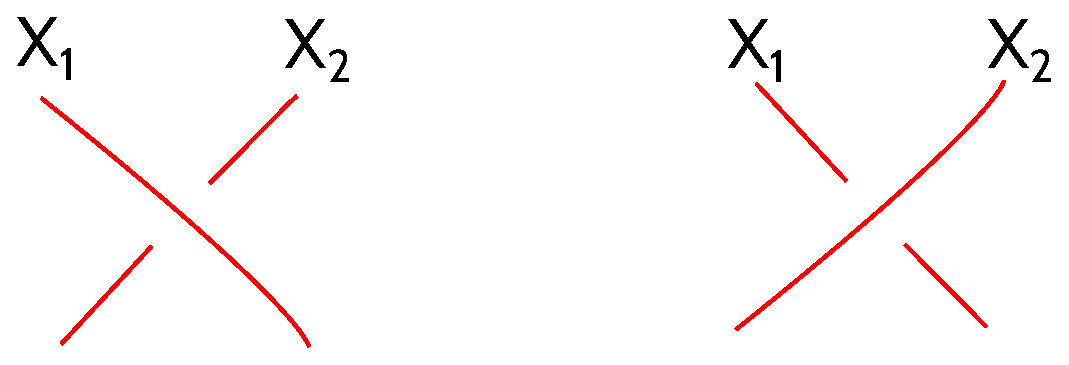
\includegraphics[width=0.4\textwidth]{braiding.eps}
\end{center}
\begin{Def}

A \textit{braided monoidal category} is a monoidal category with a braiding.

\end{Def}
\begin{Def}
A \textit{braided monoidal functor} $F:\C\ra\D$ is a monoidal functor which makes the following diagram commute for any $X, Y \in \C$.
\[
\xymatrix{FX \otimes FY \ar[r]^{\sigma'_{FX, FY}} \ar[d]_{J_{X, Y}} & FY \otimes FX \ar[d]^{J_{Y,X}}\\
F(X\otimes Y) \ar[r]^{F(\sigma_{X, Y})} & F(Y\otimes X)}
\]
\end{Def}

\begin{Expl}\rm
For an abelian group $G$, let $q:G\rightarrow \kk^\times$ be a \textit{quadratic form} (i.e. such that $q(g)= q(g\inv)$ for $g\in G$). For $g, g', h \in G$, the function \begin{equation}
	b(g, h) = \frac{q(gh)}{q(g)q(h)}
\end{equation} is symmetric, \begin{equation}
	b(g, h) = b(h, g),
\end{equation} and is a bicharacter, \begin{equation}
	b(gg', h) = b(g, h) b(g', h).
\end{equation}
We call $q$ \textit{degenerate} if $b$ is degenerate. A quadratic form can be constructed by picking a bicharacter $B$ and setting \begin{equation}
	q(g) = B(g,g).
\end{equation}
\begin{Def}
A \textit{pre-metric group} is a pair $(G, q)$ where $G$ is an abelian group and $q$ is a quadratic form. A \textit{metric group} is a metric group with a non-degenerate quadratic form.	
\end{Def}
\begin{Def}
An \textit{orthogonal homomorphism} between metric groups $(G, q)$ and $(G', q')$ is a group homomorphism $f:G\rightarrow G'$ such that \begin{equation}
	q'\circ f = q.
\end{equation}
\end{Def}
Let $\C$ be a pointed braided fusion category, the simple objects forming a group $G$ following section \ref{pfc}. For a simple object $X\in \OO(\C)$ of degree $g$, define the form $q(g) = \sigma_{X, X} \in \kk$, where $c_{X, X}$ denotes the braiding of $X$ with itself. Assuming that $\C$ is strict, \begin{equation}
	q(gh) = q(g)q(h)b(g,h), g, h\in G
\end{equation}
where $b(g, h)  = c_{Y, X} \circ c_{X, Y}\in \Aut(X\ot Y) \in \kk^\times$ and $g$ and $h$ are the elements associated with the isomorphism classes of $X$ and $Y$ respectively. The fact that $b$ is a bicharacter is a direct consequence of the hexagon axiom (\ref{hex}), and hence $q$ is quadratic form.
One may similarly define a function $\omega: G\times G \times G \ra \kk^\times$ for the associativity morphism, and the pentagon axiom along with the two hexagon axioms yields a set of conditions on the functions $\omega$ and $\sigma$.
\begin{align*}
 	\omega(g_1g_2, g_3, g_4) \omega(g_1, g_2, g_3g_4) = \omega(g_1, g_2, g_3) \omega(g_1, g_2g_3, g_4) \omega(g_2, g_3, g_4)\\
 	\omega (g_2, g_3, g_1) \sigma(g_1, g_2g_3) \omega(g_1, g_2, g_3) = \sigma(g_1, g_3) \omega(g_2, g_1, g_3) \sigma(g_1, g_2)\\
 	\omega(g_3, g_1, g_2)\inv \sigma(g_1g_2, g_3) \omega(g_1, g_2, g_3) \inv = \sigma(g_1, g_3) \omega(g_1, g_3, g_2)\inv \sigma(g_2, g_3),
 \end{align*}for $g_1, g_2, g_3, g_4 \in G$. Couples $(\omega, \sigma)$ satisfying this condition form a group $Z_{ab}^3(G, \kk^\times)$. There is also a parametrization for isomorphism classes of braided functors between pointed braided fusion categories, as the group $B^3(G, \kk^\times)$. Consequently, one can define the so-called \textit{abelian cohomology} of a group $G$ with coefficients in $\kk^\times$, for more details see \cite[Section 8.4]{EGNO}.
\end{Expl}
\begin{Def}
A braided monoidal category $\C$ is \textit{symmetric} if for all objects $X, Y \in \C$, \begin{equation}
	\sigma_{Y, X} \circ \sigma_{X, Y} = \id_{X\otimes Y}. 
\end{equation}

\end{Def}
\subsection{Modularity}
\begin{Def}\rm\label{twistdef}
 A \textit{ribbon structure} on a braided pivotal fusion category is a distinguished isomorphism for every object $X\in \C$,
\begin{align}
\theta_X: X \rightarrow X\nonumber
\end{align}
defined by \begin{equation}
 	 \theta_X = (\ev_X \otimes j_X)\circ(\id_{X^*} \otimes \sigma_{X^{**}, X})\circ(\coev_{X^*} \otimes \id_X),\label{thetax} 
 \end{equation}
 where $\coev_X:\mathbbm{1}\rightarrow X\otimes X^*$ and $\ev_X:X^*\otimes X\rightarrow \mathbbm{1}$ denote the rigidity maps, such that for any objects $X,Y \in \C$, \begin{align}
\theta_{X\otimes Y} &= \sigma_{Y,X}\sigma_{X,Y}(\theta_X\otimes \theta_Y)\label{twist}\\
\theta_{X^*}&=\theta_X^*. \label{twistdual}
\end{align}
 \end{Def}
Graphically, the ribbon structure $\theta_X$ is denoted as follows.

\begin{center}
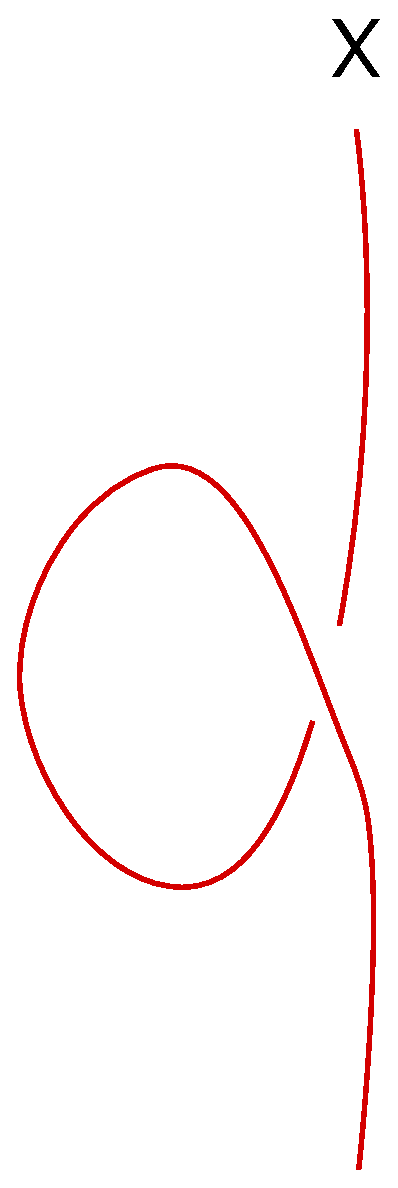
\includegraphics[width=0.1\textwidth]{t-matrix.eps}
\end{center}

 As is clear from formula (\ref{thetax}), the ribbon structure is completely determined by the braiding and pivotal structure, and so every pivotal braided fusion category can be endowed with a ribbon structure in this way. The conditions (\ref{twist}) and (\ref{twistdual}) give the compatibility of the ribbon structure with the braiding and rigid structures respectively. A rigid monoidal category with a ribbon structure is called a \textit{ribbon} category.  The morphism $\theta$ is sometimes called the \textit{twist}.\\
\begin{defn}\label{mfcdef}\rm
A \textit{modular fusion category} $\Cat$ is a ribbon fusion category such that any object $X$ for which \begin{equation}\label{muger}
	\sigma_{Y,X}\sigma_{X,Y}= \id_{X\otimes Y}\end{equation}
 holds for every $Y\in \Cat$, is isomorphic to $\one$.
\end{defn}
The condition on X in the definition above is known as the \textit{non-degeneracy} condition. There are other known definitions of non-degeneracy in the literature but they are all equivalent as shown in \cite{Sh}.\\ 
 


\subsubsection{The Drinfeld center}
The Drinfeld center of a category $\C$, $\CTR(\C)$ is a construction which, starting from a monoidal category, yields a braided monoidal category. Let $\C$ be a monoidal category with associator \begin{equation}
	a_{W, X, Y}: W\otimes (X \otimes Y) \rightarrow (W\otimes X) \otimes Y. 
\end{equation}
An object of $\CTR(\C)$ is the data $(X, \gamma_X)$, where $X\in \C$, and $\gamma$ is a functorial isomorphism \begin{equation}
	\gamma_X: X\otimes - \cong -\otimes X
\end{equation} such that the axioms for a braided category hold. 
 \begin{align} 
\xymatrix { X\ot (Y \ot Z) \ar[r]^{\alpha_{X, Y, Z}}\ar[d]^{\gamma_{Y\ot Z}} & (X\ot Y) \ot Z \ar[r]^{\gamma_Y\ot \id_Z} & (Y\ot X)\ot Z \ar[d]^{\alpha_{Y, X, Z}} \\
(Y\ot Z)\ot X \ar[r]^{\alpha\inv_{Y, Z, X}} & Y\ot (Z \ot X) & Y\ot (X \ot Z)\ar[l]^{Y\ot \gamma_Z}\\}
\end{align}
The morphism $\gamma$ is sometimes called the `half-braiding' (it being functorial in only one variable, as opposed to a braiding which is functorial in both variables).
The space of morphisms $\Hom_{\CTR(\C)}((X, \gamma_X), (X', \gamma_{X'}))$ consists of morphisms $f\in \Hom_\C(X, X')$ that is compatible with the half-braidings on $X$ and $X'$.
\begin{equation}
 	\xymatrix{X\otimes - \ar[r]^{\gamma_X} \ar[d]_{f\otimes \id_-} & - \otimes X \ar[d]^{\id_- \otimes f} \\
 	 	X'\otimes - \ar[r]^{\gamma_{X'}} &-\otimes X' }
 \end{equation}
 The tensor product of two objects, $(X, \gamma_X), (X', \gamma'_{X'})$, is the object $(X\otimes X', \gamma_{X\ot X'})$, $\gamma_{X\ot X'}$ being the half-braiding that makes the following diagram commute. \begin{equation}
 	 \xymatrix{(X\otimes X') \otimes Y \ar[r]^{\alpha_{X, X', Y}} \ar[d]^{\sigma_{X\ot X', Y}} & X\otimes (X' \otimes Y)& X\otimes (Y \otimes X') \ar[l]_{\id_X \ot \sigma_{X', Y}} \\
 	  Y\otimes (X \otimes X') \ar[r]^{\alpha_{Y, X, X'}} &  (Y\otimes X)\otimes X'\ar[r]^{\sigma_{Y, X}} & (X \otimes Y) \otimes X' \ar[u]^{\alpha_{X, Y, X'}}  }
 \end{equation}
 Similarly, if $f:(X, \gamma_X)\rightarrow (X', \gamma_{X'})$ and $f': (Y, \gamma_Y) \rightarrow (Y', \gamma_{Y'})$ are two morphisms in $\CTR(\C)$, then $f\otimes f'$ is also a morphism in $\CTR(\C)$.

If an object $Z\in \C$ has a left dual $Z^*$ then $(Z, \gamma)$ has a left dual $(Z^*, \gamma_{Z^*})$, with $\gamma_{Z^*}$ defined by the composition\begin{equation}
	\gamma_{Z^*}: Z^*\otimes - \xrightarrow{\id_{Z^*\otimes -} \otimes \coev_Z} Z^*\otimes - \otimes Z\otimes Z^* \xrightarrow{\id_{Z^*}\otimes \gamma_Z\inv \otimes \id_Z^*} Z^*\otimes Z \otimes - \otimes Z^*  \xrightarrow{\ev_Z \otimes \id_{-\otimes Z^*}} -\otimes Z^*,
\end{equation} 
a similar definition can be given for a right dual.

There is an obvious forgetful functor $\CTR(\C)\rightarrow \C$, that forgets the half-braiding on each object,
\begin{equation}
	(X, \gamma)\mapsto X.
\end{equation}

\begin{Prop}
There is a canonical equivalence \begin{equation}
	\CTR(\C) \cong (\C\boxtimes \C^{op})^*_{\C} ,
\end{equation} and in particular, the center of a fusion category is also a fusion category.
\end{Prop}
\begin{proof}
A $\C$-bimodule endofunctor $F$ is in particular a left $\C$-module functor, and so $F= -\ot Z$ for some object $Z\in \C$. It is a right $\C$-module functor as well so we have a natural isomorphism \begin{equation}
	(X\ot Y) \ot Z = F(X\ot Y) \xra{s_{X, Y}} F(X) \ot Y = (X\ot Z)\ot Y,
\end{equation}
and the half-braiding associated with $Z$ may be defined as \begin{equation}
	 \gamma = s\inv_{\one, -}: Z \ot - \xra{\sim} -\ot Z.
\end{equation}
Consider the hexagon axiom for the module functor $F$
\[
\xymatrix{
X \ot (Y\ot Z) \ar[r]^{\id_X \ot s\inv_{\one, Y}} & X \ot (Z \ot Y)\ar[r]^{m_{X, Z, Y}} & (X\ot Z) \ot Y \ar[d]^{s\inv_{\one, X} \ot Y} \\
(X\ot Y )\ot Z \ar[u]^{m_{X, Y, Z}}& Z\ot (X\ot Y)\ar[l]_{s\inv_{\one, X\ot Y}} & (Z \ot X) \ot Y. \ar[l]_{m_{Z, X, Y}}  \\   
}
\]
The two arrows on top compose to give the morphism $s_{X, Y}$, which turns the above diagram into a pentagon, and it is easily seen that this is the pentagon axiom for the right $\C$-module category $\C$. Thus the hexagon condition is satisfied for our definition of $\gamma$.
For bimodule endofunctors $F$ and $G$, let $F= -\ot Z$ and $G = -\ot W$ for object $W, Z \in \C$, then the composition \begin{equation}
	GF(X\ot Y) \xra{\sim} G(F(X)\ot Y) \xra{\sim}(GF(X) \ot Y)
\end{equation} yields the braiding associated with the object $Z\ot W$ and so the functor $G\circ F$ is given by the tensor product of the corresponding objects in the center.
\end{proof}

\begin{Prop}\label{centereqv}
The category $(\C\boxtimes \C^*_\M)^*_\M$ is tensor equivalent to $\CTR(\C)$.
\end{Prop}
\begin{proof}
An object of $(\C\boxtimes \C^*_\M)^*_\M$ is a $\C\boxtimes \C^*_\M$-module endofunctor of $\M$, and in particular it is a $\C^*_\M$-module endofunctor, which by Theorem \ref{can} is isomorphic to one of the form $Z\ot -$ for some object $Z\in \C$. We then have an isomorphism for \begin{equation}
	X\ot F(Z\ot -) \cong Z\ot(X\ot F(-)),
\end{equation}for $F\in \C^*_M$ and $X \in \C$, which is the $\C \boxtimes \C^*_\M$ module functor structure. If we let $F=\id$, then we get an isomorphism of $\C^*_\M$-module functors \begin{equation}
	X\ot Z \ot -\xra{\sim} Z\ot X\ot -.
\end{equation}
By the equivalence \ref{can}, $X\mapsto X\ot -$ for $X\in \C$. 

\end{proof}
\begin{Prop}
There is a tensor equivalence \begin{equation}
	\CTR(\C)\cong \CTR(\C^*_\M).
\end{equation}
\begin{proof}
In the statement of Proposition \ref{centereqv}, if we substitute $\C$ by $\C^*_\M$, then we get 
\begin{equation}
	(\C^*_\M \boxtimes (\C^*_\M)^*_\M)^*_\M \cong \CTR(\C^*_\M),
\end{equation} but using Proposition \ref{can} we can write \begin{equation}
	(\C^*_\M \boxtimes \C)^*_\M \cong \CTR(\C^*_\M)
\end{equation} but the left hand side is equivalent to $\CTR(\C)$ so the claim follows.
\end{proof}
\end{Prop}

 The non-degeneracy condition in Definition \ref{mfcdef} is expressed as the non-degeneracy of the symmetric matrix $S$, 
\begin{equation}\label{S}
	S: S_{ij}= \text{tr}(\sigma_{X_j,X_i^*}\circ\sigma_{X_i^*,X_j}),
\end{equation}
where \begin{align}
	\text{tr}(\sigma_{Y,X^*}\circ\sigma_{X^*,Y}) = ((\ev_{X^*}\otimes \ev_{Y^*}) \circ (\j_{X}\inv\circ\id_{X^*} \otimes j_Y\inv \otimes \id_{Y^*}))\circ\\ (\id_X\otimes (\sigma_{Y,X^*}\circ\sigma_{X^*, Y}) \otimes \id_{Y^*})\circ (\coev_X \otimes \coev_Y) \label{Strace}
\end{align}

for $X,Y \in \mathcal{\OO(\Cat)}$, where tr denotes the quantum trace. Graphically this is represented as the closure of a double braiding, as follows.
\begin{center}
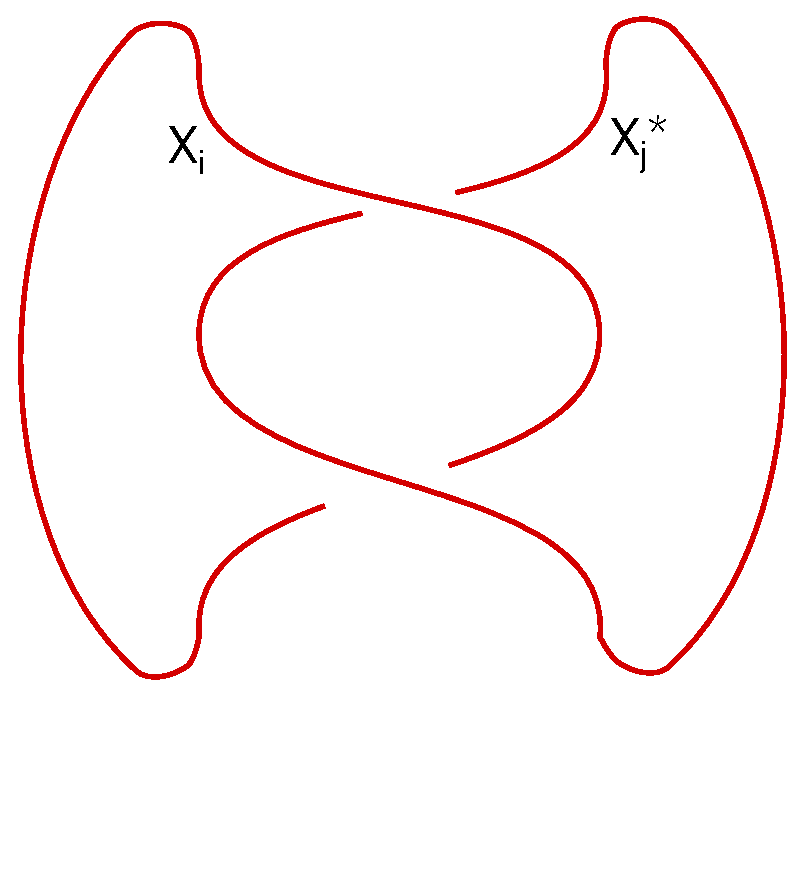
\includegraphics[width=0.2\textwidth]{s-matrix.eps}
\end{center}
For a simple object $X_i$ ($i\in \mathcal{I}$), the morphism $\theta$ (see \ref{twistdef}) is a scalar matrix $\omega_i \id_{X_i}$. The diagonal matrix $T$ is defined as 

\begin{equation}\label{T}
	T: T_{ii} = \omega_i.
\end{equation}
By Vafa's theorem (see\cite{BK}, Theorem 3.1.19), the $T$-matrix has finite order, so the $\omega_i$'s are roots of unity. The order of the $T$-matrix is called the exponent of the MFC, which is also a useful invariant.\\
The data of the $S$-matrix and $T$-matrix is together called the \textit{modular data}. It gives rise to a projective representation of the modular group $\text{SL}_2(\Z)$ which is also the mapping class group of the torus. While the $S$ and $T$ matrices provide a lot of information about the MFC they arise from, they do not serve as complete invariants for MFCs, i.e., two MFCs that are non-equivalent as braided tensor categories may give rise to the same modular data. \cite{2017arXiv170802796M}

\subsection {The Drinfeld center of $\Vect^\omega_G$}\label{CenterVecOmegaG}
We now describe the structure of the Drinfeld center of $\Vect^\omega_G$, $\mathcal{Z}(\Vect^\omega_G)$. The structure of an object $(W,\sigma_{\cdot,W})$ in the center, with $\sigma_{V,W}\colon V\ot W\to W\ot V$ the half-braiding for $V\in\Vect_G^\omega$ can be described in terms of an action (not quite a group action) of $G$ on $W$ \cite{Maj:QDQHA}. More precisely, giving a half-braiding is equivalent to giving a map
$\hit\colon G\otimes W\to W$ subject to the conditions
\begin{align}
  |g\hit w|&=g\hit|w|\\
  e\hit w&=w\\
  g\hit h\hit w&=\alpha_{|w|}(g, h)gh\hit w
\end{align}
for $g,h\in G$ and $w\in W$, and $|\cdot|$ denotes the degree of the element $\cdot$. The braiding isomorphism is described by the formula
\begin{equation*}
  V\ot W\ni v\ot w\mapsto |v|\hit w\ot v\in W\ot V.
\end{equation*}

Let $V\in\CTR(\Vect_G^\omega)$. Since acting by an element $g\in G$ is a vector space automorphism of $V\in\Vect_G^\omega$ which conjugates degrees, any object decomposes as the direct sum of objects where the degrees of nonzero homogeneous components form a conjugacy class. Assume that the degrees of the nonzero components of $V$ form a conjugacy class. Then $G$ permutes those homogeneous components transitively, and elements in the centralizer $C_G(g)$ map the homogeneous component $V_g$ to itself. In particular, $V_g$ is an $\alpha_g$-projective representation of $C_G(g)$ where
\begin{equation}\label{alpha}
\alpha_g(x,y)=\omega(x,y,g)\omega^{-1}(x,y \hit g,y)\omega(xy \hit g ,x ,y)
\end{equation}
and the structure of $V$ is determined by this projective representation for any one $g$ in the conjugacy class. In particular, simple objects of $\CTR(\Vect_G^\omega)$ are parametrized by pairs $(g,\chi)$ where $g$ runs through a system of representatives for the conjugacy classes of $G$, and $\chi$ is an irreducible $\alpha_g$-projective character of $C_G(g)$.

It is convenient to note, for later, how to obtain the $C_G(x)$-projective character $\chi'$ describing the action of $C_G(x)$ on $V_x$ when $x$ belongs to the same conjugacy class, say $x=f\hit g$. So let $c\in C_G(x)$ and $v\in V_g$. We have

\begin{align}\label{1}
c \hit (f \hit v) &= \alpha_{g}(c, f) cf \hit v\\
f \hit ((f\inv\hit c) \hit v)   &= \alpha_{g}(f, f^{-1}\hit c) cf \hit v
\end{align}
and therefore
\begin{equation*}
  c\hit f\hit v  = \alpha_{g}(c, f) \alpha_{g}\inv(f, f^{-1}\hit c) f \hit (f\inv\hit c)\hit v .
\end{equation*}
This means that the diagram
\begin{equation*}
\xymatrix {V_g \ar[rr]^{f\hit} \ar[dd]_{(f^{-1} \hit c)\hit}   & & V_x \ar[dd]^{c\hit}\\
\\
 V_g \ar[rr]^{f\hit}  & & V_x}
\end{equation*}
commutes up to the scalar factor $\alpha_{g}(c, f) \alpha_{g}\inv(f, f^{-1}\hit c)$. By cyclicity of the trace, the projective character of the projective $C_G(x)$-representation $V_x$ is therefore $\chi^x$, given by
\begin{equation}\label{chi}
  \chi^x:=(f\hit\chi)(c):=\alpha_{g}(c, f) \alpha_{g}\inv(f, f^{-1}\hit c)\chi(f\inv\hit c).
\end{equation}
In particular this expression does define a projective character, and does not depend on the choice of $f\in G$ with $f\hit g=x$.

The inverse of the braiding in $\CTR(\Vect_G^\omega)$ is given by $\sigma\inv(w\ot v)=v\ot |v|\inv\bhit w$, where $\bhit\colon\CC G\otimes V\to V$ is such that $g\hit g\inv\bhit v=g\inv\bhit g\hit v=v$. From
\begin{align*}
  f\inv \hit (f \hit v) &= \alpha_{|v|}(f\inv, f) v,\\
  f\hit f\inv\hit v&=\alpha_{|v|}(f,f\inv)v
\end{align*}
one reads off
\begin{align}\label{blackhit}
f\inv\bhit v&=\alpha_{|v|}\inv(f,f\inv) f\inv\hit v,\\
  f\inv\bhit v&=\alpha_{f\hit|v|}\inv(f\inv,f) f\inv\hit v,
\end{align}
respectively.


\iffalse

\subsection{Modular fusion categories of rank 2}
Let $\Cat$ be an MFC of rank 2, $\OO(\Cat) =\{ \mathbbm{1},X\}$. The only non-trivial fusion rule is $X\otimes X \cong \one \oplus nX$, for $n\geq 0$.  By \ref{simpledual}, the object $X$ is self-dual. The unit object $\one$ has fixed multiplicity 1 because of \ref{onemultiplicity}.
It is shown in \cite{O} that $n$ can only be $0$ or $1$ if $\Cat$ is modular. For $n=0$ the fusion ring is isomorphic to $\Z[x]/x^2-1$ and for $n=1$ it is isomorphic to $\Z[x]/x^2 -x -1$.
In this section, although we have only one non-trivial object $X$, we will sometimes use numbering $X_1, X_2 \dots$ when we consider braiding morphisms between tensor powers of $X$. This is only meant to be a convenient way to keep track of objects while braiding. In this section we will denote the associator by $a$ rather than $\alpha$ to avoid confusion later.

\subsubsection{The semion fusion rule $X\otimes X = \one$}\label{semion}

 We only get an mfc if the associativity morphism $(X\otimes X) \otimes X\rightarrow X\otimes (X\otimes X)$ is the negative identity morphism. We calculate the braiding $\sigma_{X,X}: X\otimes X \rightarrow X\otimes X$ using the following braiding hexagon.
 Since $X\otimes X\simeq \mathbbm{1}$, the braiding $\sigma_{X,X}\in \text{End}(\mathbbm{1})$ must be a scalar, \ie \begin{equation}
 	\sigma_{X,X} = \sigma \id_{X\otimes X}, \quad \sigma\in \CC^\times.
 \end{equation} This also means $\sigma_{X_1\otimes X_2, X_3}$ must be trivial (here we have used convention introduced in the beginning of this section). The commutative diagram (\ref{hex2}) gives us
\begin{align}
\sigma_{X_1\otimes X_2, X_3} &=   (a\inv_{X_3,X_1,X_2})\circ (\sigma_{X_1,X_3}\otimes \text{id}_{X_2})\circ(a\inv_{X_1, X_3,X_2}) \circ (\text{id}_{X_1}\otimes \sigma_{X_2, X_3})\circ a_{X_1, X_2, X_3}\nonumber\\
\sigma_{X_1\otimes X_2, X_3} &= - \sigma^2\nonumber\\
\sigma^2 &= -1\nonumber\\
\sigma &= \pm i\nonumber
\end{align} 
For the pivotal structure, which is a monoidal functorial isomorphism $j:**\rightarrow \id$, where $**$ is the double dual functor. We calculate $\theta_X=\theta$, which is also a scalar, using the equation (\ref{twist}), 
 \begin{align}
\theta_{X \otimes X} &= \sigma^2(\theta_X \otimes\theta_X)\nonumber\\
\theta_{1} &= \sigma^2\theta^2\text{id}_{X\otimes X}\nonumber\\
\theta^2 &= \frac{1}{ \sigma^2}\nonumber\\
\theta &= \pm i. \nonumber
 \end{align}

 The T-matrix is then $T= \tmt{1}{0}{0}{\pm i}$.
\\
The rigidity morphisms $\ev: X\otimes X \rightarrow \one$ and $\coev:\one\rightarrow X\otimes X$, must satisfy
\begin{align}
(\text{id}_X\otimes \ev_X) \circ a_{X,X,X}\circ(\coev_X\otimes \text{id}_X) = \text{id}_X. \label{rigid}
\end{align}
However, $a_{X,X,X}=-1$, so we choose $\ev_X = \text{id}_{\mathbbm{1}}$ and $\coev_X=  -\text{id}_{\mathbbm{1}}$ so that \ref {rigid} is satisfied.
Further, since the pivotal structure is a monoidal functorial isomorphism, we have \begin{equation}
	j_\one = j_X^2,\nonumber
\end{equation}and so $j_X=\pm \id_X$ are valid choices for the pivotal structure on $X$.\\ 
We now compute the entries of the $S$-matrix, starting with \begin{equation}
	S_{X, X} = \tr(\sigma_{X, X}^2) =  \tr(\sigma^2 \id_{X\otimes X}),
\end{equation} and using the formula (\ref{Strace}), we get \begin{equation}
	S_{X,X} = -1,
\end{equation} irrespective of the choice of $j_X$.
Similarly, 
\begin{equation}
 	S_{X, \one} = \begin{cases} 1 &  j_X = \id_X, \\ \\-1 & j_X = -\id_X, \end{cases} 
 \end{equation} and $S_{\one, \one} = 1$.
 So depending on the choice of  the pivotal structure $j_X$, we obtain two possible $S$-matrices.
\begin{equation}
	S= \tmt{\ 1}{\ 1 }{\ 1}{-1} \quad \text{or} \quad S=\tmt{\ 1}{-1}{-1}{-1}
\end{equation}

There are thus four sets of modular data for the fusion rule $X\otimes X = \one$.
\begin{center}
\begin{tabular}{ | c  |c | c | c | c  | c | c | c | c | c |c | c |}
\hline
$S$ & $T$ \\ 
\hline
  $\tmt{1}{1}{1}{-1}$ & $\tmt{1}{0}{0}{\pm i}$  \\
 \hline
 $\tmt{1}{-1}{-1}{-1}$ & $\tmt{1}{0}{0}{\pm i}$  \\ 
 \hline
\end{tabular}
\end{center}

\subsubsection{The Fibonacci fusion rule $X\otimes X \cong \one \oplus X$}\label{yanglee}
As before, we first begin by determining the values of the associator $a$ on triples of simple objects.
The only non-trivial associator is $a_{X, X, X}:(X\otimes X) \otimes X\rightarrow X\otimes (X\otimes X)$, but this time the task is more complicated than the previous case. To treat it, we introduce some general theory for computing associators in a special case, following \cite{TY}. The following techniques are classical in conformal field theory literature, although terminology differs. 

Let $\mathcal{C}$ be a fusion category, whose fusion rules do not have multiplicites greater than 1, i.e., dim $\text{Hom}(M, N\otimes Q) \leq 1$ for $M, N, Q \in \mathcal{\OO(\Cat)}$. Such a fusion ring is called a \textit{hyperring} in \cite{davidovich2013arithmetic}.    Suppose $N$ has multiplicity 1 in $N\otimes Q$. Let a basis element of the one-dimensional vector space $\text{Hom}(M, N\otimes Q)$ be denoted by
\begin{center}
	\begin{tikzpicture}[grow'=up]
            \Tree [.M [.N ] [ .Q  ] ]
	\end{tikzpicture}.
\end{center}
For simple objects $A, B, C \in \OO(\Cat)$, the existence of the associativity morphism $a_{A, B, C}: A\otimes (B \otimes C)\rightarrow (A\otimes B)\otimes C $ leads to an isomorphism
\begin{equation}
	\text{Hom} (D, a_{A,B,C}):  \text{Hom}(D, (A\otimes B) \otimes C)\rightarrow\text{Hom}(D, A\otimes (B\otimes C)),\label{alpha}
\end{equation}
for every  $D\in \OO(\Cat)$.
Further, there are isomorphisms 
\begin{equation}
\begin{array}{cccc}

	 \text{Hom}(D, (A\otimes B) \otimes C) \simeq \underset{F\in \OO(\Cat)}\bigoplus \C& \Bigg(\vcenter{\hbox{\begin{tikzpicture}[grow'=up]\Tree [.D [.F [.A ] [.B ] ] [ C  ] ]\end{tikzpicture}}}\Bigg)

\end{array}
\end{equation}
\begin{equation}
\begin{array}{cccc}

	 \text{Hom}(D, A\otimes (B \otimes C)) \simeq \underset{F\in \OO(\Cat)}\bigoplus \C & \Bigg(\vcenter{\hbox{\begin{tikzpicture}[grow'=up]\Tree [.D [ A  ] [.F [.B ] [.C ] ]  ]\end{tikzpicture}}}\Bigg) , 

\end{array}
\end{equation} where the right hand sides are direct sums of the $\CC$-spans of a choice of basis vectors for
 the spaces $\text{Hom}(D, F\otimes C) \otimes \text{Hom}(F, A\otimes B)$ and $\text{Hom}(D, A\otimes F) \otimes \text{Hom}(F, B\otimes C)$ respectively. 
Now (\ref{alpha}) can be written as
\begin{equation}
\begin{array}{ccccccc}

	 	\text{Hom} (D, a_{A,B,C}): \underset{F\in \OO(\Cat)}\bigoplus \C & \Bigg(\vcenter{\hbox{\begin{tikzpicture}[grow'=up] \Tree [.D [.F [.A ] [.B ] ] [ C  ] ]\end{tikzpicture}}}\Bigg)  \rightarrow \underset{F\in \OO(\Cat)}\bigoplus \C& \Bigg(\vcenter{\hbox{\begin{tikzpicture}[grow'=up] \Tree [.D [ A  ] [.F [.B ] [.C ] ]  ]\end{tikzpicture}}}\Bigg)

\end{array}
\end{equation}
 and now we can determine $\Hom(D, a_{A, B, C})$ for every $D\in \OO(\Cat)$, which is as good as determining the morphism $a_{A,B,C}$. 
Now, let $\Cat$ be a fusion category with  $\OO(\Cat)=\{\one, X\}$ and fusion rule $X\otimes X \cong \one\oplus X$. In the above calculation, let $A=B=C=X$, then for $D=X$, 

\begin{equation}
\begin{array}{ccccccc}\C\Bigg(
\vcenter{\hbox{\begin{tikzpicture}[grow'=up]
            \Tree [.X [.$\one$ [.X ] [.X ] ] [ X  ] ]
\end{tikzpicture}}}\Bigg)
& \oplus 
&
\C\Bigg(\vcenter{\hbox{\begin{tikzpicture}[grow'=up]
            \Tree [.X [.X [.X ] [.X ] ] [ X  ] ]
\end{tikzpicture}}}\Bigg)
&
\rightarrow
&
\C\Bigg(\vcenter{\hbox{\begin{tikzpicture}[grow'=up]
 \Tree [.X [ X  ] [.$\one$ [.X ] [.X ] ]  ]
\end{tikzpicture}}}\Bigg)
&
\oplus
&
\C\Bigg(\vcenter{\hbox{\begin{tikzpicture}[grow'=up]
 \Tree [.X [ X  ] [.X [.X ] [.X ] ]  ]
\end{tikzpicture}}}\Bigg)
\end{array}
\end{equation}
In this basis, the map $\text{Hom}(X, a_{X,X,X})$ should be given by  $\tmt{\alpha}{\beta}{\gamma}{\delta} \in \text{GL}_2(\CC)$. Let the basis elements be mapped in the following way. 
\begin{equation}\label{a1}
\begin{array}{ccccccc}
\vcenter{\hbox{\begin{tikzpicture}[grow'=up]
            \Tree [.X [.$\one$ [.X ] [.X ] ] [ X  ] ]
\end{tikzpicture}}}
&
\xmapsto{a_{X,X,X}}
&
\alpha
&
\vcenter{\hbox{\begin{tikzpicture}[grow'=up]
 \Tree [.X [ X  ] [.$\one$ [ .X ] [.X ] ]  ]
\end{tikzpicture}}}
&
+
&
\beta
&
\vcenter{\hbox{\begin{tikzpicture}[grow'=up]
 \Tree [.X [ X  ] [.X [ .X ] [.X ] ]  ]
\end{tikzpicture}}}
\end{array}
\end{equation}
\begin{equation}\label{a2}
\begin{array}{ccccccc}
\vcenter{\hbox{\begin{tikzpicture}[grow'=up]
            \Tree [.X [.X [.X ] [.X ] ] [ X  ] ]
\end{tikzpicture}}}
&
\xmapsto{a_{X, X, X}}
&
\gamma
&
\vcenter{\hbox{\begin{tikzpicture}[grow'=up]
 \Tree [.X [ X  ] [. $\one$ [.X ] [.X ] ]  ]
\end{tikzpicture}}}
&
+
&
\delta
&
\vcenter{\hbox{\begin{tikzpicture}[grow'=up]
 \Tree [.X [ X ] [.X [.X ] [.X ] ]  ]
\end{tikzpicture}}}
\end{array}
\end{equation}
Note that the arrows labelled $a_{X, X, X}$ actually refer to  $\Hom(X, a_{X, X, X})$. We hope that will it be clear from the basis elements which space is actually meant. Such abuse of notation shall be rampant in the sequel. 
Similarly for $\Hom(\one, a_{X, X, X})$, the elements \begin{equation}
\begin{array}{ccccccc}
\vcenter{\hbox{\begin{tikzpicture}[grow'=up]
            \Tree [.$\one$ [.$\one$ [.X ] [.X ] ] [ X  ] ]
\end{tikzpicture}}},
&
\vcenter{\hbox{\begin{tikzpicture}[grow'=up]
 \Tree [.$\one$ [ X ] [.$\one$ [.X ] [.X ] ]  ]
\end{tikzpicture}}}
\end{array}
\end{equation} are zero since $\Hom(\one, \one \otimes X) = 0$, so $\Hom(\one, a_{X, X, X})$ is a scalar map, \begin{equation}
	\begin{array}{ccccccc}
	\C\Bigg(
\vcenter{\hbox{\begin{tikzpicture}[grow'=up]
            \Tree [.$\one$ [.X [.X ] [.X ] ] [ X  ] ]
\end{tikzpicture}}}\Bigg)
&
\rightarrow
&
\C \Bigg(
\vcenter{\hbox{\begin{tikzpicture}[grow'=up]
 \Tree [.$\one$ [ X ] [.X [.X ] [.X ] ]  ]
\end{tikzpicture}}}\Bigg)
\end{array}
\end{equation} which is given by some $\lambda\in \CC^\times$.
The equations (\ref{assoc1}), (\ref{t1}) represent the clockwise branch and equations (\ref{assoc2}), (\ref{t2}) represent the anticlockwise branch of the pentagon identity.
\begin{equation}\label{assoc1}
\begin{array}{ccccccc}
\vcenter{\hbox{\begin{tikzpicture}[grow'=up]
            \Tree [.X [.X [.X [.X ][.X ] ] [ X ] ] [[X ]  ] ]
\end{tikzpicture}}}
& 
\xmapsto{a_{X, X, X}\otimes \id_X}
\gamma
&
\vcenter{\hbox{\begin{tikzpicture}[grow'=up]
        \Tree [.X [.X [X ] [ .$\one$  X [.X ]  ]  ] [[X ]  ]  ] 
\end{tikzpicture}}}
&
+ 
&
\delta
&
\vcenter{\hbox{\begin{tikzpicture}[grow'=up]
            \Tree [.X [.X [X ] [ .X  X [.X ]  ]  ] [[X ]]   ] 

\end{tikzpicture}}}
\end{array}
\end{equation}
\[
\begin{array}{ccccccccccc}
\xmapsto{a_{X, X\otimes X, X}}
&
\gamma

\vcenter{\hbox{\begin{tikzpicture}[grow'=up]
        \Tree [.X  [[X ]  ] [.X  [ .$\one$  X [.X ]] [X ]  ]  ] ] 
\end{tikzpicture}}}
&
+ 
&
\delta\gamma
&
\vcenter{\hbox{\begin{tikzpicture}[grow'=up]
            
\Tree [.X  [[X ]  ] [.$\one$ [ .X X [.X ]] [  X   ]  ] ]
\end{tikzpicture}}}  
+ 
&
\delta^2
&
\vcenter{\hbox{\begin{tikzpicture}[grow'=up]
            
\Tree [.X  [[X ]  ] [.X [ .X X [.X ]] [  X   ]  ] ]
\end{tikzpicture}}}  
\end{array}
\]
\[
\begin{array}{ccccccccccc}
\xmapsto{\id_X \otimes a_{X, X, X}} 
\gamma\alpha

\vcenter{\hbox{\begin{tikzpicture}[grow'=up]
        \Tree [.X  [[X ]  ] [.X  [X ]  [ .$\one$  X [.X ]] ]  ] ] 
\end{tikzpicture}}}

+ 
&
\gamma\beta

\vcenter{\hbox{\begin{tikzpicture}[grow'=up]
        \Tree [.X  [[X ]  ] [.X  [X ]  [ .X X [.X ]] ]  ] ] 
\end{tikzpicture}}}

+
&
\delta\gamma\lambda
\vcenter{\hbox{\begin{tikzpicture}[grow'=up]
            
\Tree [.X  [[X ]  ] [.$\one$ [  X ] [ .X X .X  ]  ] ]
\end{tikzpicture}}}  
+ \\

\delta^2\gamma

\vcenter{\hbox{\begin{tikzpicture}[grow'=up]
            
\Tree [.X  [[X ]  ] [.X [  X ] [.$\one$   X   [.X ]]  ] ]
\end{tikzpicture}}}  
+ 
\delta^3

\vcenter{\hbox{\begin{tikzpicture}[grow'=up]
            
\Tree [.X  [[X ]  ] [.X [  X ] [.X  X   [.X ]]  ] ]
\end{tikzpicture}}}  
\end{array}
\]

\begin{equation}\label{assoc2}
\begin{array}{ccccccc}
\vcenter{\hbox{\begin{tikzpicture}[grow'=up]
            \Tree [.X [.X [.X [.X ][.X ] ] [ X ] ] [[X ]  ] ]
\end{tikzpicture}}}
& 
\xmapsto{a_{X\otimes X, X, X}}
&
\gamma

\vcenter{\hbox{\begin{tikzpicture}[grow'=up]
        \Tree [.X [[.X [.X ] [.X ]  ]]  [[ .$\one$   [.X ] [.X ] ] ]   ] 
\end{tikzpicture}}}
&
+ 
&
\delta
&
\vcenter{\hbox{\begin{tikzpicture}[grow'=up]
                   \Tree [.X [[.X [.X ] [.X ]  ]]  [[ .X   [.X ] [.X ] ] ]   ] 

\end{tikzpicture}}}
\end{array}
\end{equation}
\begin{equation*}
\begin{array}{ccccccc}

\xmapsto{a_{X, X, X\otimes X}}
\gamma
\vcenter{\hbox{\begin{tikzpicture}[grow'=up]
        \Tree [.X [[ [.X ]  ]]  [.X [[.X ]][ .$\one$   [.X ] [.X ] ] ]   ] 
\end{tikzpicture}}}
&
+ 
&
\delta\gamma
&
\vcenter{\hbox{\begin{tikzpicture}[grow'=up]
                   \Tree [.X [[ [.X ]  ]]  [.$\one$ [[.X ]][ .X [.X ] [.X ] ] ]   ] 
\end{tikzpicture}}}
&
+
&
\delta^2
&
\vcenter{\hbox{\begin{tikzpicture}[grow'=up]
                   \Tree [.X [[ [.X ]  ]]  [.X [[.X ]][ .X [.X ] [.X ] ] ]   ] 
\end{tikzpicture}}}

\end{array}
\end{equation*}



\begin{equation}\label{t1}
\begin{array}{ccccccc}
\vcenter{\hbox{\begin{tikzpicture}[grow'=up]
            \Tree [.$\one$ [.X [.X [.X ][.X ] ] [ X ] ] [[X ]  ] ]
\end{tikzpicture}}}

&
\xmapsto{a_{X, X, X} \otimes \id_X} 
&
\gamma
\vcenter{\hbox{\begin{tikzpicture}[grow'=up]
        \Tree [.$\one$ [.X [X ] [ .$\one$  X [.X ]  ]  ] [[X ]  ]  ] 
\end{tikzpicture}}}
&
+ 
&
\delta
\vcenter{\hbox{\begin{tikzpicture}[grow'=up]
        \Tree [.$\one$ [.X [X ] [ .X  X [.X ]  ]  ] [[X ]  ]  ] 
\end{tikzpicture}}}

\end{array}
\end{equation}

\[
\begin{array}{ccccccccccc}
\xmapsto{a_{X, X\otimes X, X}}
\gamma

\vcenter{\hbox{\begin{tikzpicture}[grow'=up]
      \Tree [.$\one$  [[X ]  ] [.X [ .$\one$ X [.X ]] [  X   ]  ] ] 
\end{tikzpicture}}}
&
+ 
&
\lambda\delta
&
\vcenter{\hbox{\begin{tikzpicture}[grow'=up]
            
\Tree [.$\one$  [[X ]  ] [.X [ .X X [.X ]] [  X   ]  ] ]
\end{tikzpicture}}}  
\end{array}
\]
\[
\begin{array}{ccccccccccc}
\xmapsto{\id_X\otimes a_{X, X, X}}
\gamma\alpha
&
\vcenter{\hbox{\begin{tikzpicture}[grow'=up]
      \Tree [.$\one$  [[X ]  ] [.X  [  X   ][ .$\one$ X [.X ]]  ] ] 
\end{tikzpicture}}}
&
+ 
&
\gamma\beta 
&
\vcenter{\hbox{\begin{tikzpicture}[grow'=up]
            
\Tree [.$\one$  [[X ]  ] [.X [  X   ] [ .X X [.X ]]  ] ]
\end{tikzpicture}}}
&
+
&
\gamma\lambda\delta
&
\vcenter{\hbox{\begin{tikzpicture}[grow'=up]
      \Tree [.$\one$  [[X ]  ] [.X  [  X   ][ .$\one$ X [.X ]]  ] ] 
\end{tikzpicture}}}
&
+
\delta\lambda\delta
&
\vcenter{\hbox{\begin{tikzpicture}[grow'=up]
            
\Tree [.$\one$  [[X ]  ] [.X [  X   ] [ .X X [.X ]]  ] ]
\end{tikzpicture}}}
\end{array}
\]

\begin{equation}\label{t2}
\begin{array}{ccccccc}
\vcenter{\hbox{\begin{tikzpicture}[grow'=up]
            \Tree [.$\one$ [.X [.X [.X ][.X ] ] [ X ] ] [[X ]  ] ]
\end{tikzpicture}}}

&
\xmapsto{a_{X\otimes X, X, X}} 
&
\lambda
\vcenter{\hbox{\begin{tikzpicture}[grow'=up]
       \Tree [.$\one$ [[.X [.X ] [.X ]  ]]  [[ .X   [.X ] [.X ] ] ]   ] 
\end{tikzpicture}}}
&
\xmapsto{a_{X, X, X\otimes X}}
&
\lambda^2
\vcenter{\hbox{\begin{tikzpicture}[grow'=up]
        \Tree [.$\one$  [[X ]  ] [.X [  X   ] [ .X X [.X ]]  ] ] 
\end{tikzpicture}}}

\end{array}
\end{equation}
Equations (\ref{assoc1}), (\ref{assoc2}), (\ref{t1}) and (\ref{t2}) yield the following conditions,
\begin{align}
\gamma\alpha + \delta^2\gamma &= \gamma \label{1}\\
\gamma\beta+\delta^3 &= \delta^2 \label{2}\\
\lambda\gamma\delta &= \delta\gamma \label{lambda}\\
\lambda\delta^2 + \gamma\beta&=\lambda^2 \label{3}\\
\gamma\alpha + \gamma\lambda\delta &= 0\label{4}.
\end{align}
Equation \ref{lambda} directly tells us that $$\lambda = 1.$$ Assuming $\gamma \neq 0$, From equation\ref{4} we get $$\alpha = -\delta.$$
Substituting in equation \ref{1}, we get \begin{equation}\label{delta}
	\delta^2 = \delta + 1.
\end{equation}
This gives \begin{equation}
	\delta = \bar{\varphi},\text{ where }\bar{\varphi}= \frac{1-\sqrt{5}}2,\label{golden}
\end{equation} a root of the equation $x^2 =x + 1$. Note that we have made a choice here; an equally valid choice would be the other root of this quadratic equation, $\delta =\varphi =  -\frac{1}{\bar{\varphi}} = \frac{1+\sqrt{5}}2$.
Using (\ref{3}), we get$$\gamma\beta = 1-\delta^2$$ and using (\ref{delta}), we get $$\gamma\beta = -\bar{\varphi}.$$ We conclude that $\beta$ and $\gamma$ are free parameters subject to the above condition. We choose $\beta= 1$ and $\gamma = -\bar{\varphi}$,  and we finally get \begin{equation}\label{ass}
	\tmt{\alpha}{\beta}{\gamma}{\delta} = \tmt{-\bar{\varphi}}{1}{-\bar{\varphi}}{\bar{\varphi}}.
\end{equation} 

In the literature, such matrices are called $F$-matrices. Once we have computed this associator, we need to know the possible braidings compatible with it. Let us first explain how we can interpret the braiding morphism in terms of the tree diagrams introduced above. For $A, B, C \in \OO(\Cat)$, let $A$ be a direct summand in $B\otimes C$ and consider the braiding, \begin{equation}
	\sigma_{B,C}: B\otimes C \rightarrow C\otimes B.
\end{equation} This induces an isomorphism of Hom spaces, $\sigma_{B,C}^A:\Hom(A, B\otimes C) \rightarrow \Hom(A, C\otimes B)$, with
\begin{equation}
\begin{array}{ccccccc}
\vcenter{\hbox{\begin{tikzpicture}[grow'=up]
            \Tree [.A   C B  ] 
\end{tikzpicture}}}
\end{array}
:=
\sigma_{B,C}^A  \left(
\begin{array}{ccccccc}
\vcenter{\hbox{\begin{tikzpicture}[grow'=up]
            \Tree [.A   B  C  ] 
\end{tikzpicture}}}
\end{array}
\right).
\end{equation}
 Any morphism maps a copy of $A$ to another one in the target object. Since multiplicities our fusion rules are not greater than 1, $\sigma_{B,C}^A$ is a scalar, and hence the braiding matrix is an $n\times n$ diagonal matrix where $n=|\OO(\Cat)|$. In the case at hand, the only non-trivial braiding is $\sigma_{X,X}: X\otimes X \rightarrow X\otimes X$. As $X\otimes X \simeq \one \oplus X$, $\sigma$ is a diagonal matrix with scalars $c$ and $d$ on the diagonal indicating the scaling for $\one$ and $X$ respectively under the braiding morphism.
\begin{equation}
	\sigma_{X,X}= \tmt{c}{0}{0}{d} \in  \text{GL}_2(\CC).
	\end{equation}
In the following computation, we use the braiding hexagon \ref{hex} to compute values of $c$ and $d$.  We  use \ref{a1} and $\ref{a2}$ where necessary.
\begin{equation}\label{br1}
\begin{array}{ccccccc}
\vcenter{\hbox{\begin{tikzpicture}[grow'=up]
            \Tree [.X [.X [.$\text{X}_1$ ] [.$\text{X}_2$ ] ] [ $\text{X}_3$  ] ]
\end{tikzpicture}}}
&
\xmapsto{}
&
-\bar{\varphi}
&
\vcenter{\hbox{\begin{tikzpicture}[grow'=up]
 \Tree [.X [ $\text{X}_1$ ] [. $\one$ [.$\text{X}_2$ ] [.$\text{X}_3$ ] ]  ]
\end{tikzpicture}}}
&
+
&
\bar{\varphi}
&
\vcenter{\hbox{\begin{tikzpicture}[grow'=up]
 \Tree [.X [ $\text{X}_1$ ] [.X [.$\text{X}_2$ ] [.$\text{X}_3$ ] ]  ]
\end{tikzpicture}}}
\end{array}
\end{equation}

\begin{equation*}
\begin{array}{ccccccc}

\xmapsto{}
&
-\bar{\varphi}
&
\vcenter{\hbox{\begin{tikzpicture}[grow'=up]
 \Tree [.X  [. $\one$ [.$\text{X}_2$ ] [.$\text{X}_3$ ] ] [ $\text{X}_1$  ] ]
\end{tikzpicture}}}
&
+
&
d \bar{\varphi}
&
\vcenter{\hbox{\begin{tikzpicture}[grow'=up]
 \Tree [.X  [.X [.$\text{X}_2$ ] [.$\text{X}_3$ ] ] [ $\text{X}_1$ ] ]
\end{tikzpicture}}}
\end{array}
\end{equation*}
\begin{equation*}
\begin{array}{ccccccc}
\xmapsto{}
&
\bar{\varphi}^2

\vcenter{\hbox{\begin{tikzpicture}[grow'=up]
            \Tree [.X [ $\text{X}_2$  ] [.$\one$ [.$\text{X}_3$ ] [.$\text{X}_1$ ] ]  ]
\end{tikzpicture}}}
&
-\bar{\varphi}
\vcenter{\hbox{\begin{tikzpicture}[grow'=up]
            \Tree [.X [ $\text{X}_2$  ][.X [.$\text{X}_3$ ] [.$\text{X}_1$ ] ]  ]
\end{tikzpicture}}}
&
 -\bar{\varphi}^2 d 

\vcenter{\hbox{\begin{tikzpicture}[grow'=up]
            \Tree [.X [ $\text{X}_2$  ] [.$\one$ [.$\text{X}_3$ ] [.$\text{X}_1$ ] ]  ]
\end{tikzpicture}}}
+ \bar{\varphi}^2 d
\vcenter{\hbox{\begin{tikzpicture}[grow'=up]
            \Tree [.X [ $\text{X}_2$  ][.X [.$\text{X}_3$ ] [.$\text{X}_1$ ] ]  ]
\end{tikzpicture}}}
\end{array}
\end{equation*}

\begin{equation}\label{br2}
\begin{array}{ccccccc}
\vcenter{\hbox{\begin{tikzpicture}[grow'=up]
            \Tree [.X [.X [.$\text{X}_1$ ] [.$\text{X}_2$ ] ] [ $\text{X}_3$  ] ]
\end{tikzpicture}}}
&
\xmapsto{\sigma_{X_1, X_2}\otimes \id_{X_3}}
&
d
\vcenter{\hbox{\begin{tikzpicture}[grow'=up]
            \Tree [.X [.X [.$\text{X}_2$ ] [.$\text{X}_1$ ] ] [ $\text{X}_3$  ] ]
\end{tikzpicture}}}
\end{array}
\begin{array}{ccccccc}
\xmapsto{a_{X_2, X_1, X_3}}
&
-\bar{\varphi} d 

\vcenter{\hbox{\begin{tikzpicture}[grow'=up]
            \Tree [.X [ $\text{X}_2$  ][.$\one$ [.$\text{X}_1$ ] [.$\text{X}_3$ ] ]  ]
\end{tikzpicture}}}
&
+ \bar{\varphi} d
\vcenter{\hbox{\begin{tikzpicture}[grow'=up]
            \Tree [.X [ $\text{X}_2$  ][.X [.$\text{X}_1$ ] [.$\text{X}_3$ ] ]  ]
\end{tikzpicture}}}
\end{array}
\end{equation}

\begin{equation*}
	\begin{array}{ccccccc}
\xmapsto{\id_{X_2}\otimes \sigma_{X_1, X_3}}
&
-\bar{\varphi} c d 

\vcenter{\hbox{\begin{tikzpicture}[grow'=up]
            \Tree [.X [ $\text{X}_2$  ][.$\one$ [.$\text{X}_3$ ] [.$\text{X}_1$ ] ]  ]
\end{tikzpicture}}}
&
+ \bar{\varphi} d^2
\vcenter{\hbox{\begin{tikzpicture}[grow'=up]
            \Tree [.X [ $\text{X}_2$  ][.X [.$\text{X}_3$ ] [.$\text{X}_1$ ] ]  ]
\end{tikzpicture}}}
\end{array}
\end{equation*}

From equations (\ref{br1}) and (\ref{br2}) we have 
\begin{align}
	-\bar{\varphi} + \bar{\varphi} d  &= cd\label{c}\\
	-1 + d\bar{\varphi} &= d^2 \label{d}
\end{align} 
By Vieta's theorem, the solutions of the second equation are multiplicative inverses, let's denote them by $d$ and $d\inv$. Further, \begin{equation}
	d + d\inv = \bar{\varphi}, \label{dsum}
\end{equation} and the equation (\ref{c}) gives\begin{equation}
	c = -\bar{\varphi}\frac{1-d}d = -(d+ d\inv)(\frac{1-d}d) = \bar{\varphi} -1 -\frac{1}{d^2}
\end{equation}
Now if we consider  \begin{equation}
	d^2-c = d^2-\bar{\varphi} + 1 + \frac{1}{d^2} = -\bar{\varphi} -1 + (d+1/d)^2 = - \bar{\varphi} -1 + \bar{\varphi}^2 = 0
\end{equation}
this gives \begin{equation}\label{cdsq}
	c = d^2.
\end{equation}
Since equation (\ref{dsum}) holds,
 \begin{equation}
	(d+d\inv)^2 = (d+d\inv) + 1
\end{equation}
and multiplying throughout by $d^2$ we get \begin{equation}
	1 - d + d^2 - d^3 + d^4 = 0,
\end{equation}
which means $-d$, as well as $-d\inv$, are primitive fifth roots of unity.

Let us determine the possible pivotal structures on modular categories with this fusion rule. Recall that a pivotal structure on a fusion category is a monoidal functorial isomorphism $j: **\rightarrow\text{id}$, where $**$ is the double dual functor. To compute $j$, one must first choose a rigid structure, $\ev_X:X^*\otimes X\rightarrow \one$, and $\coev_X:\one\rightarrow X\otimes X^*$, for each nontrivial object $X$, such that $\ev$ and $\coev$ obey the rigidity axioms. Since in our category $X$ is self dual and $X\otimes X \cong \one \oplus X$, we can choose $\ev= \iota$ and $\coev=\kappa\pi$, for some scalar $\kappa$ where $\iota:\one\rightarrow\one\oplus X$ is the canonical injection and  $\pi: \one\oplus X\rightarrow \one$ is the canonical projection.
For the rigidity conditions (\ref{rigid1}) (\ref{rigid2}), we need
\begin{equation}
	(\id_X \otimes \pi) \circ a_{X, X, X}\circ(\iota \otimes \id_X) = \id_X,
\end{equation}
from which we obtain $\kappa=1/(-\bar{\varphi}) = \varphi$.
Now, the pivotal structure $j$ is such that $j_\one =\id_\one$, and as a consequence of Lemma (\ref{jlemma}), $j_X = \id_X$. 
Hence we have, \begin{align}
	S_{\one,\one} &= \text{tr}(\sigma^2_{\one, \one})=1\\
	S_{\one, X} &= \text{tr}(\sigma_{X, \one} \circ \sigma_{\one, X} ) = \varphi\\
	S_{X, \one} &= \text{tr}(\sigma_{ \one, X} \circ \sigma_{X, \one} )=\varphi\\
	S_{X, X} &= \text{tr}(\sigma^2_{X,X}) =  (d^4 + \varphi d^2) = (d\bar{\varphi} -1)(d\bar{\varphi} -1 + \varphi) = d^2(\bar{\varphi} +1) -2d\bar{\varphi} -d +1 -\varphi\\&= (d\bar{\varphi} -1)(\bar{\varphi} +1) -2d\bar{\varphi} -d +1 -\varphi = d(\bar{\varphi}+1) + d\bar{\varphi} -2d\bar{\varphi} - d -1 = -1,
\end{align}
where we have used (\ref{d}) and the fact that $\bar{\varphi} + \varphi = 1$, $\bar{\varphi}\varphi =-1$.
Thus the $S$-matrix becomes \begin{equation}
	S = \tmt{1}{\varphi}{\varphi}{-1}
\end{equation}
for the choice $\bar{\varphi}$ in the associator matrix (\ref{ass}).

The twist on $\one$, must satisfy \begin{equation}
	\theta_{\one} =\theta_{\one \otimes \one} = \theta_\one^2
\end{equation} 
which means the scalar $\theta_\one =1$. To calculate the twist on $X$, recall that the twist morphism for a simple object X is composition \begin{equation}
	\theta_X =(\ev_{X} \otimes j_X\inv)\circ(\id_{X^*} \otimes \sigma_{X^{**}, X} )\circ(\coev_{X^*} \otimes \id_X):X\rightarrow X.
\end{equation}

If we consider \begin{equation}
	\Hom(X, \theta_X): \Hom (X, X)\rightarrow \Hom(X,X),
\end{equation} this also gives the scalar $\theta$.
In terms of bases, the above equation reads as follows,
\begin{equation}
\begin{array}{ccccccc}
\vcenter{\hbox{\begin{tikzpicture}[grow'=up]
            \Tree [.X [.$\one$ ] [ .X  ] ]
\end{tikzpicture}}}
&
\xmapsto{coev_{X^*} \otimes \id_X} 
\frac{-1}{\bar{\varphi}}
\vcenter{\hbox{\begin{tikzpicture}[grow'=up]
            \Tree [.X [.$\one$ [.$\text{X}^*$ ] [.$\text{X}^{**}$ ] ] [ $\text{X}$  ] ]
\end{tikzpicture}}}
&
\xmapsto{a_{X^*,X^{**}, X}}
&

&
\vcenter{\hbox{\begin{tikzpicture}[grow'=up]
 \Tree [.X [ $\text{X}^*$ ] [. $\one$ [.$\text{X}^{**}$ ] [.$\text{X}$ ] ]  ]
\end{tikzpicture}}}

&
-
&
\frac{1}{\bar{\varphi}}
\vcenter{\hbox{\begin{tikzpicture}[grow'=up]
 \Tree [.X [ $\text{X}^*$ ] [.X [.$\text{X}^{**}$ ] [.$\text{X}$ ] ]  ]
\end{tikzpicture}}}
\end{array}
\end{equation}

\begin{equation*}
	\begin{array}{ccccccc}
\xmapsto{\id_{X^*} \otimes \sigma_{X^{**}, X}}
&
c
\vcenter{\hbox{\begin{tikzpicture}[grow'=up]
            \Tree [.X [ $\text{X}^*$  ][.$\one$ [.$\text{X}$ ] [.$\text{X}^{**}$ ] ]  ]
\end{tikzpicture}}}
&
-\frac{d}{\bar{\varphi}}
\vcenter{\hbox{\begin{tikzpicture}[grow'=up]
            \Tree [.X [ $\text{X}^*$  ][.X [.$\text{X}$ ] [.$\text{X}^{**}$ ] ]  ]
\end{tikzpicture}}}
\end{array}
\end{equation*}
\begin{equation*}
	\begin{array}{cccccc}
\xmapsto{a_{X^*, X, X^{**}}}
&
(-c\bar{\varphi}+d
)&
\vcenter{\hbox{\begin{tikzpicture}[grow'=up]
 \Tree [.X  [. $\one$ [.$\text{X}^*$ ] [.$\text{X}$ ] ] [ $\text{X}^{**}$  ] ]
\end{tikzpicture}}}
&
+
&
(c-d)
&
\vcenter{\hbox{\begin{tikzpicture}[grow'=up]
 \Tree [.X  [.X [.$\text{X}^*$ ] [.$\text{X}$ ] ] [ $\text{X}^{**}$ ] ]
\end{tikzpicture}}}
	\end{array}
\end{equation*}
The map $\ev:X^*\otimes X \rightarrow \one$ is defined to be the canonical projection to $\one$, so we can simply forget the second summand above, and write 
\begin{equation}
	\begin{array}{cccccc}

(-c\bar{\varphi}+d)
&
\vcenter{\hbox{\begin{tikzpicture}[grow'=up]
 \Tree [.X  [. $\one$ [.$\text{X}^*$ ] [.$\text{X}$ ] ] [ $\text{X}^{**}$  ] ]
\end{tikzpicture}}}
&

\xmapsto{\ev_X\otimes \id_{X^{**}}}  
&
(-c\bar{\varphi}+d)
\vcenter{\hbox{\begin{tikzpicture}[grow'=up]
            \Tree [.X [.$\one$ ] [ .$\text{X}^{**}$  ] ]
\end{tikzpicture}}}
\xmapsto{\id_\one \otimes j_X}
(-c\bar{\varphi}+d)
\vcenter{\hbox{\begin{tikzpicture}[grow'=up]
            \Tree [.X [.$\one$ ] [ .$\text{X}$  ] ]
\end{tikzpicture}}}
	\end{array}
\end{equation}
Simplifying the expression $-c\bar{\varphi} +d$ further, we get \begin{equation}
	-c\bar{\varphi} +d = -d^2\bar{\varphi} +d = -d^2 (\bar{\varphi} - \frac{1}d) = -d^3,
\end{equation}
where we have used equations (\ref{cdsq}) and (\ref{dsum}). Thus we finally get \begin{equation}
	\theta_X = -d^3\id_X,
\end{equation}
noting from our earlier computation that $-d$ is a fifth root of unity, and hence so is $-d^3$.  
By equation (\ref{dsum}), \begin{equation}
	-d-d\inv = -\bar{\varphi},
\end{equation} and hence $-d$ as well as $-d\inv$ should be  fifth roots of  unity with positive real part, \begin{equation}
	-d = \zeta_5^{\mp 1}.
\end{equation} The corresponding $T$-matrix entry is \begin{equation}
	\theta_X = \zeta_5^{\pm 2}\id_X.
\end{equation}
Recall that we made a choice in equation (\ref{golden}), the table below gives modular data for both possible choices.
\begin{center}
\begin{tabular}{ | c  |c | c | c | c  | c | c | c | c | c |c | c |}
\hline
 $S$ & $T$ \\ 
\hline
  $\tmt{1}{\varphi}{\varphi}{-1}$ & $\tmt{1}{0}{0}{\zeta_5^{\pm 2}}$  \\
 \hline
 $\tmt{1}{\bar{\varphi}}{\bar{\varphi}}{-1}$ & $\tmt{1}{0}{0}{\zeta_5^{\pm 1}}$  \\ 
 \hline
\end{tabular}
\end{center}
\begin{Rem}\rm
It would be interesting to have a computer program that algorithmically treats (atleast a part of) the computations with tree diagrams illustrated above for fusion hyperrings in general.
\end{Rem}
\fi
\chapter{An invariant beyond modular data}
The modular data of a modular category $\C$ comprises the $S$- and $T$-matrices, two square matrices indexed by the isomorphism classes of simples; they define a projective representation of the modular group. On the one hand one could say that these two matrices are just particular instances of the topological invariants defined by a modular category in the framework of a topological quantum field theory: the $S$-matrix is the invariant defined for a Hopf link colored by two simples of the category, and the $T$-matrix contains the components of a kink. On the other hand, one may feel that the modular data is somewhat privileged among the topological invariants associated to the category: Invertibility of the $S$-matrix already features in the definition; invariance properties with respect to the modular group are key for the appearance of modular categories in conformal field theory; last but not least properties of the modular data are important for the purely algebraic study of modular categories. The importance of the modular data has led to the question being seriously considered (and stated as not quite a conjecture in \cite{BNRW}) as to whether a modular category (and hence the TQFT associated to it) is already determined fully by the modular data. This was refuted in \cite{2017arXiv170802796M} by a family of examples that are taken among the particularly accessible class of group-theoretical modular categories, more specifically the Drinfeld centers of pointed fusion categories, which were already considered, in the guise of representation categories of twisted Drinfeld doubles of finite groups, in \cite{DijPasRoc:QHAGCOM}. It turns out in fact that arbitrarily many inequivalent modular categories can give rise to the same modular data; the examples are defined by the same noncommutative group, endowed with different three-cocycles; the smallest example in \cite{2017arXiv170802796M} concerns the nonabelian group of order $55$, although it is not known whether smaller examples exist.

This result naturally gives rise to the following question: Can one find other invariants that distinguish the modular categories in these families? Note that this was not how the categories were found to be distinct in \cite{2017arXiv170802796M}, where rather the inexistence of suitable equivalences was proved through the characterization of such equivalences via Morita equivalence of pointed fusion categories. Recent general results on the correspondence between modular categories and topological quantum field theories \cite{2015arXiv150906811B} imply that the entire extended TQFT defined by the category can be viewed as a complete invariant. This does not, of course, solve the concrete problem of finding invariants that one can compute for specific categories and use to distinguish them ---the entire TQFT is a rather formidable collection of data.

The simple idea of this chapter is to consider the invariant of a certain framed link defined by the modular categories in question and view it as an invariant of the category, much like the invariant of the Hopf link giving the $S$-matrix. The particular link we will use is known as the borromean rings. This is partly an obvious candidate for naive reasons: It is the closure of a three-strand braid, which is the next more complicated thing over the two-strand braid whose closure is the Hopf link; having three strands might allow the associativity constraint of the category (which, after all, is encoded in the three-cocycle that makes the basic difference in the aforementioned examples)  to have a greater influence on the invariant. Since the invariant obtained from a full twist on three strands (like the Hopf link comes from a full twist on two strands) is easily seen to be determined by the modular data, making inverse braidings appear seems necessary, and the braid whose closure gives the borromean rings does this in a somewhat symmetric fashion. It may also be a good candidate for a slightly less naive reason: The borromean rings are three circles that are pairwise not linked, yet form a nontrivial link. This is a somewhat subtle topological phenomenon which one may hope gives rise to an invariant whose properties are \emph{not} covered by those of the $S$-matrix, which records precisely what happens if two rings are linked. (In fact, the rings seem to have appeared in 15th century Italy as a heraldic symbol for this very reason: They are supposed to symbolize the political (and marital) alliances between the Borromeo, Sforza, and Visconti families, which was such that removing any one of them would have broken the alliance of the three.) Whether the motivations are justified by the success is perhaps doubtful: The borromean tensor does not at all distinguish the categories described above. In fact it does not seem to ``see'' the three-cocycle at all that makes the difference between the categories. It is only the $T$-matrix taken together with the $B$-tensor that makes it impossible to find a bijection between the simples of the different categories that would map these data to each other.

The same general idea of using link invariants to distinguish modular categories not distinguished by modular data was also pursued in \cite{2018arXiv180505736B}, where the authors show that the invariant of the Whitehead link, along with the $T$-matrix, does distinguish the five inequivalent modular categories defined from the nonabelian group of order $55$. We are grateful to the authors for letting us see an advance copy of their preprint. At the time we knew by computer experiments that the invariant of the borromean rings, taken together with the modular data, also distinguishes the categories in this particular example, and we knew which components of the ``borromean tensor'' (given by the invariants of the borromean link with its three components colored by three simples of the category) are responsible for this success. We had not finished writing our findings, and we had not completed the results in \cref{sec:Example} showing that the $T$-matrix together with the borromean tensor is sufficient to distinguish the modular categories associated to the nonabelian groups of order $pq$ (for all primes $p,q$ for which such a group exists).

This chapter is organized as follows: After introducing conventions and notations, we first revisit the modular data of twisted Drinfeld doubles to give a slightly improved formula for the $S$-matrix, but mostly to introduce the methods to be used later. We formally define the Borromean tensor in \cref{sec:borromean-tensor} and record some symmetry properties it enjoys. In \cref{sec:borr-tens-twist} we give an explicit formula for the Borromean tensor for twisted Drinfeld doubles, with some useful specializations that we then use in \cref{sec:Example} to explicitly distinguish the inequivalent modular categories found in \cite{2017arXiv170802796M} by the new numerical invariant that is the $T$-matrix together with the $B$-matrix. An appendix gives some GAP codes for computing the $B$-tensor (and the $S$-matrix). Experimenting with computer calculation was an important step in our work, although computer help is not needed to prove the main result; some calculations were performed using HPC resources from PSIUN CCUB (Centre de Calcul de
l'Université de Bourgogne).
\section{Warm-up: computing modular data for $\CTR(\Vect^\omega_G)$}
One \emph{raison d'être} of modular categories is that they allow the definition of a topological quantum field theory. In particular they define invariants in $\CC$ of framed knots and links. We will freely use graphical notation for morphisms in a modular category $\C$. The framed link invariant defined by a modular category can be viewed as follows: The link is the closure of a braid. The braid in question, colored by objects in $\C$,  defines an endomorphism of a tensor product of objects in $\C$, and taking the closure of the braid corresponds to taking the (pivotal) trace of the endomorphism. To fix notations regarding this procedure, there is a representation of the braid group on $n$ strands
$$R\colon\mathbb B_n\to\operatorname{Aut}_{\C}\bigl( (\dots(V\ot V)\ot V)\ot V)\dots \ot V)\bigr)$$
on the tensor product of $n$ copies of any object $V\in\C$. In the case of a non-strict category (as indicated by the parentheses) this involves both instances of the braiding $\sigma$, and instances of the associator isomorphism $\Phi$. We will also need to consider analogous morphisms defined on tensor products of distinct objects; informally we will write
\begin{multline*}
  R(\beta)\colon (\dots((V_1\ot V_2)\ot V_3)\dots\ot V_n)\\\rightarrow (\dots((V_{\beta\inv(1)}\ot V_{\beta\inv(2)})\ot V_{\beta\inv(3)})\dots\ot V_{\beta\inv(n)}) 
\end{multline*}
for $\beta\in\mathbb B_n$ and $V_1,\dots,V_n\in\C$, where $\beta$ also denotes the underlying permutation of $\beta$. We note that  $R(\beta\beta')=R(\beta)R(\beta')$ in the obvious sense for two braids $\beta,\beta'$.

 We need to fix notations and collect a few useful identities. We will denote by $(X_i)_{i\in I}$ a set of representatives of the isomorphism classes of simple objects of $\C$, and write $i^*\in I$ for the element such that $X_{i^*}=X_i^*$ is the dual object. We will denote the pivotal trace in the category $\C$ of an endomorphism $f$ by $\ptr(f)$. We will write $g\hit h=ghg\inv$ for the action of a group on itself by conjugation, $C_G(g)$ for the centralizer of $g$ in $G$, and $g^G$ or $\ol g$ for the conjugacy class of $g\in G$. 
Let $|u|$ denote the degree of the homogeneous element $u$, and $\omega\colon G^3\rightarrow\CCu$ a three-cocycle. In the sequel, we will always tacitly assume that elements of graded vector spaces are homogeneous in writing such formulas.

We will not explicitly need the pivotal structure of $\Vect^\omega_G$ but only the fact that pivotal traces of endomorphisms are simply the usual traces of the underlying linear maps.

It is of course well-known how to compute the modular data of the twisted Drinfeld double of a finite group \cite{Coste2000FiniteGM}. In particular the $T$-matrix is given by
\begin{equation}
  \label{eq:tmatrix}
  T_{(g,\chi)}=\Theta(g,\chi)=\frac{\chi(g)}{\chi(1)}.
\end{equation}
We will rederive a formula for the $S$-matrix with only a slight advantage: The formula from \cite{Coste2000FiniteGM} involves a double sum, over two conjugacy classes, or twice over the group. Our formula has only one sum. Recall from \cite{Coste2000FiniteGM}, that the $S$-matrix is the trace of a braid on two strands (whence the two sums, related to the two objects coloring the strands); generally, the invariant obtained from taking the trace of a braid on $n$ strands would involve $n$ summations, over the conjugacy classes associated to the objects, but one can get away with only $n-1$ summations by a simple trick based on a well-known fact.

In the graphical calculus, taking the trace of the image of a braid in a pivotal monoidal category amounts to closing the braid. Obviously, one can choose to close all strands but one, which leaves us with an endomorphism with the object labelling the remaining strand, and then take the trace of that endomorphism. More formally:
\begin{Rem}\label{pretrick}\rm
  Let $V,W\in\C$ and $f\colon V\ot W\to V\ot W$. Then
  $\tr(f)=\tr(\ptr_V(f))$, where
\begin{center}
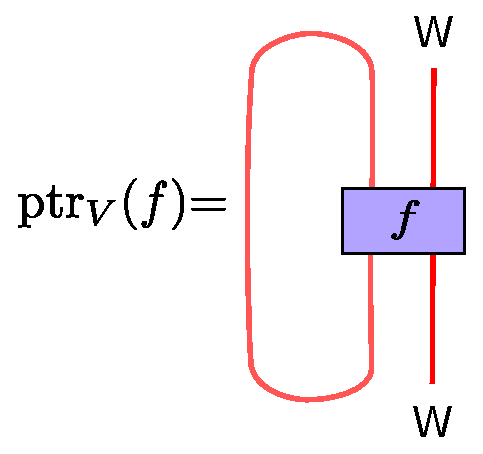
\includegraphics[width=0.25\textwidth]{ptr.eps}
\end{center}
  is a partial (pivotal) trace. If $W$ is simple, then $\ptr_V(f)=\lambda\cdot\id_W$ is a scalar, and $\tr(f)=\lambda\dim(W)$.
\end{Rem}

Working in the category $\CTR(\Vect_G^\omega)$, where formulas for the traces of braids involve sums over all the combinations of $G$-degrees of each object (subject to some condition), this will allow us to get away with one less sum (or, when coding the formulas, one less nested loop):
\begin{Rem}\label{trick}
  Let $V,W\in\CTR(\Vect_G^\omega)$ with $W$ the simple object corresponding to $(g,\chi)$, and let $f\colon V\ot W\to V\ot W$. Then $\tr_V(f)=\lambda\id$; the scalar $\lambda$ is determined by the component $\tr_V(f)|_{W_g}\colon W_g\to W_g$ of $\tr_V(f)$ by $\lambda\dim W_g=\tr(\tr_V(f)|_{W_g})$, and thus $\tr(f)=|\overline g|\tr(\tr_V(f)|_{W_g})$
\end{Rem}

As an illustration and warm-up for the calculations in \cref{sec:borr-tens-twist} we will consider the $S$-matrix for two simple objects $V,W\in\mathcal{Z}(\Vect^\omega_G)$, corresponding to the pairs $(g,\chi_1)$ and $(h, \chi_2)$. We need to compute
\begin{equation*}
  S_{(g,\chi_1),(h,\chi_2)}=\tr(\sigma_{WV}\sigma_{VW})=\tr(\sigma^2)=\tr(R(\sigma^2)),
\end{equation*}
where (no parentheses being necessary on two objects) there is no difference between the representation $R$ of the braid group $\mathbb B_2$ on one generator $\sigma$ and simply instances of the braiding of the category $\CTR(\Vect_G^\omega)$.

If we write $V = \underset{x\in \overline{g}}\oplus V_x$ and $W = \underset{x\in \overline{h}}\oplus W_y$, then for $  v\in V_x$ and $  w\in W_y$ we have
\begin{align*}
  \sigma^2(  v\ot  w)&=\sigma(x\hit   w\ot   v)\\
  &=|x {\hit}  w|\hit   v\ot x\hit   w\\
  &=(x\hit y) \hit   v\ot x\hit  w.
\end{align*}

We can endow $V\ot W$ with a $G\times G$-grading composed of the $G$-gradings of $V$ and $W$. Then
\begin{align*}
  \deg_{G\times G}\sigma^2(v\ot w)=((x\hit y) \hit x,x \hit y)
\end{align*}
for $x=|v|,y=|w|$.

For a finite group $\Gamma$, a $\Gamma$-graded vector space $E$, and an endomorphism $f$ of $E$ let $f_0$ be trivial component of $f$ with respect to the $\Gamma$-grading of $\End(E)$. Then $\tr(f)=\tr(f_0)$.

In our example, considering the $G\times G$-grading of $V\ot W$, we see that $\sigma^2( v\ot  w)$ has the same degree as $v\ot w$ if and only if $x$ and $y$ commute.

\begin{equation} \label{degree condition}
(\sigma^2)_0(v\ot w) = \begin{cases} 
          x\hit v\ot y\hit  w & [x,y]=1 \\
          0 & [x,y] \neq 1 
       \end{cases}
\end{equation}

In particular
\begin{equation*}
  S_{V,W}=\tr(\sigma^2)=\tr((\sigma^2)_0)=\sum_{\substack{x\in \overline g\\y\in\overline h\\ [x,y]=e}}\chi_1^x(y)\chi_2^y(x)
\end{equation*}
Using \cref{trick} we can replace the double sum by a single sum; also, we can use~(\cref{chi}):
\begin{align*}
S_{(g, \chi_1),(h, \chi_2)} &= |\hb|\sum_{x \in \gb}^{[x,h]=1} \chi_1^x (h) \chi_2 (x)\notag\\
%\label{Sconj}
&=|\hb| \sum_{x \in \gb}^{[x,h]=1} \alpha_{g}(c, p) \alpha_{g}\inv(p, p\inv\hit c)\chi_1(p\inv\hit c) \chi_2 (x)
\end{align*} 
where $p$ stands for any group element satisfying $p\hit g=x$. Alternatively, we can use the bijection $G/C_G(g) \rightarrow g^G$ given by $aC_G(g)\mapsto a\hit g $ to rewrite
\begin{align*}\label{Sgroup}
  S_{(g, \chi_1),(h, \chi_2)} &=\frac{|\hb|}{|C_G(g)|}\sum^{[p\hit g,h]=1}_{p\in G} \alpha_{g}(h, p) \alpha^{-1}_{g}(p, p^{-1}\hit b)\chi_1(p^{-1}\hit b) \chi_2 (p\hit g)\\
  &={|\hb|}\sum^{[p\hit g,h]=1}_{p\in G/C_G(g)} \alpha_{g}(h, p) \alpha^{-1}_{g}(p, p^{-1}\hit b)\chi_1(p^{-1}\hit b) \chi_2 (p\hit g)
\end{align*}
As mentioned, this formula is (up to conventions) quite like the formula in \cite{Coste2000FiniteGM}, except for two details: We have a single sum over one conjugacy class instead of a double sum, and we have half the cocycle (``$\alpha$'') terms due to the fact that we need to use (\cref{chi}) on only one of the two objects.

\section{The B-tensor}\label{sec:borromean-tensor}

A modular category (in fact any spherical braided fusion category) defines a numerical invariant of framed knots and links which can be written as the pivotal trace of the image in the category of a braid whose closure is the link, with its components colored by simple objects of the category. Read differently, each fixed framed link defines a numerical invariant of modular categories in this fashion. More precisely, the invariant is then indexed by as many simple objects as the link has components.

Among this infinite supply of numerical invariants (among which the $S$-matrix and, up to a dimension factor, the $T$-matrix can also be found) we pick one example, for the heuristic (and art historical) reasons cited at the beginning of this chapter.

\begin{Def}
  The borromean tensor (or $B$-tensor) of a modular category $\C$ with simples $(X_i)_{i\in I}$ is the family
  \begin{equation}
    \label{eq:borromeo}
    B_{ijk}:=\tr(B((\sigma_2\inv\sigma_1)^3)
  \end{equation}
  where $B((\sigma_2\inv\sigma_1)^3)\in\Aut_{\C}((X_i\ot X_j)\ot X_k)$. Graphically, this may be represented as 
\begin{center}
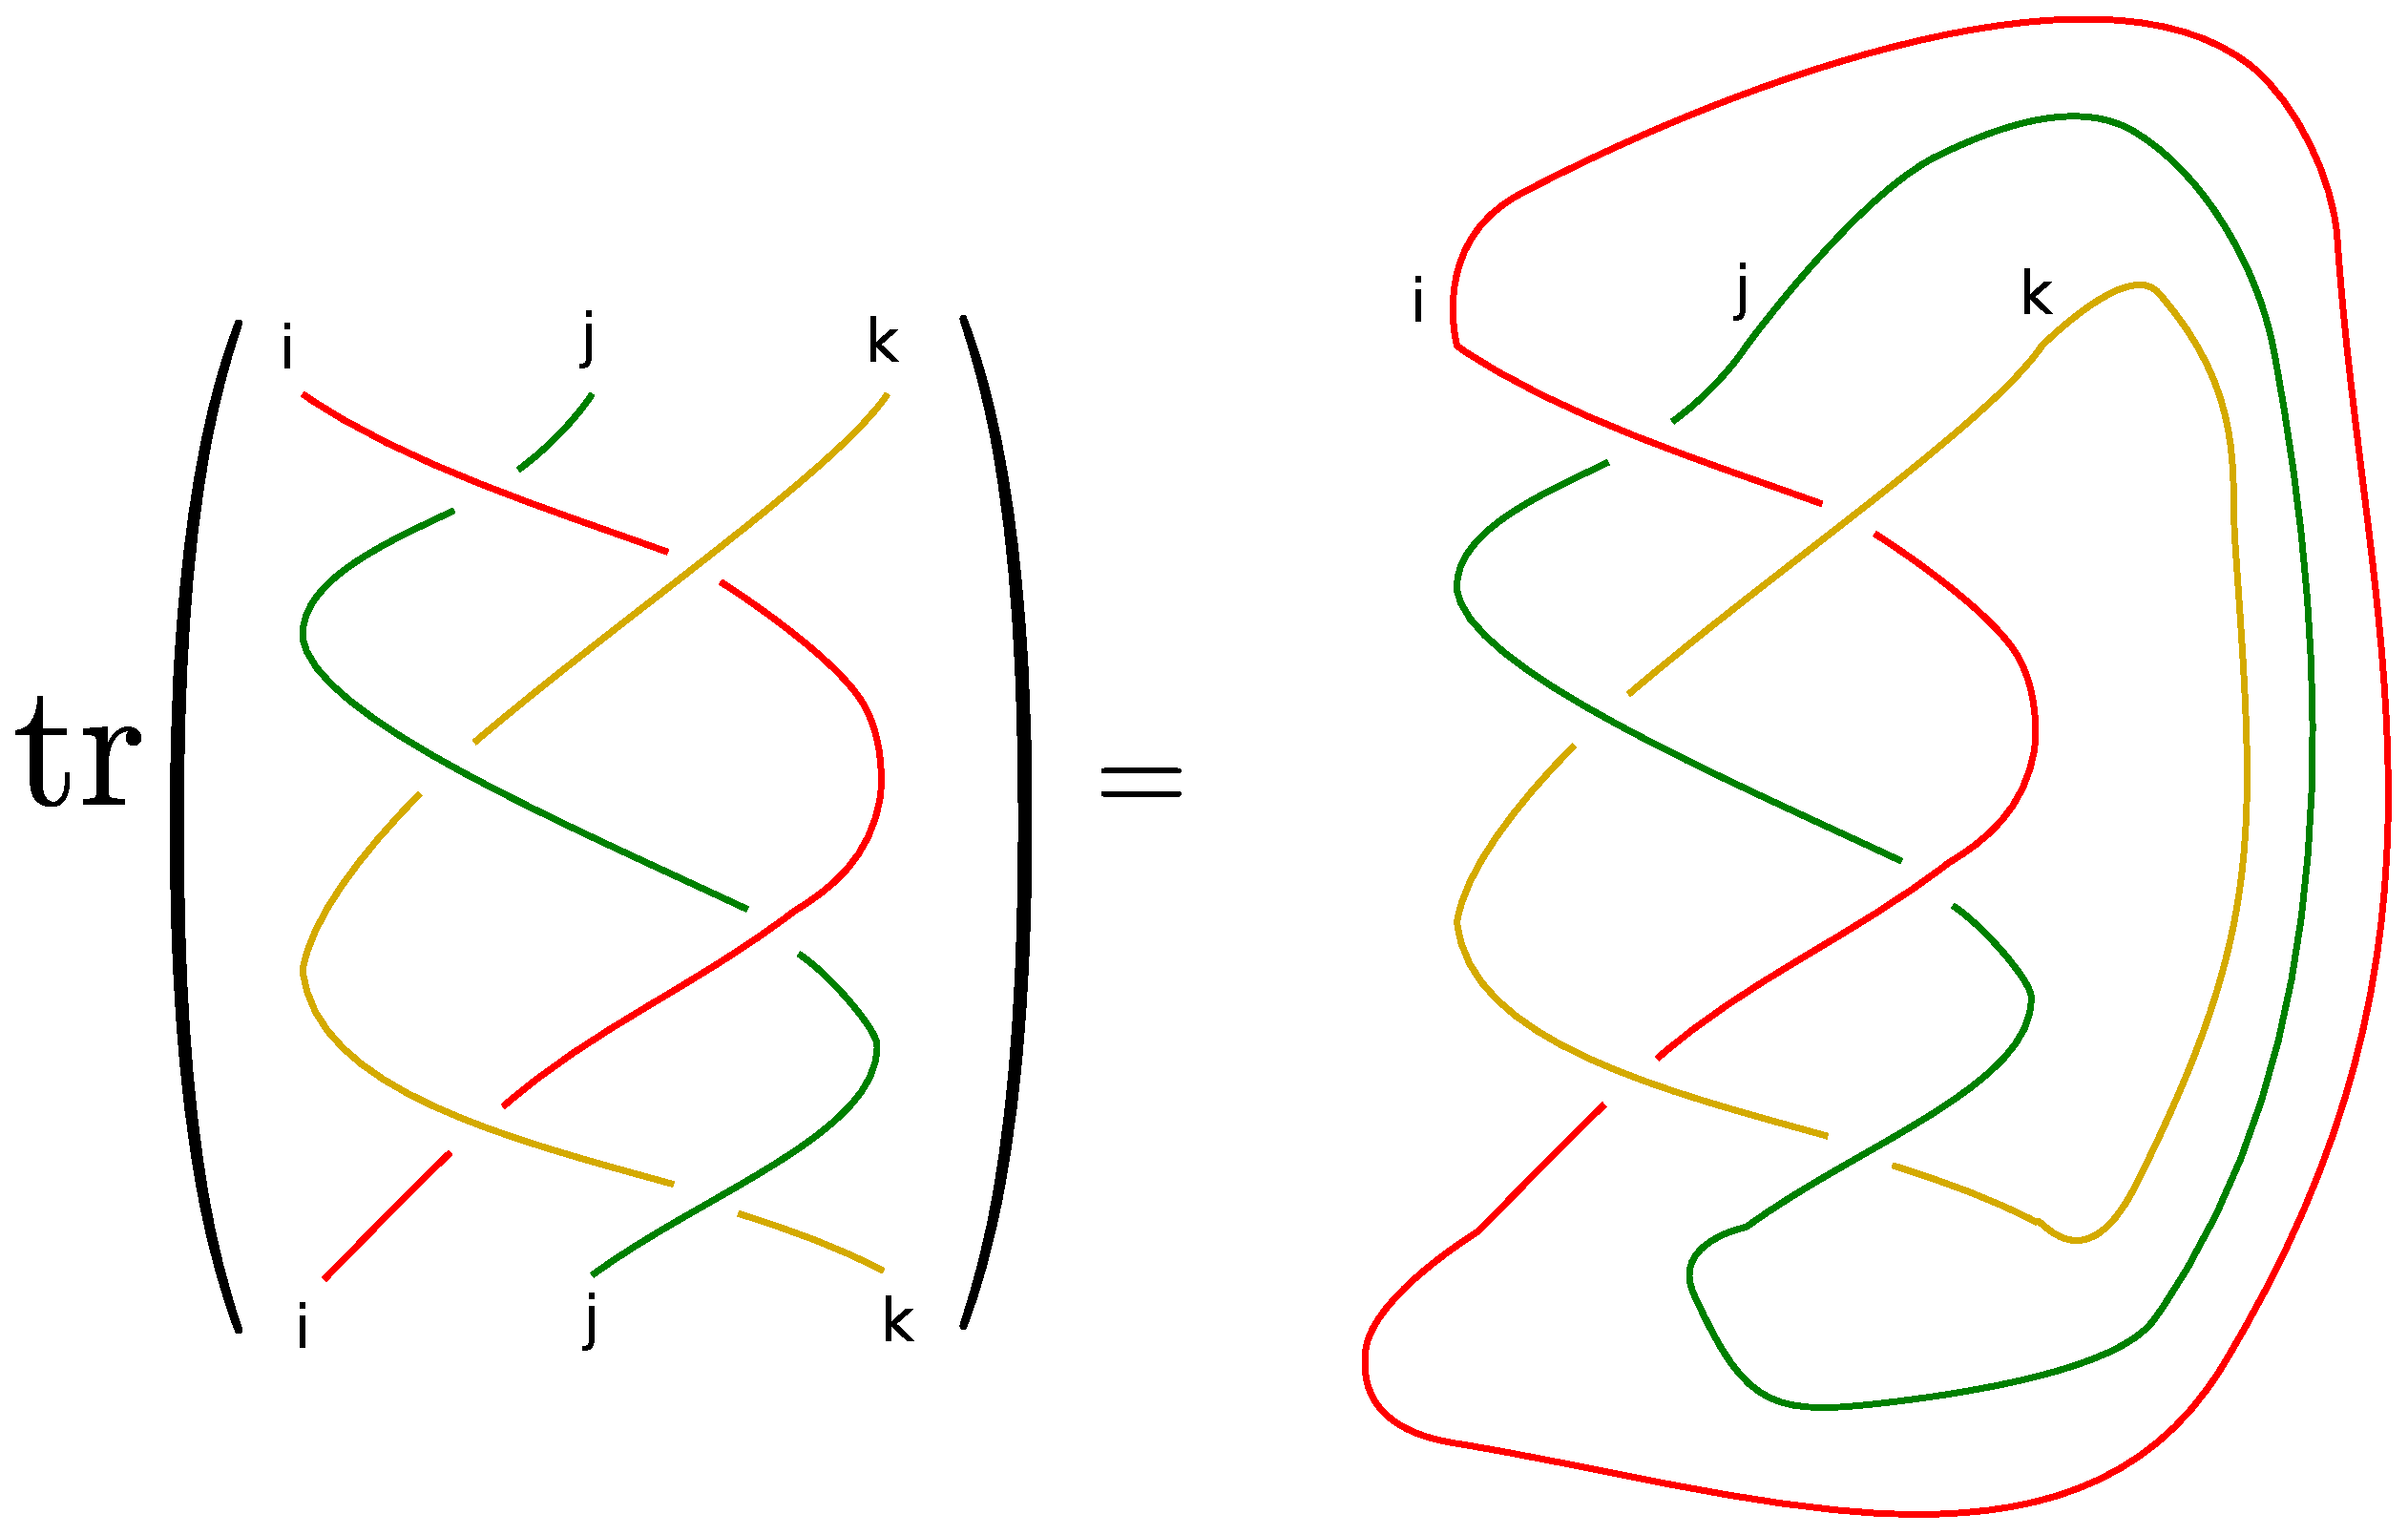
\includegraphics[width=0.4\textwidth]{b-braid.eps}
\end{center}


(In the graphical representation, we let $i$ stand for $X_i$.)
\end{Def}
\begin{Lem}
 The following equalities hold:
\begin{enumerate}
\item
$B_{ijk}=B_{jki}=B_{kij}$
\item
$B_{ijk}=B_{jik^{\ast}}$
\item
$B_{ijk}=\overline{B_{kji}}$ if $\C$ statisfies the $\mathcal F$-property (see \cite{MR2832261}).
\end{enumerate}
\end{Lem}
\begin{proof}
Clearly cyclicity of the trace implies that the $B$-tensor is invariant with respect to cyclic permutations of its three indices. We need to show the other symmetry properties:
If we conjugate the braid corresponding to the $B$-tensor by
\begin{center}
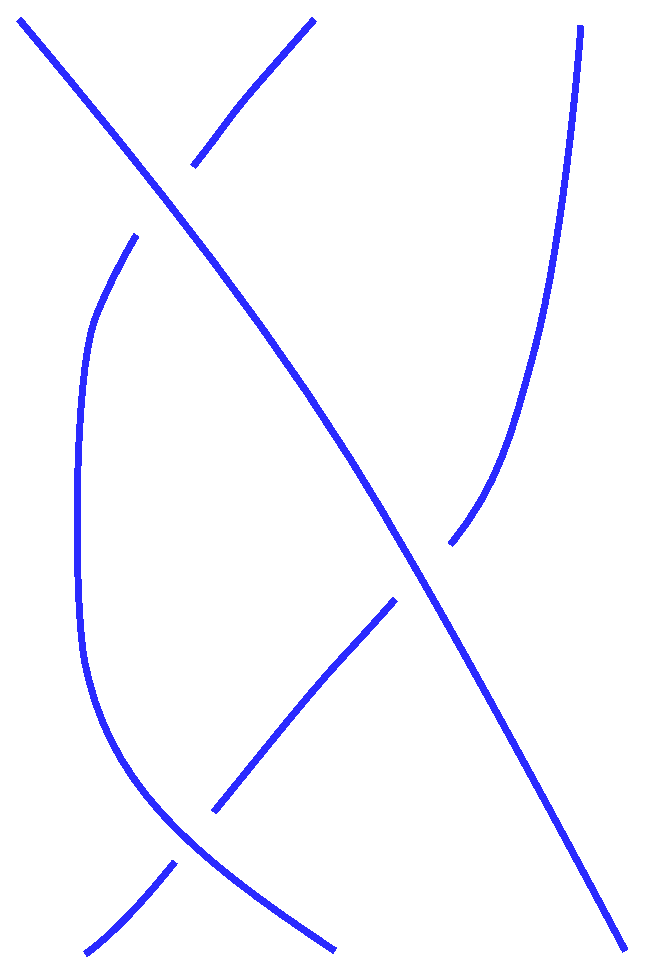
\includegraphics[width=0.08\textwidth]{conj.eps}
\end{center}
then we get that the trace of the resulting braid, 
\begin{equation}\label{conjugated}
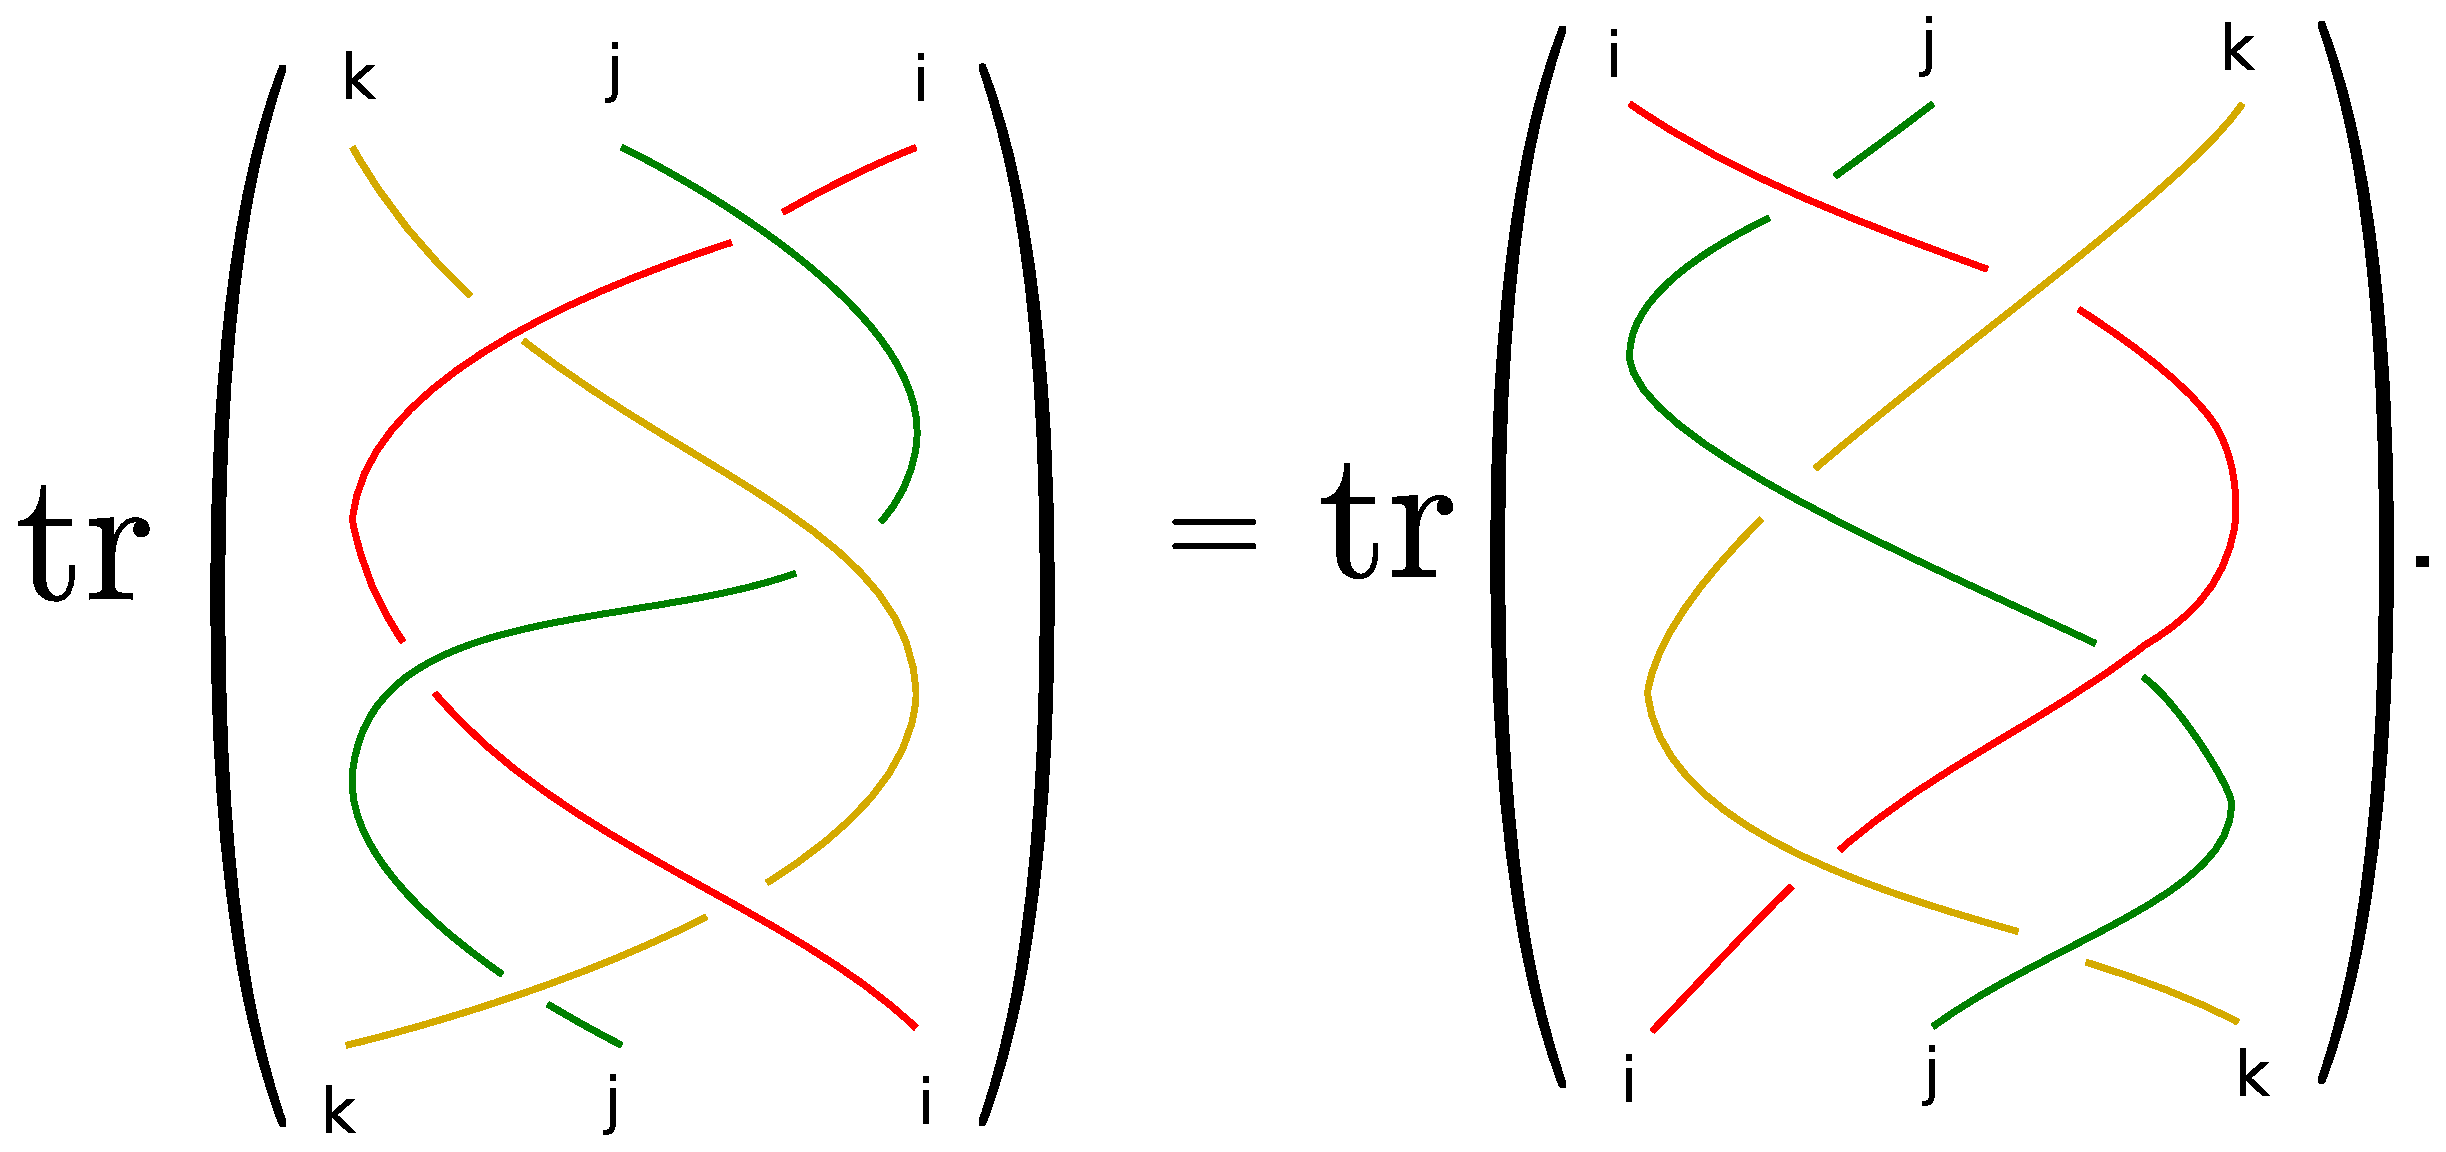
\includegraphics[width=0.5\textwidth]{conjugated.eps}
\end{equation}
 
Furthermore, we have
\begin{equation}
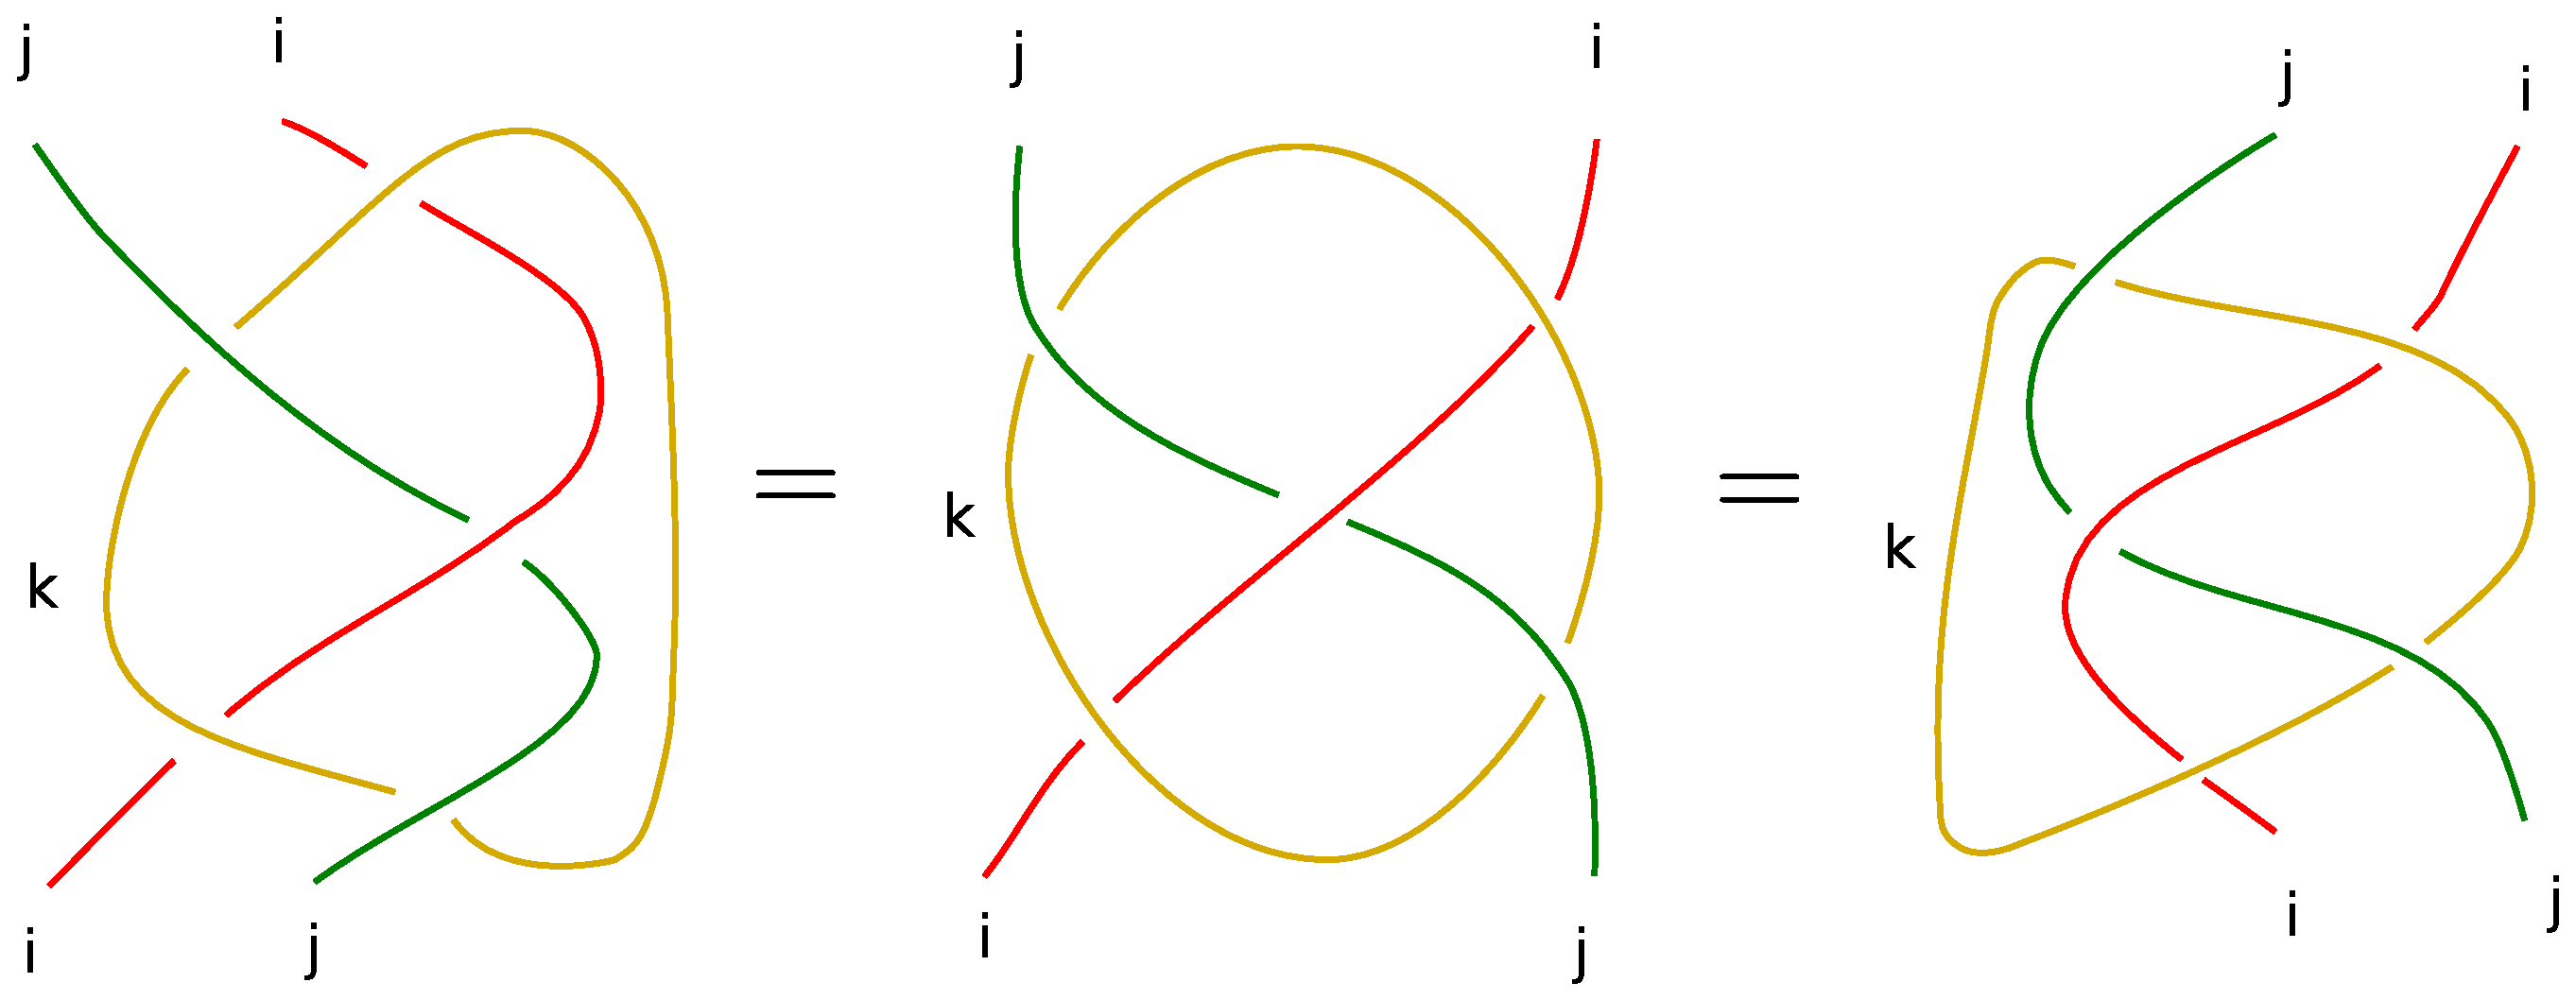
\includegraphics[width=0.7\textwidth]{slidethru.eps}
\end{equation}
and thus,
\begin{equation}
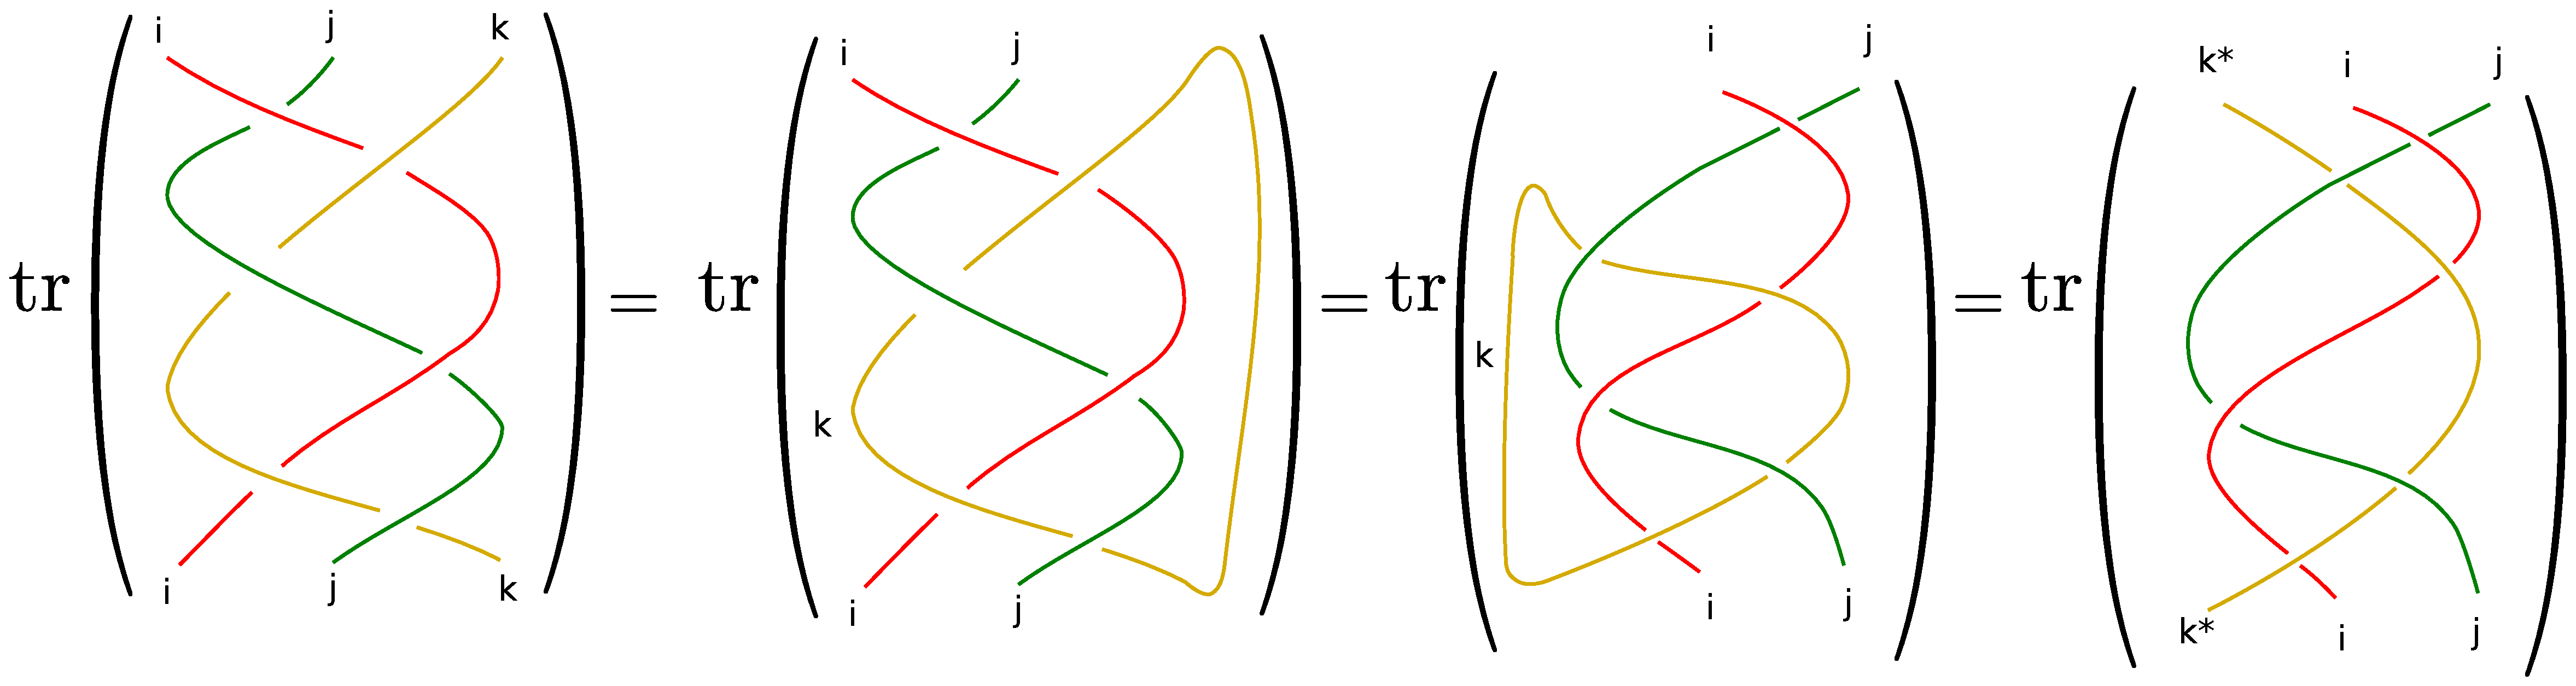
\includegraphics[width=0.9\textwidth]{final.eps}
\end{equation}
Combining with \eqref{conjugated} we see that $B_{ijk}=B_{jik^*}$. Together with the cyclic permutation invariance, this yields that $B$ is invariant under any permutation of its indices combined with dualizing an even or odd number of its indices according to the parity of the permutation. If the borromean braid has finite order in the category in question (as is the case for group-theoretical modular categories, see \cite{MR2832261}), then $B_{ijk}$ is also the complex conjugate of the trace of the inverse Borromean braid. But the left hand side of \eqref{conjugated} is that trace, so $B_{ijk}=\overline{B_{kji}}$. So in this case $B$ is invariant under permutation and dualization of its indices, up to conjugation if the number of dualized indices has the opposite parity of the permutation.
\end{proof}
For larger rank categories, these symmetry properties could serve to speed up the computation of the borromean tensor, although, truth be told, we have so far only used them to debug our code.
\section{The B-tensor of a twisted double}\label{sec:borr-tens-twist}
\newcommand\Pe{P}

In this section we will derive an explicit formula for the borromean tensor in the Drinfeld center of a pointed fusion category, in terms of the group, the cohomological data, and the projective characters parametrizing the simple objects. It should be noted that in principle it is known how to obtain such formulas for the topological invariants defined by braided monoidal categories. Nevertheless it is a rather tedious undertaking to provide them in complete detail.


Consider three simple objects $ U, V, W \in  \mathcal{Z}(Vec^\omega_G)$, parametrized by couples $(g, \chi_1)$, $(h, \chi_2)$ and $(k, \chi_3)$. Take $u\in U_x, v\in V_y,  w\in W_z$, where $x\in \gb, y\in \hb, z\in \kb$.

Looking at the $G^3$-degree of tensors in $(U\ot V)\ot W$ (which is not affected by associativity isomorphisms), we see that for $u\in U_x$, $v\in V_y$, $w\in W_z$ we have
$\deg_{G^3}(R(\sigma_2\inv\sigma_1))(u\ot v\ot w)=\Pe(x,y,z)$ if we define $\Pe\colon G^3\to G^3$ by $\Pe(x,y,z)=(x\hit y,z,z\inv\hit x)$. Note $\Pe\inv(x,y,z)=(y\hit z,y\hit z\inv\hit x,y)$. Now in order that $((\sigma_2\inv\sigma_1)^3)_0(u\ot v\ot w)\neq 0$, we need to have $\Pe^3(x,y,z)=(x,y,z)$, or equivalently $\Pe^2(x,y,z)=\Pe\inv(x,y,z)$. Comparing
\begin{align*}
  \Pe^2(x,y,z)&=\Pe(x\hit y,z,z\inv\hit x)\\
            &=((x\hit y)\hit z,z\inv\hit x,(z\inv\hit x\inv)\hit x\hit y)\\
            &=((x\hit y)\hit z,z\inv\hit x,[z\inv,x\inv]\hit y)\\
  \Pe\inv(x,y,z)&=(y\hit z,y\hit z\inv\hit x,y)
\end{align*}
we see that:
\begin{align}
  ((\sigma_2\inv\sigma_1)^3)_0&|_{U_x\ot V_y\ot W_z}\neq 0\notag\\
                            & \Leftrightarrow
                              \begin{cases}(x\hit y)\hit z=y\hit z\\
                                z\inv\hit x=y\hit z\inv\hit x\\
                                [z\inv,x\inv]\hit y=y
                              \end{cases}\notag\\
                            &\Leftrightarrow\label{eq:condition0}
                              \begin{cases}[[y\inv,x],z]=1\\
                                [[z,y],x]=1\\
                                [[z\inv,x\inv],y]=1
                              \end{cases}
\end{align}

We evaluate the morphism $R((\sigma_2\inv\sigma_1)^3)$ in three steps.
\begin{align*}
  R(\sigma_2\inv\sigma_1)&((u\ot v)\ot w)\\
                         :&=\Phi(V\ot\sigma\inv)\Phi\inv(\sigma\ot W)((u\ot v)\ot w)\\
  &=\Phi(V\ot\sigma\inv)\Phi\inv((x\hit v\ot u)\ot w)\\
  &=\Phi(V\ot\sigma\inv)(\omega(x\hit y,x,z)(x\hit v\ot(u\ot w))\\
  &=\Phi(\omega(x\hit y,x,z)(x\hit v\ot (w\ot z\inv\bhit u)\\
                         &=\omega\inv(x\hit y,z,z\inv\hit x)\omega(x\hit y,x,z)(x\hit v\ot w)\ot z\inv\bhit u\\
                         &=\psi(x,z\inv\hit x,x\hit y,z)\Psi((u\ot v)\ot w)
 \end{align*}
 with
 \begin{align*}
   \psi(x,x',y,z)&=\omega\inv(y,z,x')\omega(y,x,z)\alpha_x\inv(z,z\inv)\\
              &=\omega\inv(y,z,x')\omega(y,x,z)\alpha_{x'}\inv(z\inv,z)\\
            \Psi(u\ot v\ot w)&=(|u|\hit v\ot w)\ot |w|\inv\hit u
\end{align*}
Further
\begin{multline*}
  R(\sigma_2\inv\sigma_1)((x\hit v\ot w)\ot z\inv\hit u)\\
  =\psi(x\hit y,(z\inv\hit x)\inv\hit(x\hit y),(x\hit y)\hit z,z\inv\hit x)\Psi((x\hit v\ot w)\ot z\inv\hit u)
  \\ 
  =\psi(x\hit y,y,y\hit z,z\inv\hit x)\Psi((x\hit v\ot w)\ot z\inv\hit u)\\
\end{multline*}
where
\begin{multline*} \Psi((x\hit v\ot w)\ot z\inv\hit u)\\
  =\alpha((z\inv\hit x)\inv, x)((x\hit y)\hit w\ot z\inv\hit u)\ot [z\inv,x\inv]\hit v\\
  \in W_{(x\hit y)\hit z}\ot U_{z\inv\hit x}\ot V_{[z\inv,x\inv]\hit y}=W_{y\hit z}\ot U_{z\inv\hit x}\ot V_y.
\end{multline*}
Further,
\begin{multline*}
  R(\sigma_2\inv\sigma_1)(((x\hit y)\hit w\ot z\inv\hit u)\ot[z\inv,x\inv]\hit v)\\
  =\psi(y\hit z,y\inv\hit(y\hit z),(y\hit z)\hit(z\inv\hit x),y)\Psi((x\hit y)\hit w\ot z\inv\hit u\ot[z\inv,x\inv]\hit v)\\
  =\psi(y\hit z,z,x,y)\Psi((x\hit y)\hit w\ot z\inv\hit z\ot[z\inv,x\inv]\hit v)\\
\end{multline*}
\begin{multline*}
\Psi((x\hit y)\hit w\ot z\inv\hit z\ot[z\inv,x\inv]\hit v) \\
  =\alpha_x(y\hit z, z\inv)\alpha_z(y, x\hit y)\psi(y\hit z,z,x,y)([y,z]\hit u\ot [z\inv,x\inv]\hit v\ot[y,x]\hit w.
\end{multline*}
Thus
\begin{multline*}
  R((\sigma_2\inv\sigma_1)^3((u\ot v)\ot w)\\
  =\Omega(x,y,z)[y,z]\hit u\ot[z\inv,x\inv]\hit v\ot [y,x]\hit w
\end{multline*}
with
\begin{multline}\label{omega}
\Omega(x,y,z)=\psi(x,z\inv\hit x,x\hit y,z)\psi(x\hit y,y,y\hit z,z\inv\hit x)\psi(y\hit z,z,x,y)\\
  =\omega(x\hit y,z,z\inv\hit x)\omega\inv(x\hit y,x,z)\alpha_x\inv(z,z\inv)\\
  \omega(y\hit z,z\inv\hit x,y)\omega\inv(y\hit z,x\hit y,z\inv\hit x)\alpha_y\inv(z\inv\hit x\inv,z\inv\hit x)\\
  \omega(x,y,z)\omega\inv(x,y\hit z,y)\alpha_z(y\inv,y)
\end{multline}

We conclude that
\begin{align*}
  B&_{(g,\chi_1),(h,\chi_2),(k,\chi_3)}\\&=\tr(R((\sigma_2\inv\sigma_1)^3))\\
  &=\tr(R((\sigma_2\inv\sigma_1)^3)_0)\\
  &=\sum_{\substack{x\in\ol g,y\in\ol h,z\in\ol k\\~(\cref{eq:condition0})}}\Omega(x,y,z)\chi_1^x([y,z])\chi_2^y([z\inv,x\inv])\chi_3^z([y,x]).
\end{align*}

Using \cref{trick}, we can reduce the three summations in the preceding formula to two.
\begin{align*}
  B&_{(g,\chi_1),(h,\chi_2),(k,\chi_3)}\\
   &=|\ol k|\sum_{\substack{x\in\ol g,y\in\ol h \\~(\cref{eq:condition1})}}\Omega(x,y,k)\chi_1^x([y,k])\chi_2^y([k\inv,x\inv])\chi_3([y,x])\\
   &=|\ol k|\sum_{\substack{x\in\ol g,y\in\ol h \\~(\cref{eq:condition1})}}
  \begin{aligned}[t]
    \Omega&(x,y,k)\alpha_{g} ([y, k], p)\alpha^{-1}_{g}(p, p^{-1} \hit [y, k])\\
    &\alpha_{h}([k^{-1}, x^{-1}],q) \alpha^{-1}_{h} (q, q^{-1} \hit [k^{-1},x^{-1}])\\
    &\chi_1^x([y,k])\chi_2^y([k\inv,x\inv])\chi_3([y,x]).
  \end{aligned}
\end{align*}
with
\begin{equation}\label{eq:condition1}
  \begin{aligned}[c]
    [[k, y], x] &= 1\\
    [[y^{-1}, x],k]&=1
  \end{aligned}
\end{equation}
Finally, we can express the characters $\chi_1^x$, $\chi_2^y$ in terms of $\chi_1,\chi_2$ using (\cref{chi}):
\begin{align}
  B&_{(g,\chi_1),(h,\chi_2),(k,\chi_3)}\notag\\
   &=|\ol k|\sum_{\substack{p\in G/C_G(g)\\q\in G/C_G(g)\\~(\cref{eq:condition3})}}
  \begin{aligned}[t]\Omega(p\hit g&,q\hit h,k)(p\hit\chi_1)([q\hit h,k])\\
    &(q\hit \chi_2)([k\inv,p\hit g\inv])\chi_3([q\hit h,p\hit g])  
  \end{aligned}\\
   &=\frac{|\ol g||\ol h||\ol k|}{|G|^2}\sum_{\substack{p\in G\\q\in G
  \\~(\cref{eq:condition3})}}\label{eq:1}
  \begin{aligned}[t]\Omega(p\hit g&,q\hit h,k)(p\hit\chi_1)([q\hit h,k])\\
    &(q\hit \chi_2)([k\inv,p\hit g\inv])\chi_3([q\hit h,p\hit g])  
  \end{aligned}
\end{align}
with
\begin{equation}
\label{eq:condition3}
\begin{aligned}[c]
 [[k, q\hit h], p\hit g] &= 1\\ 
 [[(q\hit h)^{-1}, p\hit x],k]&=1.
\end{aligned}
\end{equation}
Besides the $\omega$ and $\alpha$ terms already hiding in $\Omega$, the conjugated characters in the last formulae are hiding further $\alpha$ terms from (\cref{chi}):
\begin{align*}
  (p\hit \chi_{1})([q\hit h, k]) &=\begin{aligned}[t]\alpha_{g} ([q\hit h, k], p) \alpha^{-1}_{g}(p, p^{-1} \hit [q\hit h, k])\\\cdot\chi_1(p^{-1} \hit [q\hit h, k])&
  \end{aligned}
  \\
(q\hit \chi_{2})([k^{-1}, p\hit g^{-1}])&=\begin{aligned}[t] \alpha_{h}([k^{-1}, p\hit g^{-1}],q) \alpha^{-1}_{h} (q, q^{-1} \hit [k^{-1}, p\hit g^{-1}])&\\\cdot\chi_2(q^{-1}\hit[k^{-1}, p\hit g^{-1}])&
\end{aligned}
\end{align*}


We have implemented the general formula for the $B$-tensor above in GAP; the codes are in \cref{codes}. For explicit calculations by humans, the abundance of cocycle terms (six $\omega$ terms and three $\alpha$ terms gathered in $\Omega$ plus four $\alpha$ terms hiding in conjugated projective characters) and the tedious commutation conditions on group elements certainly make the formulas somewhat unwieldy. We will now describe particular circumstances where these problems do not occur and the formula simplifies drastically. The special cases will be very useful for the key example we will treat in the following section.

\begin{Prop} Suppose there is an abelian normal subgroup $A\triangleleft G$ such that  $\omega$ is inflated from the quotient $G/A$ , and $g,h\in A$. Then
  \begin{equation}
    \label{eq:simplified}
    B_{(g,\chi_1),(h,\chi_2),(k,\chi_3)}=\vert \overline k \vert \cdot \sum_{\substack{x\in \overline g\\y\in\overline h}}\chi_1(p\inv\hit[y,k])\chi_2(q\inv\hit[k\inv,x\inv]).
  \end{equation}
  where $p\hit g=x,q\hit h=y$ in the sum. Note also that $\chi_1,\chi_2$ are ordinary characters in this case.
\end{Prop}
\begin{proof}
  The conditions are tailored to ensure that $\Omega(x,y,z)=1$ in \ref{omega}, since all values of $\omega$ where one argument is conjugate to $g$ or $h$ are trivial. The same holds for the $\alpha$ terms used in (\cref{chi}), since commutators with one element from $A$ also lie in $A$. Also, $[[k,q\hit h],p\hit g]=1$ for all $q,p$ since $q\hit h\in A$, hence $[k,q\hit h]\in A$, and $p\hit g\in A$. Finally $[q\hit h\inv,p\hit g]=1$ since $q\hit h,p\hit g\in A$ which is abelian, and in particular $[[q\hit h\inv,p\hit g],k]=1$.
\end{proof}
\begin{Cor}\label{Cor:verysimplified}
  Assume the hypotheses of the preceding corollary, and in addition that there is a subgroup $Q\subset C_G(k)$ such that $g^Q=\overline g$ and $h^Q=\overline h$. This applies for example when $G=A\semdir Q$ is a semidirect product of abelian groups. Then
  \begin{equation}
    \label{eq:verysimplified}
    B_{(g,\chi_1),(h,\chi_2),(k,\chi_3)}=\frac{\vert \ol k \vert |A|}{|C_Q(g)||C_Q(h)|} \cdot\sum_{q\in Q}\chi_2(q\hit[h,k])\chi_1(q\inv\hit[k\inv,g\inv]).
  \end{equation}
\end{Cor}
\begin{proof}
  We have bijections $Q/C_Q(g)\ni p\mapsto p\hit g\in \ol g$ and $Q/C_Q(h)\ni q\mapsto q\hit h\in \ol h$, and therefore, abbreviating $N=|C_Q(g)||C_Q(h)|$,
  \begin{align*}
    B&_{(g,\chi_1),(h,\chi_2),(k,\chi_3)}\\&=\frac{\vert\ol k  \vert}N \cdot \sum_{p,q\in Q}\chi_1(p\inv\hit[q\hit h,k])\chi_2(q\inv\hit[k\inv,p\hit g\inv])\\
                                        &=\frac{\vert\ol k  \vert}N \cdot\sum_{p,q\in Q}\chi_1(p\inv q\hit[h,q\inv\hit k])\chi_2(q\inv p\hit[p\inv \hit k\inv,g\inv])\\
                                        &=\frac{\vert\ol k  \vert}N\cdot\sum_{p,q\in Q}\chi_1(p\inv q\hit[h,k])\chi_2(q\inv p\hit[k\inv,g\inv])
  \end{align*}
  which gives the desired result after reparametrization.
\end{proof}

\section{Twisted doubles of nonabelian groups of order $pq$}\label{sec:Example}
Let $p,q$ be odd primes with $p|q-1$. There is a unique nonabelian group of order $pq$, and there are exactly $p$ inequivalent twisted doubles of that group; see \cite{2017arXiv170802796M} and below. However, these $p$ inequivalent modular categories only afford three different sets of modular data. In this section we will show that the $T$-matrix and the borromean tensor do distinguish the $p$ modular categories. We first tested this for the case $p=5$ and $q=11$ using our GAP-implementation of~(\cref{eq:1}). That is, we computed the values of $T$-matrix, $S$-matrix, and $B$-tensor in this case, and verified that no bijection between the simples of two distinct categories maps all three data to each other. Closer inspection of the experimental data also helped us pick out the particular simples to use in our borromean tensor calculations below. Thus, although no computer help is necessary in the end to prove our results, machine calculations were instrumental in  our finding them. Note that the $S$-matrix turns out not to be necessary in our example in the end; the $T$-matrix and $B$-tensor suffice.



The nonabelian group of order $pq$ where $p$ and $q$ are odd primes such that $p | q-1$ has the following presentation:
$$
\ZZ/q\ZZ \semdir \ZZ/p\ZZ \cong \langle a,b | a^q=b^p=1 ,\ bab^{-1}=a^n \rangle
$$
The integer $n \in \ZZ/q\ZZ$ must be chosen such that $n \not\equiv 1 \mod q$ and $n^p \equiv 1 \mod q$, but the group does not depend on that choice.
We note
\begin{align}\label{eq:pqformulas}
  b^k a^l b^{-k} &= a^{n^k l} &
  [a^l,b^k]&=a^{l(1-n^k)}&
  [b^k,a^l]&=a^{l(n^k-1)}
\end{align}


The canonical surjection $\ZZ/q\ZZ \semdir \ZZ/p\ZZ\to \langle b\rangle\cong\ZZ/p\ZZ$ induces an isomorphism between the cohomology groups $H^3(\langle b\rangle ,\CCu)\to H^3(\ZZ/q\ZZ \semdir \ZZ/p\ZZ,\CCu)$, where $H^3(\langle b\rangle ,\CCu)\cong \ZZ/p\ZZ$ is generated by the following cocycle $\omega$:
$$
\omega(b^i,b^j,b^k):=\exp\left( \frac{2i\pi}{p^2}([i]([j]+[k]-[j+k])\right)
$$
where $[i]\in\{0,\dots,p-1\}$ is such that $[i]\equiv i(\mod p)$.

The following is a complete list of representatives for the isomorphism classes of simples of $\CTR(\Vect_G^{\omega^u})$:
\begin{enumerate}
\item
$(1,\chi)$ where $\chi$ is an irreducible character of $G$,
\item
$(a^l,\chi_q^s)$ where $l\in (\ZZ/q\ZZ)^\times/\langle n\rangle$, $s\in\ZZ/q\ZZ$,
and $\chi_q$ is the generator of $\widehat{\langle a \rangle}\cong \ZZ/q\ZZ$ given by
$$
\chi_q(a)=\exp\left(\frac{2i\pi}{q}\right),
$$ 
\item
$(b^k,\widetilde{\chi_p^r})$ where $k\in\ZZ/p\ZZ^\times$, $r\in \ZZ/p\ZZ$, and $\widetilde{\chi_p^r}$ is the $\alpha_{b^k}^u$-projective character of $C_G(b^k)=\widehat{\langle b \rangle}$ associated to $\chi_p^r$, $\chi_p$ being the generator of $\widehat{\langle b \rangle}\cong \ZZ/p\ZZ$ given by
$$
\chi_p(b)=\exp\left(\frac{2i\pi}{p}\right).
$$ 
That is $\widetilde{\chi_p^r}=\chi_p^r \mu_{b^k}^u$ where $\alpha_{b^k}^u=d \mu_{b^k}^u$. In the sequel, we will write the simple as $(b^k,\chi_p^r)$ instead of $(b^k,\widetilde{\chi_p^r})$.
\end{enumerate}
For simplicity, we will refer to these as simples of type one, type two or type three.
\begin{Lem}\label{TLem}
The $T$-matrix of $\CTR(\Vect_G^{\omega^u})$ is given by the following:
\begin{enumerate}
\item
$\Theta(1,\chi)=1$
\item
$\Theta(a^l,\chi_q^s)=\exp\left(\frac{2i\pi}{q}sl\right)$
\item
$\Theta(b^k,\chi_p^r)=\exp\left(\frac{2i\pi}{p^2}(pkr+k^2u)\right)$, and in particular
\item $\Theta(b^k,\chi_p^r)^p=\zeta_p^{k^2u}$ for $\zeta_p=\exp(\frac{2i\pi}{p})$.
\end{enumerate}
\end{Lem}
\begin{proof}
For simples in $\CTR(\Vect_G^{\omega^u})$ of the first type, it is obvious that the corresponding twist $\Theta(1,\chi)=\frac{\chi(1)}{\chi(1)}=1$. For simples of the second type $(a^l,\chi_q^s)$, one has $\alpha_{a^l}^u=1$, and then the irreducible projective characters of the centralizer $\langle a \rangle \cong \ZZ/q\ZZ$ of $a^l$ are the usual irreducible characters. The twist is therefore given by 
$$
\Theta(a^l,\chi_q^r)=\frac{\chi_q^s(a^l)}{\chi_q^s(1)}=\exp\left(\frac{2i\pi}{q}sl\right)
$$
Finally, for simples of the last type $(b^k,\chi_p^r)$, one has $\alpha_{b^k}^u=d \mu_{b^k}^u$ where
$$
\mu_{b^k}^u(x)=\exp\left(\frac{2i\pi u}{p^2}k[\Pi(x)]\right)
$$
and $\alpha_{b^k}^u$-projective characters of the centralizer $\langle b \rangle \cong \ZZ/q\ZZ$ of $b^k$ are usual irreducible characters twisted by $\mu_{b^k}^u$. Therefore:
$$
\Theta(b^k,\chi_p^r)=\frac{\chi_q^r(b^k)\mu_{b^k}^u(b^k)}{\chi_q^r(1)\mu_{b^k}^u(1)}=\exp\left(\frac{2i\pi}{p^2}(pkr+k^2u)\right)
$$
\end{proof}

\begin{Lem}\label{BProp} The $B$-tensor of the category $\CTR(\Vect_{\ZZ/q\ZZ \semdir \ZZ/p\ZZ}^{\omega^u})$ with $p$ and $q$ odd primes such that $q|p-1$ and $u\in\{0,\dots p-1\}$ satisfies
\begin{equation}
B_{(a^l,\chi_q^s),(a^l, \chi_q^s),(b^{k}, \chi_p^r)}=p q \sum_{m=0}^{p-1} e^{\left(\frac{2i\pi sl}{q} (n^{-t}-n^t)(n^m-n^{-m})\right)};\quad 2t\equiv k(p) 
\end{equation}
\end{Lem}

\begin{proof}
We apply \cref{Cor:verysimplified} with $Q=\langle b\rangle$ and $A=\langle a\rangle$.
By \cref{eq:verysimplified} and \cref{eq:pqformulas} we have
\begin{align*}
  B_{(a^l,\chi_q^s),(a^l, \chi_q^s),(b^k, \chi_p^r)} &=pq\sum_{m=0}^{p-1}\chi_q^s(b^m \hit[a^l,b^k])\chi_q^s(b^{-m} \hit[b^{-k},a^{-l}] )\\
  &=p q \sum_{m=0}^{p-1} \chi_q^s(a^{l \cdot n^m (1-n^k)})\chi_q^s(a^{-l \cdot n^{-m} (n^{-k}-1)})\\
&= p q \sum_{m=0}^{p-1} e^{\left(\frac{2i\pi sl}{q} (n^{m}(1-n^k)+n^{-m}(1-n^{-k})\right)}.
\end{align*}
For $2t\equiv k(p)$ we get
\begin{align*}
  n^{m}(1-n^k)+n^{-m}(1-n^{-k})&\equiv n^m(1-n^{2t})+n^{-m}(1-n^{-2t})\\&=(n^{m+t}-n^{-(m+t)})(n^{-t}-n^t)
\end{align*}
so reparametrization gives the desired expression.
\end{proof}



In \cite{2017arXiv170802796M} it was shown that the $p$ non-equivalent modular tensor categories  $\CTR(\Vect_{\ZZ/q\ZZ \semdir \ZZ/p\ZZ}^{\omega^u})$ for $u=0,..,p-1$, are not distinguished by their modular data. In fact there are only three different modular data between these categories. By contrast:
\begin{Thm}\label{mainthm}
The $T$-matrix and $B$-tensor form a complete set of invariants for the $p$ non-equivalent modular categories $\CTR(\Vect_{\ZZ/q\ZZ \semdir \ZZ/p\ZZ}^{\omega^u})$ where $p$ and $q$ are odd primes such that $p|q-1$. More precisely, if there is a map $\kappa$ from the simple objects of $\CTR(\Vect_{\ZZ/q\ZZ \semdir \ZZ/p\ZZ}^{\omega^u})$ to the simple objects of $\CTR(\Vect_{\ZZ/q\ZZ \semdir \ZZ/p\ZZ}^{\omega^{u'}})$ satisfying $T_{\kappa(V)}=T_{V}$ and $B_{\kappa(U),\kappa(V),\kappa(W)}=B_{UVW}$ for all simples $U,V,W$ of the former, then $u=u'$.
\end{Thm}
\begin{proof}
  Let $\kappa$ be such a map. We will use the notations $(g,\chi)_u$ and $(g,\chi)_{u'}$ to denote simple objects of the two categories under consideration. The category corresponding to the trivial cocycle is easily distinguished from the others by the $T$-matrix alone, so we can assume $u,u'\neq 0$. Let $ls\not\equiv 0(\mod q)$. Then it is obvious from \cref{TLem} that $\kappa((a^l,\chi_q^s)_u)=(a^{l'},\chi_q^{s'})_{u'}$ with $sl \equiv s'l' \mod q$. Also, part (4) of \ref{TLem} implies that $\kappa((b^k,\chi_p^r)_u)=(b^{k'},\chi_p^{r'})_{u'}$ for some $k'$ and $r'$ with $k'^2u'\equiv k^2u(\mod p)$.

Also
\begin{align*}
B_{(a^l,\chi_q^s)_u,(a^l, \chi_q^s)_u,(b^k, \chi_p^r)_u} &= B_{\kappa((a^l,\chi_q^s)_u),\kappa((a^l, \chi_q^s)_u),\kappa((b^k, \chi_p^r))}\\
&= B_{(a^{l'},\chi_q^{s'})_{u'},(a^{l'},\chi_q^{s'})_{u'},(b^{k'}, \chi_p^{r'})_{u'}}
\end{align*}
So, with \cref{BProp} and $2t\equiv k(\mod p), 2t'\equiv k'(\mod p)$, we get
\begin{equation}\label{sumroots}
\sum_{m=0}^{p-1} \left(e^{\frac{2i\pi sl} {q} }\right)^{(n^t-n^{-t})(n^{m}-n^{-m})} = \sum_{m=0}^{p-1} \left(e^{\frac{2i\pi s'l'} {q} }\right)^{(n^{t'}-n^{-t'})(n^{m}-n^{-m})}.
\end{equation}
Since this is a $\mathbb Q$-linear relation between fewer than $q$ powers of the same primitive $q$-th root of unity $e^{\frac{2i\pi sl} {q} }=e^{\frac{2i\pi s'l'} {q}}$, we conclude that the set 
\begin{equation*}
  M_t:=\{(n^t-n^{-t})(n^{m}-n^{-m})|m=0,\dots,p-1\}\subset\ZZ/q\ZZ
\end{equation*}
is equal to the analogous set $M_{t'}$. We note that the $p$ elements $n^m-n^{-m}$ are distinct: Indeed, assume $n^m-n^{-m}=n^j-n^{-j}$ for $0\leq m,j\leq p-1$. Then
  \begin{equation*}
    0=n^m-n^j+n^{-j}-n^{-m}=(n^{-j-m}+1)(n^m-n^j).
  \end{equation*}
 Now $n^{-j-m}+1\neq 0$ since $n$ has odd order, and so $n^m=n^j$ which implies $m=j$. In particular
\begin{align*}
  \sum_{x\in M_t}x^2&=\sum_{m=0}^{p-1}(n^{t}-n^{-t})^2(n^{2m}+n^{-2m}-2)\\
                  &=(n^{t}-n^{-t})^2\left(\sum_{m=0}^{p-1}n^{2m}+\sum_{m=0}^{p-1}n^{-2m}-2p\right)\\
  &=-2p(n^{t}-n^{-t})^2,
\end{align*}
since $n^2$ and $n^{-2}$ are primitive $p$-th roots of unity in $\ZZ/q\ZZ$
and so the sum over all their powers gives zero. By the same reasoning
\begin{equation*}
  \sum_{x\in M_t}x^2=\sum_{x\in M_{t'}}x^2=-2p(n^{t'}-n^{-t'})^2
\end{equation*}
Thus $(n^t-n^{-t})^2=(n^{t'}-n^{-t'})^2$, which implies $n^t-n^{-t}=n^{t'}-n^{-t'}$ or $n^t-n^{-t}=n^{-t'}-n^{t'}$. As we have seen, this implies $t\equiv t'$ or $t\equiv -t'$ in $\ZZ/p\ZZ$. Therefore $k^2=k'^2$ and we can conclude that $u=u'$.
\end{proof}

\begin{Rem}
  There is an action of the absolute Galois group of abelian extensions  of the rationals $\Gamma:=\Gal(\Q^\ab/\Q)$ on the set of simples of any integral modular category; see \cite[Appendix]{EtiNikOst:FC}. In the case of $\CTR(\Vect_G^\omega)$ it satisfies $S_{\gamma(i),\gamma(j)}=\gamma^2(B_{i,j})$ for any $\gamma\in\Gamma$, and also $T_{\gamma(i),\gamma(i)}=\gamma^2(T_{ii})$ as shown in  \cite{MR3435813}. If we analyze the proof in \cite{2017arXiv170802796M} that the twisted doubles of nonabelian groups of order $pq$ share only three different sets of modular data, we can conclude from our result that the analogous property $B_{\gamma(i),\gamma(j),\gamma(k)}=\gamma^2(B_{ijk})$ is not satisfied. 
\end{Rem}

\section{Square-free groups and their twisted doubles} % (fold)
\label{sub:twisted_doubles_of_square-free groups}
% subsection twisted_doubles_of_square (end)
Groups of square-free order (or simple square-free groups) have been classified over a century ago by H\"older\cite{Hoelder1895}. We will briefly describe their structure and classification, and also study the structure of their twisted doubles.

For a square-free group $G$ order $|G| = \prod_{i=1}^z p_i$, where $p_i$ are distinct primes such that $p_i <p_{i+1}$, H\"older gave a formula for the number of isomorphic groups of a given order. We however use an algorithmic approach to calculate the number of square-free groups of a given order.\\ 

For a finite group $G$ such that $|G| = \prod_{i=1}^z p_i$, there exists a Sylow $p_i$-subgroup for each $p_i$, and a choice of $p_i$-Sylow subgroups, each corresponding to a prime factor $p_i$, is called a \textit{Sylow basis} for $G$. We will assume that for any such group $G$ we have already picked a Sylow basis. Let $g\hit h = ghg\inv$ for $g, h \in G$. Any square-free group can be presented in the following way,  
\begin{equation}\label{presentation}
	G= <a_i (1\leq i\leq z)| a_i^{p_i} =1, a_j\hit a_i = a_i^{n_{ij}} (1\leq j<i\leq z)>
\end{equation}
where $n_{ij}$ is referred to as the action of $a_j$ on $a_i$ which satifies \begin{equation}\label{act-condition}
	n_{ij}^{p_j}\equiv 1 \mod p_i.
\end{equation} For each pair $(p_i, p_j)$ such that $p_j|p_i-1$ and $n_{ij}$ is non-trivial, the solutions of the equation (\ref{act-condition}) form a cyclic group $<N_{ij}>$ of order $p_j$.
If $(p_i, p_j) $and $(p_j, p_t)$ are two such pairs, the element $a_j\hit a_i = a_i^{n_{ij}}$ can be conjugated by $a_t$ to obtain \begin{equation*}
	a_j^{n_{jt}}\hit a_i^{n_{it}} = a_i^{n_{ij}n_{it}}
\end{equation*}
and since $a_j^x\hit a_i^y = a_i^{yn_{ij}^x}$, we get the condition \begin{equation*}
	a_i^{n_{ij}n_{it}} = a_i^{n_{it}n_{ij}^{n_{jt}}} \implies n_{ij}^{n_{jt} -1} \equiv 1 \mod p_i
\end{equation*}
so either \begin{equation}\label{non-cont}
	n_{ij} \equiv 1 \mod p_i \quad \text{or}\quad n_{jt} \equiv 1 \mod p_j.
\end{equation} From now on, we will abuse language and say that a prime factor $p_j$ ``acts'' on a prime factor $p_i$, or equivalently that $p_i$ is ``acted upon" by $p_j$, when we mean that the subgroup $C_{p_j}$ in the Sylow basis acts non-trivially on the subgroup $C_{p_i}$ in the Sylow basis. The condition (\ref{non-cont}) means that every prime factor can either act or be acted upon, or neither, but not both. If we specialize to $i = z$ then a choice like $n_{zj} =N_{zj}^w$ , for  $w>1$, can be turned into $n_{zj} =N_{zj}$ by picking a different generator $a_j'= a_j^w$. In fact, we can assume that \begin{equation}\label{possible}
	\text{ if $n_{ij} =1$ for $i= z, z-1,\dots z-r$ then $n_{ij}= 1$ or $N_{ij}$ for $i = z-r-1$.}
\end{equation} 
The existence of groups with presentation (\ref{presentation}) and conditions (\ref{act-condition}), (\ref{non-cont}) and (\ref{possible}) is shown in the text \cite{MR896269}. \begin{Prop}\label{uniqueness}
Two presentations of type (\ref{presentation})  with conditions (\ref{act-condition}), (\ref{non-cont}) and (\ref{possible}) that differ in one of the exponents $n_{ij}$ give non-isomorphic groups (for $z>1$).
\end{Prop}
We need a small lemma before we prove this.
\begin{Lem}[Hall]\label{hall}
If $A$ is a finite solvable group of order $uv$ and $(u,v) = 1$, then there is at least one subgroup of order $u$ and any two such subgroups are conjugate.
\end{Lem}
\begin{proof}[Proof of Proposition \ref{uniqueness}]
Consider two groups $G$ and $G'$ of type (\ref{presentation}) with generators $a_i$ and $a_i', (1\leq i \leq z)$, obeying conditions (\ref{act-condition}), (\ref{non-cont}) and (\ref{possible}). 
In order to use an inductive argument, let the proposition be true for groups with $z-1$ generators. Let $n_{ij}\neq n'_{ij}$ for some $j< i$. 
If $i< n$ then $<a_1,a_2,\dots, a_{z-1}> \not\cong <a'_1,a'_2,\dots, a'_{z-1}>$, and so $G\not\cong G'$. Now if $n_{ij} = n'_{ij}$ for $1\leq i<j<z$, and if $n_{z1}\neq n'_{z1}$ then one of them is 1 and the other is $N_{z,1}$ by (\ref{possible}). so $<a_1, a_z> \not \cong <a'_1, a'_z>$, and by Lemma \ref{hall} $G\not\cong G'$. So assume that $n_{z1} = n'_{z1}$ and let $i$ be the smallest index such that $n_{z i}\neq n'_{zi}$ and assume $n'_{z i}\neq 1$, by (\ref{non-cont}) $n_{ij} = n'_{ij}=1$ for all $j<i$. If $n_{z j} = n'_{zj} = 1$ for all $j<i$ then $n_{zi} = 1$ and $n'_{zi} = N_{zi}$. Hence $<a_1, a_i, a_n>$ is abelian while $<a'_1, a'_i, a'_n>$ is not, so $G\not\cong G'$. Else, let $j$ be the smallest index such that $n_{zj} = n'_{zj} \neq 1$. Then by (\ref{possible}), $n_{zj} = n'_{zj} = N_{zj}$, so $<a'_j, a'_i, a'_z>$ has actions $N_{zj}, N_{zi}^w$ for $w \mod p_i$ whereas $<a_j, a_i, a_z>$ is either also of this type with actions $N_{zj}, N_{zi}^{w\prime}$ where $w'\not\equiv w \mod p_i$ or has $<a_i, a_z>$ abelian. Thus $G\not\cong G'$. 
\end{proof}
Let $G$ be a finite group of odd square-free order $pq$, where $q$ denotes the order of the maximal abelian normal subgroup $N \cong \ZZ_q$, and let $P$ denotes a set of generators for cyclic groups in the Sylow basis of $G$ corresponding to the prime factors of $p$, $\{p_1,\dots, p_k\}$ and $Q$ a set of generators for cyclic groups in the Sylow basis of $G$ corresponding to the prime factors of $q$, $\{q_1,\dots, q_l\}$. 
\begin{Rem}\label{chinese}
For an element $a\in Q$, the actions of any two non-trivially acting elements of $P$ generate cyclic groups of coprime order, and so by the Chinese remainder theorem we may denote the action by a single number $n_a$ whose order mod $q_a$ is the product of all $p_j\in P$ such that $b_j$ acting non-trivially on $a$. Again by the Chinese remainder theorem, there is a unique $n$ mod $q$ such that for each $a \in Q$, $n\equiv n_a \mod q_a$ where $q_a$ denotes the order of $a$. We call this $n$ the `action' associated with $G$ for obvious reasons, and along with $p$ and $q$ it determines the group (up to isomorphism).
\end{Rem}
For brevity, we may sometimes denote the group as \begin{equation}
	G = G_{p,q,n}
\end{equation}where $n$ is the action on $\ZZ_q$ by $\ZZ_p$, as described in the previous remark.\\
Given $p,q$ such that $pq$ is odd square-free, it is possible to count the number of non-isomorphic groups of order $pq$. We calculate this number explicitly for two cases.\\
Suppose $p,q$ are primes. Picking generators for the two cyclic subgroups in the Sylow basis $<a>$ of order $q$, and $<b>$ of order $p$ such that $b\hit a=a^n$, since $a = b^p\hit a = a^{n^p}$, we must have\begin{equation}
	n^p\equiv 1 \mod q.
\end{equation} If $p|q-1$, the solutions to this equation mod $q$ form a cyclic subgroup $<N>$ of order $p$. Thus we have $p$ different choices of the action $b\hit a$, the trivial one corresponding to the abelian group of order $pq$, and the remaining $p-1$ non-trivial actions turn out to give the same group up to isomorphism. Given presentations \begin{equation}
	<a, b | b^p, a^q, bab\inv = a^{N^t}>\quad \text{and} \quad <a, b | b^p, a^q, bab\inv = a^N>,
\end{equation}
we can replace the generator $b$ on the left  by $b^t$, to obtain a presentation of the form on the right. So there are two non-isomorphic groups of order $pq$ if $p|q-1$, else there is only one.

Now suppose $G$ has order $pqr$, where $p, q, r$ are prime. If we declare a condition like $p_j|p_i-1$, then we will want to know how many new groups emerge, and so we will consider a non-trivial action of the generator $a_j$ on $a_i$, because otherwise we end up with a known case. For example in the previous case, the abelian group of order $pq$ was known without imposing $p|q-1$.\\
\begin{enumerate}
	\item If $p\nmid q-1, p\nmid r-1$, and $q\nmid r-1$ there is only one possibility, the abelian group of order $pqr$. 
	\item If $p|q-1, p\nmid r-1, q\nmid r-1$, ( or if $p\nmid q-1, p| r-1, q\nmid r-1$) then the only new possibility is the direct product of the cyclic group of order $r$ (of order $q$) with the non-abelian group of order $pq$ (of order $pr$). 
	\item If $p|q-1,p|r-1, q\nmid r-1$, then using criterion (\ref{possible}) we find that there is only one non-trivial choice for the action on the factor $C_r$, $n_{rp} = N_{rp}$ and subsequently, $p-1$ distinct choices of the action corresponding to elements of $<N_{qp}>$. Hence there are $p-1$ new groups.	
\item If $p|r-1, q|r-1, p\nmid q-1$ then for both actions, there is only one non-trivial choice, so there is only one new group.
\item If $p|q-1, p|r-1$ and $q|r-1$, then either $n_{rq}$ or $n_{qp}$ is trivial, so our analysis breaks up into two cases. If $n_{rq}$ is trivial thisis equivalent to the case $p|q-1, p|r-1, q\nmid r-1$, and if $n_{qp}$ is trivial this is equivalent case $p|r-1, q|r-1, p\nmid q-1$. This yields no new groups.\\
\end{enumerate}
Such an analysis could be done for a group of any square free order, simply by studying the possible actions. In the appendix, we have provided a GAP function which takes an input a square-free number $x$, and returns the number of non-isomorphic groups of order $x$, using an algorithm described in \cite{MR506898}. 

 For groups of a given square free order 
\begin{equation}\label{order}
	p_1p_2\dots p_kq_1q_2\dots q_l,\end{equation} 
  where the $p_j$'s are the acting factors, and the $q_i$'s are either acted upon or form a central subgroup, writing
 \begin{equation}
  	p_1p_2\dots p_k;q_1q_2\dots q_l,
  \end{equation} determines a class of square-free groups, all of which have a maximal abelian normal subgroup of order $q_1q_2\dots q_l$. H\"older refers to this class as a \textit{Gattung}, German for `genus'. 	 
  Now suppose a group $G$ belongs to the \textit{Gattung} represented by 
  \begin{equation}
  	p_1p_2;q_1q_2
  \end{equation}
and suppose that in $G$, $p_1$ acts non-trivially on $q_1$ while $p_2$ acts non-trivially on both $q_1$ and $q_2$. This may be denoted in the following way,
\begin{equation}\label{arten}
	\overbracket{p_1{\underbracket{\underbracket{p_2;q_1}q_2}}} 
\end{equation}
where a specific bracket denotes action of the prime factor from which it starts, on  the prime factor at which it ends, read left to right. Note that every prime factor $p_i$ must have at least one bracket starting from it, otherwise it is possible to consider it as a constituent of the normal subgroup, thus contradicting the fact that the largest abelian normal subgroup has order $q_1\dots q_l$. The group $G$ is surely not determined by the expression (\ref{arten}) as there may be several choices of the actions indicated. The expression thus represents a class of groups, which H\"older calls an \textit{Art} (plural \textit{Arten}), German for `species'. Every \textit{Gattung} consists of several \textit{Arten}, and every \textit{Art} consists of groups with the same acting and acted upon prime factors but different actions. In fact, we will see that two groups with equivalent twisted doubles must lie in the same \textit{Art}.

We are interested in studying Drinfeld centers of pointed fusion categories $\Vect^\omega_G$, denoted $\CTR(\Vect^{\omega}_{G})$, where $G$ is a square-free group. We will henceforth not distinguish between a simple object in $\CTR(\Vect^{\omega}_{G})$ and the couple $(g, \chi)$ representing its isomorphism class (see \ref{CenterVecOmegaG}).

Apart from the trivial element, every element of $G$ is conjugate to an element of one of the following 3 types.\begin{enumerate}
\item $a_1^{g_1}\dots a_m^{g_m}$ for $a_1,\dots , a_m\in Q$ and each $g_i \in \ZZ_{q_i}^\times/<n_{a_i}> $ where $q_i$ is the order of the corresponding $a_i$ and and $<n_{a_i}>$ is the subgroup generated by the non-trivial action of $\ZZ_p$ on $a_i$.
\item $ b_1^{h_1}\dots b_n^{h_n} $ for $b_1,\dots , b_n\in P$ and $h_j \in \ZZ_{p_j}^\times$ where $p_j$ is the order of $b_j$. 
\item $ a_1^{g_1}\dots a_m^{g_m}b_1^{h_1}\dots b_n^{h_n} $ such that $a_1,\dots , a_m, b_1,\dots , b_n $ commute with each other. \end{enumerate}
No two distinct elements of type (2) are conjugate because $a_i^{g_i}\hit b_j^{h_j}$ leaves the power of $b_j$ unchanged for any $a_i \in Q$. Products of non-commuting generators are accounted for as follows. For $a \in Q$ and $b\in P$, consider an element $a^gb^h \in G$ such that $bab\inv = a^t$. Then $a^rb^ha^{-r} = a^{r(1-t^h)}b^h$. If we rewrite $g= r(1-t^h)$ for $t^h\neq 1$, so that $r =g(1-t^h)\inv$ mod $\qb$(the order of $a$), we have $a^gb^h = a^{g(1-t^h)\inv}b^ha^{-g(1-t^h)\inv}$, and we see that every such element is conjugate to $b^h$. More informally, for an element of the type $ a_1^{g_1}...a_m^{g_m}b_1^{h_1}...b_n^{h_n} $ such that some of the generators do not commute, we can simply ignore the non-commuting $a_i$'s to arrive at a representative of type (2) or (3).
\begin{Rem}\label{char}\rm As any representative $r= a_1^{g_1}...a_m^{g_m}b_1^{h_1}...b_n^{h_n}$ is comprised of commuting generators, the elements $a_1,...,a_m,b_1,...,b_n$ generate an abelian subgroup  $H\subseteq C_G(r)$. Suppose that  an  element $x\in C_G(r)$ does not commute with an element in $H$, then it must act non trivially on atleast one of its generators, say it acts on $a_1$ as $x\hit a_m = a_m^t$. Then $x\hit r = a_1^{g_1}...a_m^{tg_m}b_1^{h_1}...b_n^{h_n}$. Since all the generators of $H$ commute, $x\hit r \neq r$  and hence $x$ cannot lie in $C_G(r)$, which contradicts our earlier assumption. This tells us two things: first, $H$ is central in $C_G(r)$, and consequently normal, and secondly, elements $y, y' \in C_G(r)\backslash H = K$  are words in generators of the quotient group $G/H$ that commute with all the generators of $H$. Moreover, $H\cap K = 1$ because the two subgroups have no elements in common.  We conclude that $C_G(r)= K\times H$. \\
By the multiplicativity of characters over direct products of groups,  for an irreducible character $\chi_1$ of $C_G(r)$, \begin{equation}
	\chi_1|_{H} = \chi_1(1)\varphi^v
\end{equation} where $\varphi$ is a generator of $\hat{H}$, the group of characters on $H$, and $v$ is an integer mod $|H|$.\end{Rem}


We now give formulae for certain $T$ matrix entries which will be useful later. For an element $a\in Q$ of order $\qb$, pick a generator $\varphi$ for the cyclic group of characters of $H=<a>$, the cyclic group generated by $a$, such that for a character $\chi_1$ of $C_G(a^g)$, $\chi_1|_{<a>} = \chi_1(1)\varphi^v$, for  some integral power $v$ defined mod $\qb$. Then,
 \begin{equation}\label{a}
	  \Theta(a^{g}, \chi_1) = \frac{\chi_1(a^{g})}{\chi_1(1)}
	= \frac{\chi_1(1)\varphi^v(a^{g})}{\chi_1(1)} 
	= \exp(\frac{2\pi iv g}{\qb}).
	\end{equation}
 Similarly, for an element $b\in P$ of order $\pb$, pick a generator $\psi$ for the cyclic group of characters of $H'=<b>$, the cyclic group generated by $b$, such that for a character $\chi_2$ of $C_G(b^h)$, $\chi_2|_{<b>} = \psi^w$, for some exponent $w$ defined mod $\pb$. Then we get
 \begin{equation}
	 \Theta(b^{h}, \chi_2) = \tilde{\chi}_2(b^{h})\mu^u_{b^h}(b^h),
	 \end{equation}
where $\mu^u_{b^h}$ is a 1-cochain, such that the multiplier of the projective character $\chi_2$, $\alpha_{b^k}^u = d\mu^u_{b^h}$. When the multiplier is a coboundary, the projective character is a scalar multiple of $\tilde{\chi}_2$, an ordinary character.  The quantity $\mu^u_{b^h}$ is defined as \begin{equation}
	\mu_{b^h}^u (b^r) = \exp(\frac{2\pi iu}{\pb^2}[h][r]),
\end{equation}
where $[-]$ denotes that the number is taken mod $\pb$. So finally,
\begin{equation}
	 \Theta(b^{h}, \chi_2)	 = \frac{\chi_2(1)\varphi^w (b^{h})\mu^u_{b^h}(b^h)}{\chi_2(1)} 
	 =\exp (\frac{2\pi iwh}{\pb} + \frac{2\pi i}{\pb^2}[h]^2u).
\end{equation}



\section{The S matrix for twisted doubles of square-free groups}
In this section, we state and prove a theorem that gives necessary and sufficient conditions for when certain diagonal S-matrix entries of two twisted doubles of square-free groups can be equal. For $a\in Q$ of order $q_a$, let $P_a = \{b_1,\dots,b_z\}$  be the set of generators which act non-trivially on $a$, with actions $n_1,\dots, n_z$ and orders $\pb_1,..., \pb_z$, with $p_a$ the product of these orders. 
\begin{theorem}
For two square-free groups of odd order $pq$, \begin{equation}
	G = G_{p,q,n} \quad \text{and} \quad G'=G_{p,q,n'}
\end{equation} where $n$ and $n'$ are distinct modulo $q$ and coprime to $p$, the twisted doubles $\CTR(\Vect_{G_{p,q,n}}^\omega)$ and $\CTR(\Vect_{G_{p,q,n'}}^{\omega'})$, will give the same diagonal S-matrix entry for objects $(a^g, \chi_1)$ and $(a^{g'}, \chi_1')$ for $a \in Q$,  if and only if \begin{equation}
	gv = g'v', \quad n^{\prime} \equiv  n^{\pm 1} \mod \qb, \quad \text{and}\quad \chi_1(1)=\chi'_1(1).
\end{equation}
where $v,v'$ are such that $\chi_1|_{<a>} = \chi_1(1)\varphi^v$ and $\chi_1'|_{<a>}= \chi_1(1)\varphi^{v'}$ for a chosen generator $\varphi$ of the group of characters of $<a>$, and $q_a$ denotes the order of $a$.
\end{theorem}
\begin{proof}
We have the following formula for entries of the diagonal S-matrix corresponding to $(a^g, \chi_1)$, (see [KMS] for a general formula)
\begin{equation}
	S_{(a^g, \chi_1)(a^g, \chi_1)} = |\overline{a^g}| \sum_{x\in G/C_G(a^g)}^{[x\hit a^g, a^g] = 1} \alpha_{a^g}(a^g, x)\alpha_{a^g}(x, x^{-1}\hit a^g)\chi_1(x^{-1}\hit a^g)\chi_1(x\hit a^g)
\end{equation}
where $|\overline{a^g}|$ denotes the order of the conjugacy class represented by $a^g$ and $\alpha_{a^g}$ is a 2-cocycle on $G$ determined by the associator $\omega$, the general formula being
\begin{equation}\label{2cocycle}
 	\alpha_h(x, y) = \omega(x, y, h)\omega\inv(x, y\hit h, h )\omega(xy\hit h, x, y),
 \end{equation} for $h, x, y \in G$, where $\hit$ denotes the left action by conjugation. Since the elements that are not in $C_G(a^g)$ are elements of $P$ that act on $a^g$, (denote them by $b_1,\dots,b_y$ of order $\pb_1,\dots,\pb_y $ respectively) we have
\begin{align}  
S(a^g, \chi_1)(a^g, \chi_1) &=  \frac{\qb-1}{p_a}\sum_{h_1=0}^{\pb_1}...\sum_{h_y=0}^{\pb_y}\chi_1(b_1^{-h_1}...b_y^{-h_y}\hit a^g)\chi_1(b_1^{h_1}...b_y^{h_y}\hit a^g)\nonumber\\
&=\chi_1(1)^2\frac{\qb-1}{p_a}\sum_{h_1=0}^{\pb_1}...\sum_{h_y=0}^{\pb_y}\varphi^v (a^{gn_1^{-h_1}\dots n_z^{-h_z}})\varphi^v( a^{gn_1^{h_1}\dots n_y^{h_y}})\nonumber\\
&=\chi_1(1)^2\frac{\qb-1}{p_a}\sum_{h=0}^{\pb_1...\pb_y}\exp(\frac{2\pi i}\qb gvh(n_a^{-h} +n_a^h))
\end{align}
Notice that there are no $\alpha$ terms in the above expression, for one can always choose $\omega$  in \ref{2cocycle} such that it is inflated from the quotient $G/\ZZ_q$. In particular, the value of $\omega$ is trivial if one of its arguments is an element of $\ZZ_q$.
In the last equality, we denote the action of $\ZZ_p$ on $a$ by $n_a$ following Remark (\ref{chinese}).  Since $n\equiv n_a\mod \qb$, we can write

\begin{equation}
	S(a^g, \chi_1)(a^g, \chi_1) =\chi_1(1)^2\frac{\qb-1}{p_a}\sum_{h=0}^{\pb_1...\pb_y}\exp(\frac{2\pi i}\qb gvh(n^{-h} +n^h))
\end{equation}
Consider two categories $\mathcal{Z}(\text{Vec}^{\omega^{u}}_{G_{p,q,n}})$ and $\mathcal{Z}(\text{Vec}^{\omega^u}_{G_{p,q,n'}})$ which give rise to the same modular data. Consider a fixed bijection between simples of $\mathcal{Z}(\text{Vec}^{\omega^u}_{G_{p, q, n}})$ and $\mathcal{Z}(\text{Vec}^{\omega^{u'}}_{G_{p,q,n'}})$, that preserves the modular data.  Recall that $n\equiv n_a \mod \qb$, where $\qb$ is the order of $a$. Comparing the diagonal entries of the $S$ matrices, $S(a^g, \chi_1)(a^g, \chi_1)$ and $S(a^{g'}, \chi_1')(a^{g'}, \chi_1')$ computed above,
\begin{equation}
 	\chi_1(1)^2\sum_{h=0}^{\pb_1...\pb_y}\exp(\frac{2\pi i}\qb gvh(n^{-h} +n^h)) = \chi_1'(1)^2\sum_{h=0}^{\pb_1...\pb_y}\exp(\frac{2\pi i}\qb g'v'h(n^{\prime-h} +n^{\prime h})),
 \end{equation}

First off, this is possible only if $\chi_1(1) = \chi'_1(1)$, so the bijection must preserve dimension.	 Assuming this,  it is clear from (\ref{a}) that a simple object $(a^g, \chi_1)$ can only map preserving modular data to a simple object $(a^{g'}, \chi_1')$ such that $gv \equiv g'v'\mod \qb$. As each one of $\pb_1,\dots,\pb_z$ divides $q_a-1$ so does the product, hence $\pb_1\dots \pb_z < q_a$. We thus have a  $\Q$-linear relation between less than $\qb$ powers of the same primitive $\qb$-th root of unity, yielding the condition
\begin{equation}
	n^{-h} +n^h \equiv n^{\prime-h'} +n^{\prime h'} \mod \qb,
\end{equation} i.e., for every $h$ there is a corresponding $h'$ such that this equality is true. For $h=1$ let the corresponding $h'=x$.
	By definition,  $n$ and $n'$ have the same order mod $\qb$, so $n' \equiv n^y \mod \qb$, for some $y$. Substituting in the above equation, we get
	\begin{align} 
	n +n^{-1} &\equiv (n^y)^x +(n^y)^{-x} \mod \qb
	\end{align}
	Multiplying by $n$, we get 
	\begin{align}
		n^2 +1 &\equiv n^{yx+1} +n^{-yx+1} \mod \qb\\
		n^{yx+1}n^{-yx+1} +1 &\equiv n^{yx+1} +n^{-yx+1} \mod \qb
	\end{align}
	This is an equation of the form 
	\begin{align}
		XY + 1 &\equiv X + Y\mod \qb \\
		X(Y-1) &\equiv Y-1 \mod \qb,
	\end{align}
which means either $X\equiv1$ or $Y\equiv1$. So either $n^{-yx+1}\equiv1$ or $n^{yx+1}\equiv1$, hence $yx \equiv \pm 1$.
\end{proof}

\section{The B-tensor for twisted doubles of square-free groups}
Like in the previous section, consider a fixed bijection between simples of two Drinfeld doubles  $\mathcal{Z}(\text{Vec}^{\omega^u}_{G_{p, q, n}})$ and $\mathcal{Z}(\text{Vec}^{\omega^{u'}}_{G_{p,q,n'}})$ that preserves the $B$ tensor and $T$ matrix. We know that an object $(a^g, \chi_1)$ for $a\in Q$ is mapped to $(a^{g'}, \chi_1')$ under the bijection such that $vg = v'g' \mod q_a$, where $v, v'$ are such that $\chi_1|_{<a>} =\varphi^v$ and $\chi_1'|_{<a>}= \varphi^{v'}$ as in \ref{a} . Further, the $p_j$-th power of the $T$ matrix coefficients $(b_j^h, \chi_2)$ and $(b_j^{h'}, \chi'_2)$ should be the same, which means $h^2u\equiv h^{\prime 2}u'\mod \pb$, where $\pb$ is the order of $b\in P$. Let $ P_a = \{b_1,...,b_y\}$ be the generators that act non-trivially on $a\in A$, and let the action be  $b_j\hit a = a^{n_j}$. Pick an element $b\in P_a$ and denote its action on $a$ by $\nb$.  For simple objects $(a^g, \chi_1),(b^h, \chi_2) \in \CTR(\Vect^\omega_G)$, Corollary \ref{Cor:verysimplified} holds and we have the following expression for the corresponding $B$-tensor entry,	
\begin{equation}
	B{(a^g, \chi_1)(a^g, \chi_1)(b^h,\chi_2)} = \coeff\sum_{t\in \ZZ_p} \chi_1(t \hit[a^g, b^h])\chi_1(t\inv \hit [b^{-h},  a^{-g}]),
\end{equation}
where $\coeff$ is some constant dependent only on $a$ and $b$ that we don't bother calculating. Hence we have the expression,

\begin{align*}
 B{(a^g, \chi_1)(a^g, \chi_1)(b^h,\chi_2)} &= \coeff\sum_{h_1=1}^{\pb_1}...\sum_{h_y=1}^{\pb_y} \chi_1(b_1^{h_1}...b_y^{h_y} \hit [a^g, b^h]) \chi_1(b_1^{-h_1}...b_{y}^{-h_y}\hit [b^{-h},  a^{-g}])\\
 &= \coeff \sum_{h_1=1}^{\pb_1}...\sum_{h_y=1}^{\pb_y} \chi_1(a^{gn_1^{h_1}n_2^{h_2}...n_y^{h_y}(1-\nb^h)})\chi_1(a^{gn_1^{-h_1}n_2^{-h_2}...n_y^{-h_y}(1-\nb^{-h})})\\
 &= \chi_1(1)^2\coeff \sum_{h_1=1}^{\pb_1}...\sum_{h_y=1}^{\pb_y} \varphi^v(a^{gn_1^{h_1}n_2^{h_2}...n_y^{h_y}(1-\nb^h)})\varphi^v(a^{gn_1^{-h_1}n_2^{-h_2}...n_y^{-h_y}(1-\nb^{-h})})\\
&= \chi_1(1)^2\coeff \sum_{h_1=1}^{\pb_1}...\sum_{h_k=1}^{\pb_y} \exp(\frac{2\pi igv}{q_a} (n_1^{h_1}n_2^{h_2}...n_y^{h_y}(1-\nb^h) + n_1^{-h_1}...n_2^{-h_2}n_y^{-h_y}(1-\nb^{-h})))\\
&= \chi_1(1)^2\coeff \sum_{x=1}^{\pb_1...\pb_y} \exp(\frac{2\pi igv}{q_a} (n_a^x(1-\nb^h) + n_a^{-x}(1-\nb^{-h})))
\end{align*}
The coefficient $q_b$ is the product of orders of generators in $A$ on which $b$ acts non-trivially. In the third step we use Remark (\ref{char}), and in the fourth step Remark (\ref{chinese}). Similarly,
\begin{align*}
B' = B{(a^{g'}, \chi_1')(a^{g'}, \chi_1')(b^{h'},\chi_2')} = \chi_1'(1)^2\coeff \sum_{x=1}^{\pb_1...\pb_z} \exp(\frac{2\pi ig'v'}{q_a} (n_a^{\prime x}(1-\nb^{\prime h}) + n_a^{\prime -x}(1-{\nb}^{\prime-h})))
\end{align*}
Let $n_a=\nt$ and $n'_a = \nt'$. We rewrite $B$ and $B'$ in terms of $k$ and $k'$ where $2k\equiv h \mod p$ and $2k'\equiv h' \mod p$, and compare the two expressions. The coefficient $\coeff$ only depended on $a$ and $b$ but not on their powers, so we get
 \begin{align*}
\chi_1(1)^2\sum_{x=1}^{\pb_1...\pb_z} \exp(\frac{2\pi igv}{q_a} (\nt^x - \nt^{-x})(\nb^k-\nb^{-k})))
= \chi_1'(1)^2\sum_{x=1}^{\pb_1...\pb_z} \exp(\frac{2\pi ig'v'}{q_a} (\nt^{x} + \nt^{\prime -x})(\nb^{\prime k'}-{\nb}^{\prime-k'})))
\end{align*}
Write $\pb_1\dots\pb_k$ as $\pt$ and since each one of $\pb_1,\dots,\pb_k$ is a distinct prime and divides $q_i-1$, the total number of terms is less than $q_i$. As this is a $\Q$-linear relation between less than $q$ powers of the same primitive $q$-th root of unity, the set

\begin{equation} 	
	M_{\nt,x}:=\{(\nt^x - \nt^{-x})(\nb^k-\nb^{-k})| x = 0,1,...,\pt-1\} 
\end{equation}
should equal $M_{\nt',x'}$. Writing $D(\nt,x) = \nt^x-\nt^{-x}$, 
\begin{equation}
  \label{eq:diffunit}
  D(\nt,x)-D(\nt,y)\in(\ZZ/q_i\ZZ)^\times \text{ unless }x\equiv y\mod \pt
\end{equation}
In fact
\begin{equation*}
    D(\nt,x)-D(\nt,y)=\nt^x-\nt^y+\nt^{-y}-\nt^{-x}=(\nt^{-y-x}+1)(\nt^x-\nt^y).
 \end{equation*}
 Now $\nt^{-y-x}+1$ is a unit since $n$ has odd order modulo $q_i$ and so $\nt^{-y-x}+1$ is coprime to $q_i$ for each $i$, while $\nt^x-\nt^y$ is a unit modulo $q_i$ since $\nt^{x-y}-1$ is a unit, unless $p|x-y$. In particular the elements $\nt^x-\nt^{-x}$ are distinct, and thus
\begin{align*}
  \sum_{t\in M_{\nt,x}}t^2&=\sum_{x=0}^{\pt-1}(\nb^{k}-\nb^{-k})^2(\nt^{2x}+\nt^{-2x}-2)\\
                  &=(\nb^{k}-\nb^{-k})^2\left(\sum_{x=0}^{\pt-1}\nt^{2x}+\sum_{x=0}^{\pt-1}\nt^{-2x}-2\pt\right)\\
  &\equiv -2\pt(\nb^{k}-\nb^{-k})^2=-2\pt D(\nb,k)^2\mod q_i,
\end{align*}
where the sums over powers of $\nt^{\pm 2}$ vanish since $\nt^{\pm 2\pt}=1$ and $\nt^{\pm 2}-1$ is a unit modulo $q_i$. By the same reasoning
\begin{equation*}
  \sum_{t\in M_{\nt,x}}t^2=\sum_{t\in M_{\nt',x'}}t^2\equiv -2pD(\nb',k')^2\mod q_i,
\end{equation*}
and thus $D(\nb,k)^2\equiv D(\nb',k')^2\mod q_i$.

Since $(\ZZ/q\ZZ)^\times$ is cyclic, there exist $r_i$, coprime to $\pb$, such that $\nb'\equiv \nb^{r_i}\mod q_i$. Then
\begin{multline*} 0=D(\nb,k)^2-D(\nb',k')^2=(D(\nb,k)+D(\nb',k))(D(\nb,k)-D(\nb',k'))\\=(D(\nb,h)-D(\nb',-k'))(D(\nb,k)-D(\nb',k'))\\\equiv(D(\nb,h)-D(\nb,-rk'))(D(\nb,k)-D(\nb,rk'))\mod q.
\end{multline*}
By (\cref{eq:diffunit}) this implies that $k\equiv\pm rk'\mod \pt$ for each $i$, therefore $k'$ is coprime to $\pt$ and $r=\pm h(h')\inv\in\ZZ/\pt\ZZ$.

If $\nb'=\nb$, then we can simply take $r=1$, so $k\equiv k'$ or $k\equiv -k'$ in $\ZZ/\pt\ZZ$. Therefore $k^2=k'^2$ and we can conclude that $u=u'$.


\begin{Lem}
Let $G_{p,q,n}$ and $G_{p,q,n'}$ be two groups such that $n'=n\inv$ or $n'=n$ mod $q_i$,

  Then for any cocycle $\theta\in H^3(G_{p,q,n},\CCu)$ there is a cocycle $\theta'\in H^3(G_{p,q,n'},\CCu)$ such that $\CTR(\Vect_{G_{p,q,n}}^\theta)\cong\CTR(\Vect_{G_{p,q,n'}}^{\theta'})$ as modular categories.
\end{Lem}
\begin{proof}
  It suffices to discuss the case where $n'\equiv n\mod q_i$ except for one $i$, without loss of generality $i=1$. With $A=\ZZ/q_1\ZZ$ and $Q=G_{p,q/q_1,n}$, we have a group extension
  \begin{equation}
    0\rightarrow A\rightarrow G_{p,q,n}\rightarrow Q\rightarrow 1
  \end{equation}
  and the cocycle $\theta$ is, a fortiori, inflated from $Q$; the action of $Q$ on $A$ is induced by the action of $\ZZ/p\ZZ$ in which the standard generator acts as multiplication by $n$ modulo $q_1$. By \cite{MR2333187}, $\Vect_{G_{p,q,n}}^\theta$ is Morita equivalent to $\Vect_{\hat A\semdir Q}^{\theta'}$ for some cocycle $\theta'$, where the action of $Q$ on the dual group $\hat A$ is the dual of the action on $A$. In our situation, this means that the generator of $\ZZ/p\ZZ$ acts as multiplication by the inverse of $n$ modulo $q_1$ on $\hat A\cong A$. That is, $\hat A\semdir Q\cong G_{p,q,n'}$.
\end{proof}
We thus have a generalization of Theorem \ref{mainthm}.
\begin{theorem}
The $B$-tensor and the $T$-matrix together completely distinguish Drinfeld centers of pointed fusion categories $\CTR(\Vect_G^\omega)$, where $G$ is a square-free group. 
\end{theorem}
\section{Counting equivalence classes of such categories}
If $G$ is a general square-free group, then it factorizes as \begin{equation}
	G= \Gamma \times \Gamma',
\end{equation} with an abelian part $\Gamma$ (consisting of factors which are neither act nor are acted upon), and a non-abelian part $\Gamma'$, either of which can be trivial. There is an isomorphism,
\begin{equation}
	H^3(G, \CC^\times) \rightarrow H^3(\Gamma, \CC^\times) \times H^3(\Gamma', \CC^\times)
\end{equation} given by restriction, so we have the following decomposition.
\begin{equation}
	\CTR(\Vect^\omega_G) \cong \CTR(\Gamma, \omega_a) \boxtimes  \CTR(\Gamma', \omega_{na}),
\end{equation} where $\omega_a$ and $\omega_{na}$ denote restrictions of $\omega$ to the $\Gamma$ and $\Gamma'$ respectively.  Recursively, if the abelian part $\Gamma$ is a direct product of $l$ factors, $\ZZ_{\gamma_1}\times\dots\times \ZZ_{\gamma_l}$, for $\gamma_1\, \dots, \gamma_l$ primes, then there is an isomorphism \begin{equation}
	H^3(\Gamma, \CC^\times) \rightarrow H^3(\ZZ_{\gamma_1}, \CC^\times) \times \dots \times H^3(\ZZ_{\gamma_l}, \CC^\times)
\end{equation} given by restriction, and we get the decomposition, \begin{equation}
	\CTR(\Vect^{\omega_a}_\Gamma) = \CTR(\ZZ_{\gamma_1}, \omega_1) \boxtimes \dots \boxtimes \CTR(\ZZ_{\gamma_l}, \omega_l),
\end{equation}
where $\omega_i = \omega|_{\ZZ_{\gamma_i}}$.
There are the 3 inequivalent modular fusion categories of the form $\CTR(\ZZ_{\gamma_i}, \omega_i)$ for each $p_i$, so for $l$ factors there are $3^l$ of the form 
$\CTR(\Vect^{\omega_a}_\Gamma)$.
As for $\CTR(\Gamma', \omega_{na})$, Let the order of $\Gamma'$ be  \begin{equation}
	|\Gamma'| = pq
\end{equation} where $p$ is a product of the acting factors and $q$ prime factorizes as $q= q_1 \dots q_k$. Then by Theorem \ref{mainthm}, the total number of inquivalent modular categories of the form $\CTR(\Vect^\omega_{G_{p,q,n}})$ is \begin{equation}
	p\bigg(\frac{\varphi(p)}2\bigg)^{k-1}.
\end{equation}
So in total, we have \begin{equation}
	3^l + p\bigg(\frac{\varphi(p)}2\bigg)^{k-1}
\end{equation} non-equivalent modular categories coming from the group $G$.

\section{GAP code}
We give in this appendix the codes that we used to compute the $S$-matrix and the Borromean tensor for the categories $\CTR(\Vect_G^\omega)$. Preliminary codes that compute complex valued group cohomology, projective characters of finite groups, etc., as well as the code that computes the $T$-matrix, are the ones of \cite{2017arXiv170806538M}. The function \lstinline!ZwG_S! computes the $S$-matrix and the function \lstinline!ZwG_B! computes the Borromean tensor; both those functions are taking as arguments a finite group $G$, a $3$-cocycle $\omega \in \in H^3(G,\CCu)$, the simple objects of $\CTR(\Vect_G^\omega)$ and a non-negative integer $e$. More precisely, $\omega$ is given as its list of values in $\ZZ/e\ZZ$, where $e$ is the exponent of $H^3(G,\CCu)$ and the simple objects are couples $(g,\chi)$ where $g \in G$ and $\chi$ is a projective character given by its list of values (in $\CC$) on the centralizer $C_G(g)$.\\

\begin{lstlisting}
ZwG_S := function(G, w, Simples, e)
local ord, listG, alphag, aval, bval, lista, 
      listb, s, a, b, g, simple1, simple2, x;
ord:= Size(G);
listG:=EnumeratorSorted(G);
alphag:=function(g)
 return function(x,y)
  return Alpha_symb(G,w,listG[g]) 
          (listG[x],listG[y]);
 end;
end;
aval:=[];
for simple1 in Simples do
 a:=simple1!.class;
 lista:=EnumeratorSorted(Centralizer(G,listG[a]));
 bval:=[];
 for simple2 in Simples  do
  b:=simple2!.class;
  listb:=EnumeratorSorted(Centralizer(G,listG[b]));
  s := 0;
  for g in [1..ord] do
   if not 
    Commm(Conjugation(listG[g],listG[a]),listG[b])
    =One(G) 
   then continue;
   fi;
   s := s + 
    E(e)^(
     alphag(a)( b, g) 
     - alphag(a)(g,Position(
        listG,Conjugation(listG[g]^-1, listG[b])))
    ) 
    * simple1!.chi[Position(
       lista, Conjugation(listG[g]^-1, listG[b]))]
    * simple2!.chi[Position(
       listb, Conjugation(listG[g], listG[a]))];
  od;
  Add(bval, 
   s 
   * Size(ConjugacyClass(G,listG[b]))
   / Size(Centralizer(G, listG[a]))
   );  
 od;
 Add(aval, bval);
od;
return aval;
end;

\end{lstlisting}
\begin{lstlisting}



ZwG_B:=function(G,cocyclevalues,Simples,e)
 local 	conjG,listG,posG,alphag,simple1,simple2,
        simple3,a,b,c,chia,chib,chic,lista,listb,
        listc,tensor,matrixb,rowc,sum,g,h,ap,bp,
        ap_inv,bp_inv,c_inv,cinv_hit_ap,ap_hit_bp,
        bp_hit_c,cinv_hit_apinv,commm_cinv_apinv,
        hinv_hit_commca,commm_bp_c,
        ginv_hit_commmbc,commm_bpinv_ap;
 listG:=EnumeratorSorted(G);
 posG:=function(g)
  return Position(listG,g);
 end;
 alphag:=function(g)
  return function(x,y)
   return Alpha_symb(G,cocyclevalues,listG[g]) 
           (listG[x],listG[y]);
   end;
 end;
 tensor:=[];
 for simple1 in Simples do
  a:=simple1!.class;
  lista:=EnumeratorSorted(Centralizer(G,listG[a]));
  matrixb:=[];
  for simple2 in Simples do
   b:=simple2!.class;
   listb:=EnumeratorSorted(Centralizer(G,listG[b]));
   rowc:=[];
   for simple3 in Simples do
    c:=simple3!.class;
    listc:=EnumeratorSorted(Centralizer(G,listG[c]));
    sum:=0;
    for g in [1..Size(listG)] do
     for h in [1..Size(listG)] do
      ap:=posG(Conjugation(listG[g],listG[a]));
      bp:=posG(Conjugation(listG[h],listG[b]));
      ap_inv:=posG(listG[ap]^-1);
      bp_inv:=posG(listG[bp]^-1);
      c_inv:=posG(listG[c]^-1);
      cinv_hit_ap:=
       posG(Conjugation(listG[c_inv],listG[ap]));
      ap_hit_bp:=
       posG(Conjugation(listG[ap],listG[bp]));
      bp_hit_c:=
       posG(Conjugation(listG[bp],listG[c]));
      cinv_hit_apinv:=
       posG(Conjugation(
        listG[c_inv],listG[ap_inv]));
      commm_cinv_apinv:=
       posG(Commm(listG[c_inv],listG[ap_inv]));
      hinv_hit_commca:=
       posG(Conjugation(
        listG[h]^-1,listG[commm_cinv_apinv]));
      commm_bp_c:=
       posG(Commm(listG[bp],listG[c]));
      ginv_hit_commmbc:=
       posG(Conjugation(
        listG[g]^-1,listG[commm_bp_c]));
      commm_bpinv_ap:=
       posG(Commm(listG[bp_inv],listG[ap]));
      if not 
       (Commm(Commm(listG[bp_inv],listG[ap]),
                    listG[c])
       =One(G) 
       and 
       Commm(Commm(listG[bp],listG[c]),
                   listG[ap])
       =One(G) ) 
      then continue;
      else
       sum:=sum + E(e) ^ (
		cocyclevalues[ap_hit_bp][ap][c]  
	-cocyclevalues[ap_hit_bp][c][cinv_hit_ap] 
	+cocyclevalues[bp_hit_c][ap_hit_bp]
	                          [cinv_hit_ap] 
	-cocyclevalues[bp_hit_c][cinv_hit_ap][bp] 
	+cocyclevalues[ap][bp_hit_c][bp] 
	-cocyclevalues[ap][bp][c] 
	-alphag( ap )  ( c , c_inv ) 
	+alphag( ap )  ( bp_hit_c , c_inv )  
	-alphag( ap_hit_bp )  
	    ( cinv_hit_ap , cinv_hit_apinv ) 
	+alphag( bp )  ( cinv_hit_apinv , ap ) 
	-alphag( bp_hit_c )  ( bp , bp_inv )  
	+alphag( c )  ( bp_inv , ap_hit_bp )  
	+alphag( b )  ( commm_cinv_apinv , h )  
	-alphag( b )  ( h , hinv_hit_commca )  
	+alphag( a )  ( commm_bp_c , g )  
	-alphag( a )  ( g , ginv_hit_commmbc ) ) 
	*simple1!.chi[ 
	  Position(lista,listG[ginv_hit_commmbc] )]   
	*simple2!.chi[ 
	  Position(listb,listG[hinv_hit_commca] )]  
	*simple3!.chi[ 
	  Position(listc,listG[commm_bpinv_ap] )] ;
      fi;
     od;
    od;
    sum:=sum * 
    ( Size(ConjugacyClass(G,listG[c])) 
    / ( Size(Centralizer(G,listG[a])) 
    * Size(Centralizer(G,listG[b])) ) );
    Add(rowc,sum);
   od;
   Add(matrixb,rowc);
  od;
  Add(tensor,matrixb);
 od;
 return tensor;
end;
\end{lstlisting}
Checking whether one or more matrices or ``tensors'' indexed by a power of the same index set are identical up to a permutation of the index set (i.~e.\ simultaneous permutations of the matrix or tensor indices) is in itself a tricky task. We include a function that does this for  $T$, $S$ and $B$ (based on an analogous function that we wrote for the modular data) using some heuristic tricks to speed up the procedure.
\begin{lstlisting}
Same_S_T_B:=function(S1,T1,B1,S2,T2,B2)
 local l,P,lastbad,n,i,j,A,Q,blocks,PS1,PS2,rev;
 lastbad:=function(S1,T1,B1,S2,T2,B2,P,Q,l)
  local j,k;
   if P[l] in List([1..l-1],i->P[i]) then return true;
   fi;
   if T2[P[l]] <>  T1[Q[l]] then return true ;
   fi;
   for k in [1..l] do
    if S1[Q[k]][Q[l]]<>S2[P[k]][P[l]] then return true;
    fi;
   od;
   for j in [1..l] do
    for k in [1..l] do
     if B1[Q[j]][Q[k]][Q[l]]<>B2[P[j]][P[k]][P[l]]
      then return true;
     fi;
    od;
   od;
   return false;
 end;
 presorted:=function(S,T,B)
  local labels,labelset,perm,n,blocks,TS,SS,BS;
  n:=Size(T);
  labels:=List([1..n],
               i->[T[i],S[i][i],Collected(S[i])]);
  labelset:=Set(labels);
  perm:=[1..n];
  SortParallel(labels,perm);
  TS:=List(perm,i->T[i]);
  SS:=List(perm,i->List(perm,j->S[i][j]));
  BS:=List(perm,
           i->List(perm,
                   j->List(perm,
                           k->B[i][j][k])));
  blocks:=List(labelset,
               l->Filtered([1..n],j->labels[j]=l));
  return [SS,TS,BS,perm,blocks,labels];
 end;
 n:=Size(T1);
 PS1:=presorted(S1,T1,B1);
 PS2:=presorted(S2,T2,B2);
 if PS1[2]<>PS2[2] then
  return [false,"not the same T"];
 fi;
 if List(PS1[6],x->x[2])<>List(PS2[6],x->x[2]) then
    return [false,"T and diag(S) don't sort parallelly"];
 fi;
 if PS1[5]<>PS2[5]
  then return [false,"not the same blocks"];
 fi;
 if PS1[6]<>PS2[6]
  then return [false,"unsorted data don't match"];
 fi;
   
 blocks:=PS1[5];
 rev:=[];
 S1:=PS1[1];
 T1:=PS1[2];
 B1:=PS1[3];
 S2:=PS2[1];
 T2:=PS2[2];
 B2:=PS2[3];
 for i in [1..Size(blocks)] do
  for j in [1..Size(blocks[i])] do
      rev[blocks[i][j]]:=[i,j];
  od;
od;
nextinblock:=function(i)
 if rev[i][2]=Size(blocks[rev[i][1]]) then return n+1;
 fi;
 return i+1;
end;
Q:=[];
for i in [1..Maximum(List(blocks,Size))] do
 A:=List(Filtered(blocks,b->Size(b)>=i),b->b[i]);
 Q:=Concatenation(Q,A);
od;
l:=1;
P:=[Q[1]];
while true do
 if P[l]>n then
  l:=l-1;
  if l=0 then return false;
  fi;
  Remove(P);
  P[l]:=nextinblock(P[l]);
  continue;
 fi;
 if lastbad(S1,T1,B1,S2,T2,B2,P,Q,l) then
  P[l]:=nextinblock(P[l]);
  continue;
 fi;
 if l=n then return true;
 fi;
 l:=l+1;
 P[l]:=blocks[rev[Q[l]][1]][1];
od;       
end;
\end{lstlisting}

Finally, we provide the GAP code that takes as input a square free number, and provide a description of the different \textit{genera} possible (the $n$-th \textit{gattung} corresponds to placing a semicolon after the $n$-th prime factor) the possible \textit{arten} in each \textit{gattung}, and finally the total number of groups of that order. The program returns an error if the input is not a square free number.
For example if we want to calculate the number of square-free groups of order $165 = 3\times 5 \times 11$,
\begin{lstlisting}
SquareFreeGroups(165);
\end{lstlisting}
The code is given below. 
\begin{lstlisting}
ActionList:=function (n, semicolon)
local primefact, NoOfFactors, act, actlist, j, k, artenlist, r, x, s, factorlist;
primefact := FactorsInt(n);
NoOfFactors:=Size(primefact);
act:=[];
for j in [1..semicolon] do
	actlist:=[];
	for k in [semicolon+1..NoOfFactors] do
	if RemInt(primefact[k]-1, primefact[j])=0 then Add(actlist, primefact[k]); fi;
	od;
Add(act, [primefact[j], actlist]);
od;
artenlist:=[];
for r in act do
	x:=Combinations(r[2]);
	factorlist:=[];
		for s in [2..Size(x)] do
			Add(factorlist, [r[1], x[s]]);
		od;
	Add(artenlist, factorlist);
	od; 
	arten:= Cartesian(artenlist);
data:=[];
for i in arten do
	groups:=1;
	for j in i do
		groups := groups * j[1]^(Size(j[2])-1);
	od;
	Add(data, rec(actions:=i, noofgroups:= groups));
od;

sum:=0;
for m in data do
sum := sum + m!.noofgroups;
od;

return rec( gattung:= semicolon, size:= sum, species:= data);	 
end;
SquareFreeGroups:=function (num)
local finaldata, total, t, factors;
factors := FactorsInt(num);
if Set(factors) <> factors then return "number is not square free!"; fi;
finaldata:=[];
total:=0;
for t in [0..(Size(factors)-1)] do
Add(finaldata,  ActionList(num, t));
total := total + ActionList(num, t)!.size;
od;

return rec (totalsize:= total, genera:= finaldata);
end;
\end{lstlisting}
\chapter{The fusion ring of a group theoretical category}
Group-theoretical fusion categories (or simply group theoretical categories from now on) have been of interest since they were introduced in \cite{Ost:MCDDFG}, as they provide concrete, non-trivial examples of fusion categories in terms of rather elementary algebraic and cohomological data, namely, the group-theoretical data $(G, H, \omega, \mu)$ where $G$ is a finite group, a subgroup $H\leq G$ , $\omega$ a 3-cocycle and $\mu$ a 2-cochain such that $d\mu = \omega|_{H^3}$. Any group-theoretical category with data $(G, H, \omega, \mu)$ is Morita equivalent to the pointed fusion category $\Vect_G^\omega$, meaning in particular that their Drinfeld centers are equivalent. Further, the Drinfeld center of any pointed fusion category is itself a group theoretical category, see example (\ref{groupdouble}) of \ref{examples}. For a large class of semisimple Hopf algebras $H$ over $\C$, $\Rep(H)$ is group theoretical, and it was a widely believed conjecture that this is true for any such $H$ until Nikshych \cite{MR2480712} constructed a class of counterexamples.\\
Group theoretical categories have been studied in some detail, see \cite{MR2710113}, \cite{MR2559854} and the recent \cite{morales2020algebraic}. S. Natale computed Frobenius-Schur indicators for group theoretical categories in \cite{Nat:FSICFC}. A formula for fusion rules for group theoretical categories $\C(G, H, 1, 1)$ was given in \cite{MR1444783} using Borel-Weil theory. Similar constructions to the ones used in this paper have been considered in \cite{Zhu:HARRHA} for applications to Hecke algebras.\\
In this chapter, we develop a character theory to compute fusion rules for group theoretical categories $\C(G, H, \omega, \mu)$, and compute the fusion rings for group theoretical categories of small rank. Our analysis is greatly simplified by the choice of an \textit{adapted} cocycle  $\omega$ (see the comment following Corollary (\ref{natale})), whiich allows the group theoretical data to always be of the form $(G, H, \omega, 1)$.  In section \ref{structureHbimod}, we describe the structure of the category $\B$, which is the category of $H$-bimodules in $\Vect^\omega_G$. The category $\B$ is equivalent to $\C(G, H, \omega, 1)$ by a categorical analogue of the Eilenberg-Watts theorem. We then define a character theory for objects in $\B$ that behaves sufficiently nicely under the $H$-bimodule tensor product.  In section 4, we provide details of the GAP implementation of our methods and section 5 provides some example data for categories of small rank.
\section{Structure of the $H$-bimodule category}\label{structureHbimod}
Let $\B $ be the category of $H$-bimodules in $\Vect^\omega_G$, where $H$ is a subgroup of $G$ and $\omega$ is an \textit{adapted} 3-cocycle, i.e., $\omega|_{G\times G\times H} = 1$. The category $\B$ is equivalent to $\C(G, H, \omega, 1)$ by equation (\ref{gtbimod}). In this section, we first describe the structure of the category $\B$, study the structure of the tensor product of two objects in $\B$, and provide a suitable character theory for determining its fusion ring. A graded object $\bigoplus_{i\in I} X_i$ is \textit{supported} over a set $T\subseteq I$ if $X_t$ is non-zero for $t\in T$, and zero otherwise. For an element $g\in G$ and a subgroup $H$, the stabilizer of the right coset $gH$ in $H$ is denoted by \begin{equation}
	S_g := \{x\in H | xgH \subseteq gH\} = H\cap gHg\inv.
\end{equation}

\subsection{Description of simple objects}\label{simples} Consider an object $M=\bigoplus_{a\in G} M_a\in \B$, which in particular has a projective left $H$-action. As both the group algebra $\CC H$ and the module $M$ are objects of $\Vect^\omega_G$, and the multiplier $\alpha_a$ is given by \begin{equation}\label{alpha}
	\alpha_a(h_1, h_2) = \omega(h_1, h_2, a) :(\CC_{h_1}\otimes \CC_{h_2}) \otimes M_{a} \rightarrow \CC_{h_1} \otimes (\CC_{h_2} \otimes M_{a}),
\end{equation} for $h_1, h_2 \in S_a$ and $a\in G$. (Compare with the multiplier formula in \cite{Ost:MCDDFG}, where the $\omega$ is not adapted.) This projective left $H$ action induces the following isomorphism between its homogeneous components,
\begin{equation}\label{delta}
	 M_a \rightarrow M_{ha}, \quad  v\mapsto h\cdot v, \quad h\in H.
\end{equation}In other words, for every $h\in H$, $M_{ha}$ should be a component in $M$ which is isomorphic to $M_a$. There is similarly a right $H$-action, which is however not projective as $\omega$ is adapted. This action also induces isomorphisms between homogeneous components \begin{equation}\label{psi}
	 M_a \rightarrow M_{ah'}, \quad  v\mapsto vh', \quad h'\in H
\end{equation}
From this, we conclude that every object $M \in \B$ is supported over double cosets of the form $HaH$, where $a\in D$, a set of double coset representatives, \begin{equation}\label{phi}
	M= \bigoplus_{a\in D} M_{HaH}, \quad \text{where}\quad M_{HaH} = \bigoplus_{h_1, h_2 \in H} M_{h_1ah_2}.
\end{equation} $M_{HaH}$ has the following decomposition into right cosets,
\begin{equation}
	M_{HaH}= \bigoplus_{g\in Q } M_{gH}, \quad\text{where}\quad M_{gH} = \bigoplus_{h\in H} M_{gh}
\end{equation} where $Q$ is a set of right $H$-coset representatives in $G$. Elements of the subgroup $S_g=\{s\in H | sgH \subseteq gH\}$ stabilize the right coset $gH$, and when acting from the left on $M_{gH}$ will simply permute its components, making $M_{gH}$ a left $S_g$-module, in addition to being a right $H$-module. 
There is an isomorphism \begin{align}\label{induced}
 M_{HaH} &\cong  \mathbb{C}H  \otimes_{S_a} M_{aH}\\m &\mapsto h \otimes_{S_a} h^{-1}\cdot m,\nonumber\\  m'h &\mapsfrom h\otimes_{S_a} m',\nonumber
\end{align} 
where $m \in M_{gH}$, $m' \in M_{aH}$ and $h \in H$ such that $gH=haH$.  The isomorphism is independent of the choice of $h$, because of the $S_a$-bilinearity of the tensor product. 
\begin{Lem}[Schauenburg]\label{equiv}
There is an equivalence of $\Vect_H$ module categories
\begin{align}
	F: (\Vect^\omega_G)_{\CC H} &\cong \Vect^\omega_{G/H},\label{quotiso}\\	
	M\mapsto M/H\nonumber,\\
	X\otimes \CC H \mapsfrom X.\nonumber
\end{align}
\end{Lem}
The $\omega$ on the right of (\ref{quotiso}) is defined as follows.  Let $\rightharpoonup$ denote the action of $\Vect_H$ on $\Vect^\omega_{G/H}$. Using the associator from $(\Vect^\omega_G)_{\CC H}$ we may write,
\begin{align}
	X \rightharpoonup Y \rightharpoonup V &\rightarrow (X\otimes Y) \rightharpoonup V\\
	x\otimes (y \otimes v) &\mapsto \alpha_{|v|} (|x|, |y|)(x\otimes y)\otimes v,
\end{align}
where $|\cdot|$ denotes the degree of the element, and $\alpha_{|v|} (|x|, |y|) := \omega(|x|, |y|, |v|)$. Note that $\alpha_g(a, b) = \alpha_{gh}(a,b)$ for $a,b,g\in G$ and $h \in H$. The $\omega$ on the right hand side of \ref{quotiso} denotes the multiplier $\alpha\_$ which depends on the third argument of $\omega$.
\begin{Rem}\label{directfactor}
By \cite{Schauenburg_2015}, the equivalence \ref{quotiso} in fact tells us that \begin{equation}
	{}_{\CC H} (\Vect^\omega_G)_{\CC H} \cong {}_{\CC H}\Vect^\omega_{G/H} \cong  \Vect^\omega_{\hat{H} \times G/H },
\end{equation}
as modules over $\CC H$ are comodules over  $\hat{H}= \Hom(H, k)$. Further, if $H$ is an abelian direct factor in $G$, then $
\hat{H} \times G/H\cong G$, hence
\begin{equation}
	\Vect^\omega_{\hat{H} \times G/H} \cong \Vect^\omega_{G}.
\end{equation}
In particular, the fusion ring of $\Vect^\omega_{\hat{H} \times G/H}$ is isomorphic to the group ring of $G$. In our computations, we ignore categories $\C(G, H, \omega, 1)$ where $H$ is such a subgroup.
\end{Rem}	
The equivalence \ref{quotiso} yields the isomorphism (\ref{rightHquotient1}), whereas (\ref{rightHquotient2}) is straighforward,
\begin{align}
\label{rightHquotient1} &M_{aH} \overset{\sim} \longrightarrow M_{aH}/H \otimes \CC H, \quad 
m \mapsto \bar{m} \otimes h, 
 \quad mh\inv h' \mapsfrom \bar{m}\otimes h'  \\  \label{rightHquotient2} &M_{aH} \overset{\sim}\longrightarrow M_a \otimes \CC H,\quad  m\mapsto  mh\inv\otimes h, \quad m'h \mapsfrom m'\otimes h
 \end{align}

for $m \in M_{ah}, m'\in M_a$ and $\bar{m}$ represents the class of $m$ in $M_{aH}/H$. The following isomorphism follows from the equations (\ref{rightHquotient1}) and (\ref{rightHquotient2}),\begin{align}\label{Miso}
	\tau: M_a &\overset{\sim} \longrightarrow M_{aH}/H, \quad m\mapsto \bar{m}, \quad mh\inv \mapsfrom \bar{m},
\end{align} which establishes an equivalence \begin{equation}\label{repequiv}
	 \B^a \xrightarrow{\sim} \Rep_{\alpha_a}(S_a)
\end{equation}between the fusion subcategory of $\B$ whose objects are supported by the double coset represented by $a$, and the category of $\alpha_a$-projective representations of $S_a$.
Now, going back to equation (\ref{induced}), and using the equivalence in Lemma \ref{equiv}, \begin{equation}\label{isomodH}
	  M_{HaH} \cong  \mathbb{C}H  \otimes_{S_a} (M_{aH}/H \otimes \CC H).
\end{equation} For a class $\bar{m}$ of degree $a$ in $M_{aH}/H$ and $s\in S_a$, we have \begin{align}\label{action}
 \CC S_a \otimes M_{aH}/H\otimes \CC H &\rightarrow M_{aH}/H\otimes \CC H \\
	s\otimes \overline{m} \otimes h'&\mapsto \overline{s\cdot m} \otimes (a\inv \hit s)h'.
\end{align}Using the isomorphism (\ref{Miso}),  (\ref{isomodH}) becomes \begin{equation}\label{simpleiso}
	 M_{HaH} \cong  \mathbb{C}H  \otimes_{S_a} (M_a \otimes \CC H).
\end{equation}
An element $s\in S_a$ acts on $M_{a}$ so as to make the following diagram commute, 
 \begin{equation}\label{repdiagram}
\xymatrix{ M_{a}\otimes \CC H  \ar[rr]^{\tau\otimes \id_{\CC H}} \ar@{-->}[d]_s & & M_{aH}/H\otimes \CC H \ar[d]^s \\
M_a \otimes \CC H\ar[rr]^{\tau\otimes \id_{\CC H}} && M_{aH}/H\otimes \CC H,
}
\end{equation} for $s\in S_a$. This action is expressed in terms of elements as
\begin{align}\label{action2}
	\CC S_a \otimes M_a\otimes \CC H &\rightarrow M_a\otimes \CC H \\
	s\otimes  mh\inv \otimes h'&\mapsto   s\cdot mh\inv (a\inv \hit s\inv)  \otimes (a\inv \hit s)  h'.\nonumber	
\end{align} 
\begin{Claim}
Isomorphism classes of simple objects in $\B$ are in bijection with equivalence classes of couples $(a,\varphi)$ where $a\in G$ and $\varphi$ is an irreducible $\alpha_a$-projective character of $S_a = Stab_H(aH)$, where $(a, \varphi) \sim (a', \varphi')$ if $HaH = Ha'H$ and the projective representations corresponding to $\varphi$ and $\varphi'$ are isomorphic.
\end{Claim}
\begin{proof}
Let $\gamma: (a,\varphi)\mapsto M_{HaH}$ where $M_{HaH}$ is a simple object, denote the alleged bijection. We need to show that the composition of $\gamma$ and $\gamma\inv$ in both senses is the identity upto equivalence.
Starting from a couple $(a, \varphi)$, for $a\in G$ and an  $\alpha_a$-projective irreducible $S_a$-character $\varphi$ with corresponding representation $V$, consider an object $M \in \B$, $M_a$ being the homogeneous component of degree $a$, such that $V\cong M_a$. Under the isomorphism $\ref{repequiv}$, The image of $V$ is $M_{aH}$.  Now, use the projective character $\varphi$ to construct $M_{HaH}$ using equation (\ref{induced}). $M_{HaH}$ is a simple object, otherwise $M_{a}$(which was isomorphic to $V$ as a vector space) could have been expressed as a direct sum of irreducible $\alpha_a$-projective $S_a$ representations, and the two tensor products in (\ref{simpleiso}) would distribute over this decomposition, giving a decomposition of $M_{HaH}$. Now take an element $a'\in G$ such that $HaH = Ha'H$, then $M_{HaH} = M_{Ha'H}$. Now, $M_{Ha'H}$ can be written as \begin{equation}\label{gamma}
	M_{Ha'H} \cong \CC H \otimes_{S_{a'}} M_{a'} \otimes \CC H,
\end{equation} where the action of $S_{a'}$ on $M_{a'}$ is given by a unique irreducible $\alpha_{a'}$-projective character $\varphi'$ of $S_{a'}$. There is an isomorphism of projective representations $M_a\rightarrow M_{a'}$ that maps $\varphi$ to $\varphi'$. If $a$ and $a'$ are in the same right $H$-coset, then $S_a=S_{a'}$, and as the cocycle $\omega$ is adapted, it follows from the definition of $\alpha$ in (\ref{alpha}) that \begin{equation}
	\alpha_a(s, t) = \alpha_{a'}(s, t),
\end{equation} thus $M_a$ and $M_{a'}$ are isomorphic as $\alpha_a$-projective $S_a$-representations, so $\varphi' = \varphi$. If they are not in the same right $H$-coset then let $a' = ha$. The subgroups $S_a$ and $S_{a'}$ are conjugate in $G$. The following diagram commutes upto a scalar factor, \[
	\xymatrix{M_{aH}/H \ar[d]_{s\cdot} \ar[r]^{h\cdot} & M_{{a'H}}/H \ar[d]^{h\hit s\cdot} \\
	M_{aH}/H\ar[r]^{h\cdot} & M_{{a'H}}/H}
\] or \begin{align}
\overline{h\cdot s\cdot m} &= \alpha_a(h, s) \overline{hs\cdot m} \\
\overline{(h\hit s)\cdot h\cdot m} &= \alpha_a(h\hit s, h) \overline{hs\cdot m},
\end{align} which gives \begin{equation}
\overline{(h\hit s)\cdot h\cdot m} = 	\alpha_a(h\hit s, h)\alpha_a\inv(h, s) \overline{h\cdot s\cdot m},
\end{equation}where $s\in S_a, h\in H, m\in M_a$ and the bar over an element indicates its image in $M_{aH}/H$. For characters $\varphi, \varphi'$ of $S_a, S_{a'}$ respectively we get, \begin{equation}\label{newchi}
	\varphi'(h\hit s) = \alpha_a(h\hit s, h)\alpha_a\inv(h, s) \varphi(s).
\end{equation} 

Hence, we get another couple $(a', \varphi')$ representing the same simple object, but these two couples are identified under the equivalence described in  the claim. \\
For the composition in the other sense, let $(a, \varphi)$ be the image of a simple object $M_{HaH}$ under $\gamma\inv$, then if we pick another $(a', \varphi')$ in the same class, then $\varphi'$ will be described by the formula ($\ref{newchi}$) and the resulting object $M_{Ha'H}$ constructed using $\gamma$ will be isomorphic to  $M_{HaH}$.
\end{proof}

\subsubsection{Examples}\label{examples} Let $(G, H, \omega, 1)$ be group theoretical data.
\begin{enumerate}
	\item For $H=\{1\}$, the trivial subgroup, each element $g\in G$ represents a double coset, and there is a trivial 1-dimensional representation attached to each element. Simple objects are given by $(g, \one)$ for each $g\in G$, which is a parametrization of the simples of $\Vect^\omega_G$.
	\item  If the subgroup $H =G$ and $\omega=1$, then there is one double coset $G$, and the right coset stabilizer is $G$ itself. Hence simple objects are given by $(1, \chi)$ where $\chi$ is an irreducible character of $G$, which is a parametrization of the simple objects in $\Rep (G)$.
	\item\label{groupdouble} Let $G= \Gamma \times \Gamma$, for some group $\Gamma$ and $H = \Delta(G)$, the diagonal subgroup. Since any $(g_1, g_2)\in G$ has a unique right coset representative of the form $(g,1)$, where $g=g_1g_2\inv$,  the left action $(h,h) \cdot (g, 1) := (hg, h)$ will preserve the right coset if and only if $hgh\inv =g$. This means the stabilizer group corresponds to the centralizer of $g$ in $\Gamma$. Further, two elements $(g,1), (g',1) \in G$ are in the same double coset if and only if $g$ and $g'$ are conjugate in $\Gamma$. Thence, simple objects are given by $(g, \chi)$ where $g$ is a representative of a conjugacy class in $\Gamma$ and $\chi$ is a character of $C_G(g)$, the centralizer of $g$ in $\Gamma$. It is well-known that simple objects of the Drinfeld center $\CTR(\Vect^\omega_\Gamma)$ can be described in this way (see \cite{Ost:MCWHAMI}). 
\end{enumerate}
\subsection{The $H$-bimodule tensor product} 
\begin{Def}
For two $H$-bimodule objects $M, N\in \B$, the $H$-bimodule tensor product $M\otimes_H N$  is defined as the coequalizer, \begin{equation}
	(M\otimes H) \otimes N  \rightrightarrows M\otimes N \rightarrow M\otimes_H N,
\end{equation}
\end{Def}
\ie  it is the quotient of $(M\otimes H)\otimes N$ by $\Img((\mu_M \otimes N)- (M\otimes \mu_N)\circ\omega)$ where $\mu_M$ is right $H$-module structure for $M$, and $\mu_N$ is left $H$ module structure for $N$ and $\omega$ is the associator for $\B$. In general, the components of a tensor product of two objects, $M\otimes_H N\in \B$ may be supported over several double cosets. For a component supported over the double coset $HgH$, equation (\ref{induced}) gives
\begin{equation}\label{tensor}
	(M\otimes_H N)_{HgH} = \CC H \otimes_{S_g} (M\otimes_H N)_{gH}.
\end{equation}
This corresponds to the pair $(g, \varphi)$ where $g\in G$ and $\varphi$ is an $\alpha_g$-projective character of $S_g$ with $(M\otimes_H N)_{gH}/H$ the corresponding representation. The following theorem gives a useful decomposition of this representation. \begin{Claim}
For  $M,N \in \Ob \B$, there is an isomorphism, \begin{equation}
 (M\otimes_H N)_g \cong \underset{a\in Q}\bigoplus (M_a \otimes N_{a\inv g}),\label{decomp}
\end{equation}
where $Q$ is the set of right $H$-cosets in $G$.
\end{Claim}
\begin{proof}
Any object of $\B$ admits a direct sum decomposition indexed by right $H$-coset representatives \begin{equation}
	M\cong\bigoplus_{a\in Q} M_{aH}.
\end{equation} 
The isomorphism $\tau: M_{aH}/H \rightarrow M_a$ (\ref{Miso}) is used wherever necessary in the following. We have
\begin{align}
 (M\otimes_H N)_g \label{iso1}&\cong(\bigoplus_{a\in Q_M} M_{aH}\otimes_H N)_g\\
&\cong((\bigoplus_{a\in Q_M} M_a \otimes \CC H) \otimes_H N)_g
\\&\cong(\bigoplus_{a\in Q_M} M_a \otimes (\CC H \otimes_H N))_g\label{nontriv}\\
 &\cong \bigoplus_{a\in Q_M}( M_a \otimes N)_g \\
&\cong \bigoplus_{a\in Q_M}( M_a \otimes N_{a\inv g})\label{bimodproductlast} \end{align} \end{proof} 

At the level of elements the isomorphism claimed above unfolds as follows. Consider  an element $m\in M_{HaH}$ for some $a\in Q$, such that $|m| = a$, and an element $n\in N_{Ha\inv g H}$ such that $|n| = a\inv g$. Although these choices of degrees may appear special, we shall eventually see why this is not so.
We have $ (m\otimes_H n) \in (M\otimes_H N)_g$. 


Under the isomorphism \ref{rightHquotient2}, $m \mapsto m\otimes 1 \in M_a \otimes \CC H$, and we obtain
\begin{align}\label{H-tensorprod}
m\otimes_H n \identify (m \otimes 1) \otimes_H n \in (M_a\otimes \CC H) \otimes_H N
\end{align}
We have the following identification, 
\begin{equation}
	(m \otimes 1) \otimes_H n \identify m \otimes  n \in M_a \ot N_{a\inv g}
\end{equation}

We now want to express the action of $S_g$ on $(M\ot N)_g$ in terms of an action on $M_a\ot N_{a\inv g}$. In a similar manner as above, we identify the element \begin{equation}
	\CC S_g \ot (M\ot N)_g \ni s\otimes (m\otimes_H n) \identify s\otimes (m \otimes n) \in \CC S_g \otimes (M_a \otimes N_{a\inv g}).	
\end{equation}
Using the associator $\omega$ of $\B$,
\begin{equation}
	s\otimes (m \otimes  n ) \identify  \omega\inv (s, a, a\inv g) (s\otimes m ) \otimes  n 
\end{equation}
We again use the identification \ref{rightHquotient2}, 
\begin{align}
	m \identify (m \otimes 1) \in M_a \otimes \CC H
\end{align} to write
\begin{align}
s\otimes (m \otimes  n ) \identify  \omega\inv (s, a, a\inv g) (s\otimes (m \ot 1)) \otimes  n \in  \CC S_g \otimes ((M_a\ot \CC H) \otimes N_{a\inv g}).
\end{align}
 Using the $ S_a$ action given in \ref{action2}, \begin{equation}
	s\otimes  (m \otimes 1)\mapsto   s\cdot m (a\inv \hit s\inv) \otimes a\inv \hit s,
\end{equation} we finally get \begin{align}
	s\otimes (m\ot n) \identify \omega \inv(s, a, a\inv g) (s\cdot m (a\inv\hit  s\inv ) \otimes (a\inv \hit s)) \otimes n \in (M_a \otimes \CC H) \otimes N_{a\inv g}.
	\end{align}
 Since we are interested in defining characters, elements that do not leave $M_a$ invariant will not contribute to the character and so we are only interested in the case when $s\in S_a$, which effectively means $s\in S_a\cap S_g$. The fact that $s\in S_a\cap S_g$ ensures $a\inv s a \in S_{a\inv g}$. By $H$-bilinearity, following similar identifications as earlier, we obtain
\begin{align}
s\otimes (m\otimes n)
	\identify  \omega \inv(s, a, a\inv g)&\omega (a, a\inv \hit s, a\inv g)s\cdot m (a\inv \hit s\inv)   \otimes (a\inv \hit s \otimes n) \\&\in M_a \otimes (\CC H \otimes N_{a\inv g}).\nonumber
\end{align}

There is an action of $\CC H$ on $N \supset N_{a\inv g}$. However, since $s\in S_a\cap S_g$, the element $a\inv \hit s$ will always lie in the subalgebra $\CC S_{a\inv g}$. Once again, make the identification \begin{equation}
	n \identify (n\otimes 1) \in N_{a\inv g} \otimes \CC H,
\end{equation}  and by using (\ref{action2}),  \begin{equation}
	a\inv \hit s \otimes n\otimes 1 \mapsto  (a\inv \hit s)\cdot n (g\inv\hit s) \otimes g\inv sg,
\end{equation} and finally we have the following identification \begin{align}
s\otimes (m\otimes n) \identify&  \omega\inv (s, a, a\inv g)\omega (a, a\inv \hit s, a\inv g)\times \\&s\cdot m (a\inv\hit  s\inv) \otimes (a\inv \hit s)\cdot n (g\inv\hit s\inv) \in M_a\otimes N_{a\inv g}\nonumber 
\end{align}

For the character theory we will develop in the next section, identifying the respective spaces with the corresponding stabilizer representations along \ref{repequiv} gives us cleaner formulae. Hence we identify, \begin{align}
	sm (a\inv\hit s\inv)  &\identify \overline{s\cdot m} \in M_{aH}/H\\
	(a\inv\hit s)\cdot n(g\inv \hit s\inv) &\identify \overline{a\inv \hit s\cdot n} \in N_{a\inv g H} /H
\end{align}
we finally obtain \begin{equation}
	s\otimes (\overline{m\otimes_H n}) \identify \omega\inv (s, a, a\inv g)\omega (a, a\inv sa, a\inv g)\overline{s\cdot m} \otimes \overline{a\inv \hit s\cdot n} \label{mainaction}
\end{equation}
Now, let us revisit our claim that the choices of the degree of $m$ and $n$ are general enough. It is clear that for an element $m'\in M_{HaH}$ with $|m'| = ah$ for some $h\in H$, $\overline{sm} = \overline{sm'}$, so if we have such an element $m'$ we can always choose a corresponding element $m=m'h\inv \in M_a, |m| = a$. Similarly for $n' \in N_{Ha\inv g H}$ with $|n'| = a\inv gh$. In the formula (\ref{decomp}) we sum over all elements $a\in Q$ where $Q$ is a set of right $H$-coset representatives in $G$, so these choices are general enough.

\subsection{Characters of $H$-bimodules}
For an element $g \in G$ and an element $s\in S_g$ the character $\chi_M$ on an object $M\in \text{Ob }\B$ is \begin{equation}\chi_{M}(g) := \eta, \quad\chi_{M}(g,s) := \eta(s),\label{bimodulechar}
\end{equation} 

 where $\eta$ is an $\alpha_g$-projective character of $S_g$ on $M_{gH}/H$, where $\alpha_g(x,y) = \omega(x,y,g)$.  If $g$ and $g'$ are such that $g'= gh'$ for $ h'\in H$, then $\chi_{M}(g,s) = \chi_{M}(g',s)$. Hence the value of the character $\chi_{M}(g)$ only depends on the right $H$-coset of $g$.  The arguments leading up to (\ref{mainaction}) mean the character on a tensor product of two objects $M\otimes_H N$ is \begin{equation}\label{tensorchar}
	\chi_{M\otimes_H N }(g,s) = \sum_{a\in Q} \omega(a, a\inv \hit s, a\inv g)\omega\inv(s,a, a\inv g) \chi_{M}(a,s)\chi_{N}(a\inv g, a\inv \hit s ),
\end{equation} where $Q$ is a set of right $H$-coset representatives in $G$.
 
There is a natural definition of the inner product of characters $\chi_{A}(g)$ and $ \chi_{X}(g)$ as

\begin{equation}
\big(\chi_{A}(g)| \chi_{X}(g)\big) = \frac{1}{|S_g|} \sum_{s\in S_g} \overline{\chi_{A}(g,s)}\chi_{X}(g,s).
\end{equation}
where $\overline{\chi_{A,g}}(s)$ denotes the complex conjugate of $\chi_{A,g}(s)$.
For arbitrary objects $M$ and $N$, one can define the following quantity,
\begin{equation}
	(\chi_N| \chi_M) := \sum_{g\in D} \big(\chi_{N}(g)| \chi_{M}(g)\big),\label{innerprod}
\end{equation}
where $D$ is a set of double $H$-coset representatives in $G$. If $N$ is a simple object, this formula gives the multiplicity of $N$ in the direct sum decomposition of $M$.
\section{Some details of cohomological computations}
\subsection{Finding suitable 2-cochains}
In this section we show explicitly how, given group theoretical data $(G, H, \omega)$, one can find $\mu$ such that $d\mu = \omega|_{H^3}$.
For a cochain complex $K$ and an abelian group $A$, the universal coefficient theorem furnishes the following exact sequence.
\begin{equation}
	0 \rightarrow \Ext^1(H_{n-1}(K), A) \rightarrow  H^n(K,A) \rightarrow \Hom_{\ZZ}(H_n(K), A) \rightarrow 0
\end{equation}
In our case, $A=\CC^\times$, but as $\CC^\times$ is not finitely generated, we consider the target group to be $\ZZ/m\ZZ$, where $m$ is a multiple of the exponent of $H_n(K)$. It turns out that this is good enough thanks to the following map of exact sequences:
\[
\xymatrixcolsep{0.2in}
\begin{xymatrix}
{
	0 \ar[r] & 0 \ar[r] & H^n(K,\CC^\times) \ar[r]^{\cong} & \Hom_{\ZZ}(H_n(K), \CC^\times) \ar[r] & 0\\
	0 \ar[r] & \Ext^1(H_{n-1}(K), \ZZ/m\ZZ) \ar[r]\ar[u] & H^n(K,\ZZ/m\ZZ) \ar[r]\ar[u]^\gamma & \Hom_{\ZZ}(H_n(K), \ZZ/m\ZZ) \ar[r]\ar[u]^{\cong} & 0.
}
\end{xymatrix}
\]

 As $\CC^\times$ is a divisible group, it is an injective $\ZZ$-module, hence the functor $\Hom(-, \CC^\times)$ is exact, so $\Ext^1(-,\CC^\times) =0$. The rightmost vertical arrow is an isomorphism because we have chosen $m$ to be a multiple of the  exponent of $(H_n(K))$. From the commutativity of the rightmost square, there is a surjective map \begin{equation}
 	\gamma: H^n(K, \ZZ /m\ZZ)\rightarrow H^n(K, \CC^\times),
 \end{equation} and for a choice of section $\sigma_{\ZZ/m\ZZ}: \Hom_{\ZZ}(H_n(K), \ZZ/m\ZZ)\rightarrow H^n(K,\ZZ/m\ZZ)$, an isomorphism \begin{equation}
 	\gamma\circ\sigma_{\ZZ/m\ZZ}:\Hom_{\ZZ}(H_n(K), \ZZ/m\ZZ)\rightarrow H^n(K, \CC^\times). \label{cohococycle}
 \end{equation} This isomorphism establishes a correpondence between maps from the $n$-th homology to $\ZZ/m\ZZ$, and $n$-th cohomology classes with coefficients in $\CC^\times$.
\begin{theorem}\label{cochain}
A cohomologically trivial map $f\in \Hom(K_n,\CC^\times)$  extends non-uniquely to a map $g:K_{n-1} \rightarrow \CC^\times$ in the following way. There is a map $\hat{g}$ with $g = \hat{g}\circ \pi$ for $\pi: K_{n-1}\rightarrow Z_{n-1}$ defined above,  such that $\hat{g}|_{B_{n-1}} = \hat{f} = m'f\circ\partial$, where $m'$ is the exponent of $H_{n-1}(K)$.
\end{theorem}
\begin{proof}

 Consider $f\in \Hom(K_n,A)$ such that $f$ is cohomologous to 0, and denote its cohomology class by $\bar{f}$. There is a projection \begin{align}
 	H^n(K,A) &\rightarrow \Hom(H_n(K), A)\\ \bar{f}&\mapsto f|_{Z_nK},
 \end{align} which does not depend on the choice of representative $f$, so $f|_{Z_n(K)}=0|_{Z_n(K)}=0$. Since $Z_n(K)$ is in the kernel of $\partial:K_n\rightarrow K_{n-1}$, $f$ can be extended to a map $\tilde{f}\in \Hom(B_{n-1}, A)$ such that $\tilde{f}\circ \partial =f$. 
\[
\begin{xymatrix}
{ K_n \ar[rd]_f \ar[rr]^\partial & & B_{n-1}\ar[ld]^{\tilde{f}} \\
& A }
\end{xymatrix}
\]
 The fact that the quotient module $H_{n-1}(K) = Z_{n-1}(K)/B_{n-1}(K)$ is not necessarily free impedes the extension of this map from $B_{n-1}$ to the free module $Z_{n-1}$. Note that when we consider the module $K_n$, the space of maps $\text{Hom}(K_n, \CC^\times)$ into the algebraic points on the unit circle (all the roots of unity) is in bijection with maps Hom$(K_n, \ZZ/m\ZZ)$ where $m$ is a multiple of the exponent of $H_n(K)$, via the embedding 
 \begin{equation}
 	\ZZ/m\ZZ \rightarrow \CC^\times, 1\mapsto \xi_m,
 \end{equation}
 where $\xi_m$ denotes a primitive $m$-th root of unity. When considering maps $\hat{f}:B_{n-1} \rightarrow A$, the appropriate abelian group would be $A=\ZZ/m'\ZZ$, where $m'$ is a multiple of the exponent of $H_{n-1}(K)$, must be considered. \textit{A priori}, there is no relation between $m$ and $m'$, and  it may so happen that a nontrivial map $f$ may lift to a trivial map $\hat{f}$. To avoid such non-degeneracies one may consider an abelian group $A=\ZZ/p\ZZ$ whose order is $p=mm'$. This change of target is allowed because we are concerned with maps to $\CC^\times$.
Let $\beta=\{z_1,..., z_n\}$ be a basis for $Z_{n-1}(K)$, the adapted basis theorem provides a basis $\beta' =\{z'_1,...,z'_n\}$ where $z_i' = Cz_i$ (where $C$ is some matrix) such that ${s_1\cdot z'_1,..., s_l\cdot z'_l}$ is a basis for $B_{n-1}(K)$, such that $s_i\neq 0$ and $s_i|s_{i+1}$. The $s_i$ give the torsion for a cyclic factor of $H_{n-1}$, and $s_l=m'$, the exponent of $H_{n-1}(K)$. If $\{f_1, f_2,\dots, f_l\}$ is a basis of maps $B_{n-1}\rightarrow A$, then this will be transformed to $ \{ f_1C, f_2C, \dots, f_lC\}$ in the adapted basis. We may rescale a map \begin{equation}
	 	\tilde{f}: B_{n-1} \rightarrow \ZZ/m\ZZ, b_i\mapsto  \bar{a}_i 	
 \end{equation}
 to a map,
 \begin{equation}
 	\hat{f}: B_{n-1} \rightarrow \ZZ/p\ZZ, b_i\mapsto  m'\bar{a_i}
 \end{equation}
leaving the kernel unaffected.  Let $(\hat{f}(z'_1), ..., \hat{f}(z'_n))$ be the vector representing this map.  For the basis elements $b_i = s_iz'_i$ of $B_{n-1}$,
\begin{equation}
	 \hat{f}(b_i)= s_i\hat{f}(z'_i),
\end{equation}
which means \begin{equation}
	\hat{f}(z_i) = \frac{1}{s_i}\hat{f}(b_i) = \frac{m' a_i}{ s_i} ,(1\leq i\leq l)
\end{equation}
where the division is well defined as every $s_i|m'$. Thus $\hat{f}$ extends non-uniquely to a map $\hat{g}:Z_{n-1}\rightarrow \ZZ/p\ZZ$ such that $\hat{g}|_{B_{n-1}} = \hat{f}$. The following exact sequence,
\begin{equation}
	0\rightarrow Z_{n-1}\rightarrow K_{n-1} \rightarrow B_{n-2} \rightarrow 0,
\end{equation}
along with the fact that $B_{n-2}$ is free (hence, projective), provides a splitting $\pi:K_{n-1} \rightarrow Z_{n-1}$ such that $\pi|_{Z_n}=\id$. We may define \begin{equation}
	g:= \hat{g}\circ \pi: K_{n-1} \rightarrow \ZZ/p\ZZ   
\end{equation}
as the desired map.\end{proof}
Note that the map $g$ is defined in terms of the adapted basis, and a linear transformation is necessary in order to obtain $g$ in terms of the original basis.

Now that we have shown that the existence of an extension as in Theorem \ref{cochain}, we shall take the naive extension along the boundary map $K_n\rightarrow K_{n-1}$ and show that doing so suffices. 
Let $K$ be a free resolution of $\ZZ$ as a $\ZZ G$ module, and let $K'$ be the same resolution but as as $\ZZ H$ module. There is a natural inclusion map $\phi:K'\rightarrow K$. Let $\omega$ be an $n$-cocycle, $\omega\in \Hom(K_n, \CC^\times)$ where $K_n$ is the $n$-th module in the free resolution $K$. Define \begin{equation}
	\omega|_{H} = \omega\circ \phi.
\end{equation} In case $\omega|_{K'}$ is not the trivial cocycle, but it is cohomologically trivial, then we would like to find $\mu$ so as to be able to apply Corrollary \ref{natale} to find an equivalent group theoretical category of the form $\C(G, \omega, H, 1)$. The cocycle $\omega|_H$ can be extended to an element of $\mu \in \Hom(K_{n-1}, \CC)$, such that \begin{equation}
	\mu\circ\delta = \omega|_H \mod m'
\end{equation} where $m'$ is the exponent of $H_{n-1}(K)$, which is \textit{a priori} unrelated to $m$, the exponent of $H_n(K)$. However, $\omega$ is defined mod $m$ so we scale it by $m'$ and look for $\mu$ such that \begin{equation}
	\mu\circ\delta = m'\omega|_H \mod mm'.
\end{equation}
Once we find this $\mu$, the techniques in the proof of \ref{natale} can be directly applied.
\subsection{Finding the homotopy}
Given an $n$-cocycle in a Resolution $R_G$ associated with a group $G$(along with supplementary data) the function \lstl{StandardCocycle} returns a cocycle on $B$, the bar resolution of $G$, i.e., it returns a function $B_n\ra \CC^\times$. However, the operation of taking \lstl{StandardCocycle} does not commute with restriction to a subgroup H, i.e., pulling back a cochain $x$ along the chain map $\text{ch}: R_H\ra R_G$ lifted from the injection $H\ra G$ is not the same as applying \lstl{StandardCocycle} to $\text{ch}(x)$. The difference between the two $n$-cocycles is given by an $n$-coboundary, which is the image of an $(n-1)$-cochain under the differential. We now give a prescription to find this $n-1$ cochain. We specialize to $n=3$ as that is the case we deal with in our problem.
Let $B$ denote the bar resolution for $H$ a subgroup of $G$, $B_G$ the bar resolution of $G$ and $R$ another resolution of $G$ equipped with a contracting homotopy $c$. We have the following chain maps \begin{align}
	f:B &\ra B_G \ra R \\
	g: B &\ra R_H \ra R,
\end{align} 
such that both are lifted from the map $\id: \ZZ \ra \ZZ$. Taking the \lstl{StandardCocycle} on $G$ and restricting to $H$ is just pulling back along $f$, whereas restricting to $H$ and then taking the \lstl{StandardCocycle} corresponds to pulling back along $g$. The difference between these two cocycles is a coboundary, and in particular we are concerned with the difference $f_3 - g_3$.
\[
\xymatrix{ \dots \ar[r]^{d_4}  & B_3 \ar[r]^{d_3} \ar@/^/[d]^{f_3}\ar@/_/[d]_{g_3} & B_2 \ar[r]^{d_2}\ar@/^/[d]^{f_2}\ar@/_/[d]_{g_2} & \ar[r]^{d_1} B_1 \ar@/^/[d]^{f_1}\ar@/_/[d]_{g_1} & \ar[r]^{d_0} B_0 \ar@/^/[d]^{f_0}\ar@/_/[d]_{g_0} & \ZZ\ar[r] \ar[d]^{\id}&  0 \\
 \dots \ar[r]^{d_4} & R_3 \ar[r]^{d_3} \ar@{.>}@/^/[l]^{c_3} & R_2 \ar[r]^{d_2} \ar@{.>}@/^/[l]^{c_2}& R_1 \ar[r]^{d_1} \ar@{.>}@/^/[l]^{c_1} & R_0 \ar[r]^{d_0}  \ar@{.>}@/^/[l]^{c_0}& \ZZ \ar[r] \ar@{.>}@/^/[l]^{c_{-1}}& 0
}
\]
In order to determine this coboundary, we must first find a homotopy $s: f\Rightarrow g$, given componentwise as $s_n:B_n \ra R_{n+1}$, satisfying \begin{equation}
	\lambda_{n}:= f_{n}-g_{n} = s_{n-1}d_{n} + d'_{n+1}s_{n}.
\end{equation} 
Since $c$ is a contracting homotopy, we have the following identities, \begin{equation}\label{eq:contractinghomotopy}
	d'_0c_{-1} = 1, \quad d'_n c_{n-1} + c_{n-2}d'_{n-1} = 1
\end{equation} for $n>0$ where $1$ represents the identity map.
We have \begin{align}
	d'_{n+1} (\lambda_{n+1} - s_nd_{n+1})&= d'_{n+1}\lambda_{n+1}-d'_{n+1}s_nd_{n+1} \nonumber\\
	&= \lambda_nd_{n+1} - (\lambda_n - s_{n-1}d_n)d_{n+1}=0. \label{eq:homotopycalculation}
\end{align}
Given the $n$-th homotopy $s_{n-1}$, we want to calculate $s_{n}$. We know that \begin{equation}
	\lambda_n-s_{n-1}d_n = d'_{n+1}s_n,
\end{equation} and using the equation (\ref{eq:contractinghomotopy}) we have \begin{align}
	(d_{n+1}'c_n + c_{n-1}d_n)\circ( \lambda_n-s_{n-1}d_n )= d'_{n+1}s_n.
\end{align} We now use (\ref{eq:homotopycalculation}) to get \begin{equation}
	d_{n+1}'\circ c_n \circ ( \lambda_n-s_{n-1}d_n )= d'_{n+1}s_n,
\end{equation} and so we may define $s_n$ as, \begin{equation}
	 s_n = c_n \circ ( \lambda_n-s_{n-1}d_n ),
\end{equation}
and in doing so iteratively, we may define the homotopy $s$. Pulling back a cocycle $\omega$ on $R_n$ along $s_{n-1}$ we obtain $\omega\circ s_{n-1}: B_{n-1} \ra \CC^\times$. Further, if we pullback along the differential in $B$, we get \begin{equation}
	\omega\circ s_{n-1}\circ d: B_n\ra \CC^\times,
\end{equation}
and this composition is a cocycle on $B_n$, as the differential of this cocycle is just pre-composition with the differential in $B$, $\omega\circ s_{n-1}\circ d\circ d = 0$. 

\section{GAP Implementation}
\red{re-paste all the code in this section} This section explains the GAP implementation of the algorithm proposed above to evaluate fusion rules for group-theoretical categories of small rank. This implementation requires the GAP package \lstinline{hapcocyclic}. Consider a group-theoretical fusion category $\C(G, H, \omega, 1)$, where $\omega$ is an adapted 3-cocycle. This is general enough by the discussion in Section 1.  For a given group $G$, we first give a list of all subgroups of $G$, upto automorphism, as for any two subgroups $H,H'$ in the same automorphism orbit, for a given pair $(H,\omega)$ it is always possible to find a $\omega'\sim \omega$ such that $\C(G, H, \omega, 1)\cong \C(G, H', \omega', 1)$. In fact, for  an automorphism $\psi \in \text{Aut}(G)$ that maps $H$ to $H'$, $\omega'$ is easy to describe, \begin{equation}
	\omega'(g, h, k) = \omega (\psi\inv (g), \psi\inv(h), \psi\inv(k)).
\end{equation}
\\
We use \lstinline{IsAbelianDirectFactor} to verify that a subgroup is not trivial in the sense of remark \ref{directfactor}. It takes as input  \lstinline{h}, a group and a list of groups \lstinline{factors}, and checks if \lstinline{h} is abelian and isomorphic to any group in the list. For checking isomorphicity we use the function \lstinline{IsDirectFactor}.
\begin{lstlisting}
IsDirectFactor:= function (h, factors)
local flag, AllFactors, Groups, GroupSizes, ctr, poslist, CheckList;
flag:=false;
AllFactors:=Combinations(factors);
Remove(AllFactors,1);
Groups:= List(AllFactors, DirectProduct);
GroupSizes:= List(Groups, Size);
if not Size(h) in GroupSizes then flag:=false;
else 	ctr:=1;
	poslist:= Positions (GroupSizes, Size(h));
	CheckList:= Groups{poslist};
	while flag=false and ctr <= Size(CheckList) do
		if not IsomorphismGroups(CheckList[ctr], h)= fail then flag:= true;fi;
		ctr := ctr+1;
	od;
 fi;
return flag;
end;

IsAbelianDirectFactor:= function (x, fact)
local flag;
flag:=false;
if IsAbelian (x) then if IsDirectFactor (x, fact) then flag:=true;fi;fi;
return flag;
end;

\end{lstlisting}
For a given group \lstinline{g}, the following GAP function \lstl{SubgroupsUptoAutomorphism} calculates automorphism orbits of all subgroups \lstinline{AllSubgroups(g)} under the action of the automorphism group \lstinline{AutomorphismGroup(g)}, and returns a list of representatives of the orbits of non-trivial proper subgroups. We also filter out subgroups that are abelian direct factors using \lstinline{IsAbelianDirectFactor}.
\begin{lstlisting}
SubgroupsUptoAutomorphism:= function (g)
local AutomorphismOrbits, OrbitsReps, DF, SubgroupList;
AutomorphismOrbits:= Orbits(AutomorphismGroup(g), AllSubgroups(g),act);
OrbitsReps:= List(AutomorphismOrbits, x-> x[1]);
Remove(OrbitsReps,1); 
Remove (OrbitsReps);
DF:=DirectFactorsOfGroup(g);
SubgroupList:= Filtered(OrbitsReps, x -> not IsAbelianDirectFactor(x, DF));
return SubgroupList;
end;
\end{lstlisting}
In order to compute \lstinline{AutomorphismOrbits} in line 2 of \lstinline{SubgroupListGenerator}, it is necessary to provide an action \lstinline{act} that specifies the action of the automorphism group on the set of all subgroups. This is given by the following function that takes two arguments, a subgroup \lstinline{h} and an automorphism \lstinline{f}, and returns the image of \lstinline{h} under \lstinline{f}.
\begin{lstlisting}
act:=function(h,f) 
if Size(GeneratorsOfGroup(h))=0 then return h;
else
return (Group(List(GeneratorsOfGroup(h), x->x^f)));
fi;
end;

\end{lstlisting}
Next, for each subgroup $H$ in the output of \lstinline{SubgroupListGenerator}, we compute a resolution $R'$ such that $R|_H= R'$, via the function \lstinline{ResolutionFiniteSubgroup}. We then define \begin{equation}
	K':=R'\otimes_{\ZZ H} \ZZ,
\end{equation} where we have $K|_H = K'$. The following function takes as input a group \lstinline{G} and a free resolution \lstinline{R}, and returns a list of records containing a subgroup \lstinline{h}, the chain complex \lstinline{ResK} associated with \lstinline{h} and a chainmap \lstinline{F} which is the natural inclusion of \lstinline{ResK} in \lstinline{K}, along with the restricted resolution \lstinline{ResR}.
\begin{lstlisting}
SubgroupComplexes := function (G, R)
local Subgroups, SubRes, h, ResR, f, liftf, ResK, F, i;
Subgroups:=SubgroupsUptoAutomorphism(G);
SubRes:=[];
for i in Subgroups do
ResR:= ResolutionFiniteGroup(i,4);
f:=GroupHomomorphismByImagesNC(i, G, GeneratorsOfGroup(i), GeneratorsOfGroup(i));
liftf:=EquivariantChainMap(ResR, R, f);
ResK:=TensorWithIntegers(ResR);
F:=TensorWithIntegers(liftf);
Add (SubRes, rec (subgroup:= i, complex:= ResK, chainmap:=F, Rchainmap:= liftf, resolution:= ResR));
od;
return (SubRes);
end;
\end{lstlisting}
We now want to compute orbits of the  third cohomology group of $K$ under the action of the stabilizer of $H$. Picking a representative of each orbit will yield a list of all $(H,\omega)$ such that the corresponding group-theoretical categories are \textit{a priori} not equivalent. The following function takes as input a group \lstinline{G}, its resolution \lstinline{R} and \lstinline{K =TensorWithIntegers(R)}, \lstinline{UCT} is the output of the function \lstinline{UniversalCoefficientsTheorem(G, R, K, 3)}, \lstl{comp} is an element in the output of \lstl{SubgroupComplexes} and \lstl{h} is a particular subgroup. The output is a list of orbits of cohomology group elements under the action of the stabilizer group of \lstinline{h} in \lstinline{AutomorphismGroup(G)}. An element of the cohomology group is given in the form of a row vector that is a $\ZZ$-linear map from the module $H_n(K)$ to $\ZZ/m\ZZ$, where $m$ is the exponent of $H_n(K)$. For details, refer to [MS]. 
\begin{lstlisting}
StabHOrbitsCocycles:=function(G,R,K,UCT, comp, n)
local 	H, 
	KH, 
	f, 
	M, 
	rcv, 
	modhom, 
	ker, 
	coho,
	aut,
	gens,
	autmat,
	orbits, 
	OrbitList;
H:= comp!.subgroup;
KH:=comp!.complex;
f:= comp!.chainmap;
M:=GroupCohomologyFunctor(KH, K, f, 3)!.matrix;


rcv:=function(x,exp) 
     return List(x,y->ZmodnZObj(y,exp));
     end;
modhom:=List(UCT!.hombasis, x->rcv(x,UCT!.exponent));
ker:=Filtered (modhom, x -> Set(M*x) = [ZmodnZObj(0,UCT!.exponent)]);   
coho:=NearAdditiveGroup(modhom);


aut:=Stabilizer(AutomorphismGroup(G), H, act);
gens:=GeneratorsOfGroup(aut);
autmat:=List(
         gens,phi->TransposedMat(
          GroupCohomologyFunctor(
           K,K,TensorWithIntegers(
	    EquivariantChainMap(R,R,phi)),
           3)!.matrix));
autmat:=List(
         autmat,x->List(
                    x,y->rcv(y,UCT!.exponent)));
                  
orbits:=OrbitsDomain(aut,coho,gens,autmat);
OrbitList:= List(orbits,x->List(x,y->List(
                                 y,z->Int(z))));
return OrbitList; 
end;

\end{lstlisting}
Once we have obtained a list of cocycles $\omega$ representing orbits of the cohomology group under the action of the stabilizer of $H$ in $\text{Aut}(G)$, we are only interested in $\omega$ such that \begin{equation}\label{restriction}
	\omega|_{H^3} = d\mu
\end{equation} for $\mu$ a 2-cocycle, a condition that is easy to check. Since the data given by the above function is in the form of row vectors that are maps from the module $H_n(K)$ to $\ZZ/m\ZZ$, where $m$ is the exponent of $H_n(K)$, we use a particular matrix to lift maps obeying condition (\ref{restriction}) to maps $f$ from $Z_n$ to $\ZZ/m\ZZ$ such that $f|_{B_n(K)} = 0$, i.e., cocycles representing cohomology classes. The following function takes as input \lstl{UCT}, (which is the output of \lstl{UniversalCoefficientsTheorem(K,3))}, \lstl{comp}, (which is typically an element of the list output  by \lstl{SubgroupComplexes(G, R)}), \lstl{cohlist}, (which is a list of maps from $K_3$ to $\CC^\times$, typically the output of \lstl{StabHOrbitsCocycles}), and a number $n$ (typically 3, indicating $K_3$). 

\begin{lstlisting}

CoboundaryList:= function(UCT, comp, cohlist, n)
local m,idmat,mapmat,cocyclelift,coboundarylist;
m:=UCT!.exponent;
   idmat:=IdentityMat(comp!.complex!.dimension(3));
   mapmat := List(idmat, r-> comp!.chainmap!.mapping(r, 3));
   cocyclelift:= List(cohlist, coh -> (UCT!.lift*coh) mod m);
   coboundarylist:=List(cocyclelift, x-> x*TransposedMat(mapmat) mod m);
return coboundarylist;
end;
\end{lstlisting}

Restricting $f$ to $Z_n(K')$ where $K'$ denotes the chain complex associated with $H$, it is possible that the resulting $\tilde{f}$ is not a trivial cocycle, although it is cohomologically trivial. This means that $\tilde{f} = d\mu$ for $\mu$ a 2-cocycle. The following function takes as input \lstinline{m} the exponent of the \lstinline{n}-th homology group, and a list \lstl{coblist}, in the form of the output of the previous function \lstl{CoboundaryList}. It returns a list (whose size equals the size of \lstl{coblist}) and each entry is a list of cochains, whose images under the boundary map are the coboundaries provided in the input.

\begin{lstlisting}
CochainList:= function (subres, coblist, m, n) 
	local   mp,
		coboundarysize,
		scalarmat, concatmat, w,
		boundarymat, homology, vectlist;
	if coblist=[] then return [];fi;
	if Set(coblist) = [0] then return ListWithIdenticalEntries( subres!.complex!.dimension(n-1), 0);fi;
	homology:=Homology(subres!.complex, n-1);
	if not homology=[] then
	mp:=Lcm(homology); else mp := 1;fi;
	coboundarysize:= Size(coblist[1]);
	boundarymat:=BoundaryMatrix(subres!.complex, n);
	scalarmat:=m*mp*IdentityMat(coboundarysize);
	concatmat:= Concatenation(boundarymat, scalarmat); 
	w:= List (coblist, cob -> SolutionIntMat(concatmat, mp*cob));
	vectlist:= List (w, x -> RemoveLast(x, coboundarysize));
	return vectlist mod (m*mp);
	end;
\end{lstlisting}
The function \lstinline{RemoveLast} in line 26 deletes the last \lstinline{n} entries from a list \lstinline{x} as follows.
\begin{lstlisting}
RemoveLast:= function (x, n)
for i in [1..n] do
Remove (x);
od;
return x;
end;
\end{lstlisting}

The following function takes an element \lstinline{elt} of a group and for a subgroup \lstinline{H}, returns the value of the stabilizer of  right \lstinline{H}-coset of \lstinline{elt}.

\begin{lstlisting}
CosetStab:= function (H, elt)
local Im;
	Im:=Image(ConjugatorIsomorphism (H, elt^-1));
	return Intersection (Im, H);	
end;	
\end{lstlisting}
The following function generates the simple objects given group theoretical data \lstl{G, H, omega} (where \lstl{omega} is a function $G\times G \times G \ra \CC^\times$ and cohomological data \lstl{R, K, exp, n}, where \lstl{R} and \lstl{K} are as earlier, and \lstl{n} is 3 for our purposes and \lstl{exp} is the exponent of the \lstl{n}-th homology of $K$.
\begin{lstlisting}
SimplesGenerator := function(g, R, K, h, omega,exp, n ) #generates simples for C(g,h , 1, 1) for g a group and h a subgroup of g
local DC, DCSize, RCRepList, DCReps, Stab, dcrep, quot, x, rcreps, i,j, r,s, Irreps  ;

DC:=DoubleCosetsNC(g, h, h); #computes double cosets H\G/H
DCSize:=Size(DC); #number of double cosets


DCReps:= DoubleCosetRepsAndSizes(g,h,h);

RCRepList:=[]; 
for i in [1..DCSize] do
	dcrep:=DCReps[i][1];
	quot:=RightCosetsNC(h, CosetStab(h, dcrep));
	rcreps:=[];
	for j in [1.. Size(quot)] do
		Add(rcreps, dcrep*Representative(quot[j])^-1);
	od;
Add(RCRepList, rcreps);
od;
Simples:=[];

for r in [1..DCSize] do
	x:= DCReps[r][1];
	Stab := CosetStab (h, x);
	Irreps:= ProjectiveCharacters(Stab,alphag(x)(omega), exp);;
	for s in [1..Size(Irreps!.table)] do
		Add(Simples, rec( dcoset:= DC[r], rcreps:= RCRepList[r], irrep:= Irreps!.table[s], stab:= Stab, lift:=Irreps!.lift)); #creates list of simples
	od;
od;
return rec(simples:=Simples, rcreplist:=RCRepList);
end;
\end{lstlisting}
Given a simple object \lstl{simple} (an element of \lstl{simples} in the output of the last function), a function \lstl{cocycle} on $G\times G \times G\ra \CC^\times$, the subgroup \lstl{H} used in computing \lstl{simples} and \lstl{exp}  as before, the following function gives the $H$-bimodule character (\ref{bimodulechar}) for the couple $(z, s)$.
\begin{lstlisting}
char:= function (simple, cocycle, H, z, s, exp) # gives the character of a couple (z,s) where z, s in G
local flag, d, rcrep, x, l, chi, h;
flag:=0;
l:=simple!.lift;
chi:= simple!.irrep;
 d := simple!.rcreps[1];
if z in simple!.dcoset and s in CosetStab(H, z) then 
	for rcrep in simple!.rcreps do
		if rcrep^-1*z in H then x:= rcrep; break; fi;
		od;
		h:=x*d^-1;
		return E(exp)^(-cocycle(h,h^-1*s*h, d ) + cocycle(s, h, d ))*(l(h^-1*s*h))^chi; 
else return 0;fi;
end;
\end{lstlisting}
Given two simples \lstl{simple1} and \lstl{simple2}, the following function gives the character of the pair (\lstl{g, s}) on the tensor product of \lstl{simple1} and \lstl{simple2} by formula \ref{tensorchar}
\begin{lstlisting}
tensorchar := function (simple1, simple2, g,  s, H, cocycle, exp) #character on tensor product of two simples
local charvalue, a;
charvalue:= 0;
for a in simple1!.rcreps do
	if s in CosetStab(H, a) then
	charvalue := charvalue + E(exp)^(+ cocycle(a,a^-1*s*a, a^-1*g) - cocycle(s, a, a^-1*g))*char(simple1, cocycle, H, a, s, exp)*(char(simple2, cocycle, H, a^-1*g, a^-1*s*a, exp));fi;
od;
return charvalue;
end;

\end{lstlisting}
Given three modules $M, N, P$, this function computes the inner product $(\chi_P| \chi_{M\otimes N})$, using the formula (\ref{innerprod}).
\begin{lstlisting}
multiplicity:= function (no1, no2, no3, Simples, H, omega, exp)
local simple1, simple2, sim, mult, vect, dcrep, stabgrp, h;
simple1:=Simples!.simples[no1];
simple2:=Simples!.simples[no2];
sim:=Simples!.simples[no3];
mult:=0;
vect:=[];
dcrep:=sim!.rcreps[1];
	stabgrp:=sim!.stab;
		for h in stabgrp do
			mult := mult + tensorchar(simple1, simple2, dcrep, h, H, omega, exp)*ComplexConjugate(sim!.lift(h)^sim!.irrep);
		od;
return mult/Size(stabgrp);
end;
\end{lstlisting}
Given two modules $M$ and $N$ the following function gives a list containing multiplicities of simple objects in the decomposition of $M\otimes N$. The $i$-th entry in this list corresponds to the $i$-th simple in the output of \lstinline{SimpleObjectsGenerator}.

\begin{lstlisting}
DirectSumDecomposition := function (no1, no2, Simples, H, omega, exp)
local totalvect, item, decomp;
totalvect:=[];
for item in [1..Size(Simples!.simples)] do
 	decomp:=multiplicity(no1, no2, item, Simples, H, omega, exp);
 	Add(totalvect, decomp); 
 	od;
return totalvect;
end;
\end{lstlisting}
Given \lstl{Simples} (which is the output of \lstl{SimplesGenerator}), the subgroup \lstl{H} used to compute \lstl{Simples}, an adapted cocycle \lstl{adapted} and \lstl{exp} as earlier, the following function gives the fusion ring for the group theoretical category corresponding to \lstl{Simples}.
\begin{lstlisting}
FusionRules:= function (Simples, H, adapted, exp)
local i, j, FusionRing, decomp;
FusionRing:=[];
for i in [1..Size(Simples!.simples)] do
	decomp:=[];
	for j in [1..Size(Simples!.simples)] do
		Add(decomp, DirectSumDecomposition(i, j, Simples, H, adapted, exp)); 
		od;
		Add(FusionRing, decomp);
	od;
return FusionRing;
end;

\end{lstlisting}
Given a group $G$, the following function gives the fusion rules of all group theoretical fusion categories Morita equivalent to $\Vect_G^\omega$.
\begin{lstlisting}
fusion :=function (G)
local R, K, UCT, exp, fring, subcomp, comp, H, allcocycles, cocycles, i, f, adapted, Simples, filename;
R:=ResolutionFiniteGroup(G, 4);
K:=TensorWithIntegers(R);
UCT:=UniversalCoefficientsTheorem(K, 3);
exp:=UCT!.exponent;
subcomp:=SubComplexes(G, R);
#comp:=subcomp[1];
for comp in subcomp do
	H:=comp!.subgroup;
	allcoho := List(StabHOrbitsCocycles(G, R, K, UCT, comp, 3), x-> x[1]);
	coho:= CohomologyList(G, R, K, UCT, comp, allcoho, 3);
	coblist:= CoboundaryList(UCT, comp, coho, 3);
	for i in [1..Size(coho)] do
		if Set(coblist[i])=[0] then 	
		f:=StandardCocycle(R, (UCT!.lift*coho[i]) mod exp, 3, exp);
		adapted:= AdaptedCocycle1(G, R, H, f);
		Simples:= SimplesGenerator(G, R, K, H, adapted, exp, 3);
		filename:= Concatenation("G=", StructureDescription(G), " H=", StructureDescription (H), " cohoclass= ", String(coho[i]), ")\n"); 
		Print(filename);
		fring:=FusionRules(Simples, H, adapted, exp);
		#Print("FPdims ", List(fring, x-> Maximum( Eigenvalues(Rationals,x))), "\n");
		#Print ("dims ", List (Simples!.simples, x-> x!.dimension), "\n");
		PrintTo (filename,fring);
		Print(fring);
		else  Print(coho[i], " needs to be adapted");
		fi;
		od;
	od;
end;
\end{lstlisting}

\begin{appendix}
\chapter{Group cohomology}
Let $G$ be a finite group, then the ring $\ZZ G$ consists of linear combinations \begin{equation}
	\sum_{g\in G} a_g g
\end{equation} where $g \in G$ and $a_g\in \ZZ$. The multiplication inherited from the group $G$ gives $\ZZ G$ the structure of a ring. The ring $\ZZ G$ is also universal with respect to group homomorphisms to an arbitrary ring $R$.
The ring $\ZZ$ has the natural structure of a $\ZZ G$ module. We may consider a projective $\ZZ G$-module resolution of $\ZZ$, \begin{equation}
	\dots P_3 \xra{d_2} P_2 \xra{d_1} P_1 \xra{d_0} P_0\xra{\epsilon} \Z,
\end{equation}  where $ P_0, P_1, P_2\dots$ are projective $\ZZ$-modules, $P_0 = \ZZ G$ and $\epsilon$ is the augmentation map defined by $\sum_{g\in G} a_g g \mapsto \sum_{g\in G}a_g$ for $a_g \in \ZZ$. Now consider the functor $\Hom_{\ZZ G} (-, \CC^\times)$ applied to this resolution, where an element $a_gg \in \ZZ G$ acts by $\epsilon(g)\in \ZZ$. The conceptually simplest definition of group cohomology is given by \begin{equation}
	H^n(G, \CC^\times) := \text{Ext}^n_{\ZZ G}(\ZZ, \CC^\times),
\end{equation}
where $\text{Ext}^n_{\ZZ G} (-, \CC^\times)$ is the derived functor of $\Hom_{\ZZ G}(-, \CC^\times)$.\\
For explicit calculations, a more explicit description of the projective modules is necessary. If $G$ is a cyclic group, we can use what is known as the Tate resolution, given by \begin{equation}\dots\xra{d_1}
\ZZ G \xra{d_2}\ZZ G\xra{d_1} \ZZ G \xra{d_2} \ZZ G\xra{d_1} \ZZ G\xra{\epsilon}\ZZ\ra 0.	\label{tate}
\end{equation} where $d_1 (x) = x(g-1)$ and $d_2(x) = x(1+g + \dots + g^{q-1}) $.
We will prove a small lemma that we shall need later.
\begin{Lem}
Let $C_p$ and $C_q$ be the cyclic groups of order $p$ and $q$ respectively, such that $p|q-1$. If the action of $C_p$ on $C_q$ is described by $a_0: g\mapsto g^n$, then $C_p$ acts on $H^3(G, \CC^\times)$ by $n^2$.
\end{Lem}
\begin{proof}
Consider the Tate resolution of $C_q$ as in equation (\ref{tate}).
\[
	\dots \xra{d_2}\ZZ C_q\xra{d_1} \ZZ C_q \xra{d_2} \ZZ C_q\xra{d_1} \ZZ C_q\xra{\epsilon}\ZZ\ra 0.
\]
The action $a_0: C_p \times C_q\ra C_q$ can be lifted to an action on this resolution, and can be expressed as
	\[ \xymatrix{\dots\ZZ C_q \ar[r]^{d_2} \ar[d]^{a_4}&\ZZ C_q\ar[r]^{d_1}\ar[d]^{a_3} & \ZZ C_q \ar[r]^{d_2}\ar[d]^{a_2} & \ZZ C_q\ar[r]^{d_1}\ar[d]^{a_1} & \ZZ C_q\ar[r]^{\epsilon}\ar[d]^{a_0}& \ZZ\ar[d]^{n\cdot}\ar[r] & 0\\
\dots\ZZ C_q \ar[r]^{d_2} &\ZZ C_q\ar[r]^{d_1} & \ZZ C_q \ar[r]^{d_2} & \ZZ C_q\ar[r]^{d_1} & \ZZ C_q\ar[r]^{\epsilon}& \ZZ \ar[r]& 0}
\]
Let $b_kg^k$ be an element of $\ZZ C_q$ for $b_k \in \ZZ$. By commutativity of the squares above, we have \begin{align*}
	a_0\circ d_1(b_kg^k) &= d_1\circ a_1 (b_kg^k)\\
	a_0((g-1)b_kg^k) &= (g-1) a_1(b_kg^{k})\\
	a_0 (b_kg^{k+1} - b_kg^k) &= (g-1) a_1(b_kg^{k})\\
	b^kg^{nk}(g^n - 1) &= (g-1) a_1(b_kg^{k})\\
	a_1(b_kg^{k}) &= (b^kg^{nk}(1 + g + g^2 +\dots + g^{n-1}))
\end{align*}
Similarly,  \begin{align*}
	a_1\circ d_2(b_kg^k) &= d_2\circ a_2 (b_kg^k)\\
	a_1((1+ g + \dots + g^{q-1})b_kg^k) &= (1+ g + \dots + g^{q-1}) a_2(b_kg^k)\\
	a_1((1+ g + \dots + g^{q-1})b_k)  &= (1+ g + \dots + g^{q-1}) a_2(b_kg^k)\\
	b_k(1+g + \dots +g^{n-1})(1 + g^n + \dots + g^{(q-1)n}) &= (1+ g + \dots + g^{q-1}) a_2(b_kg^k)
\end{align*} 
Consider for a second that $g$ is a formal variable instead of a group element, then we may write \begin{align*}
b_k\frac{g^n -1 }{g-1}\frac{g^{nq} -1}{g^n -1} = \frac{g^q -1}{g-1} a_2(b_k g^k) \\
a_2(b_k g^k) = b_k (1 + g^q + \dots + g^{(n-1)q})\\
a_2(b_kg^k) = nb_k
\end{align*}
Finally,
\begin{align*}
	a_2\circ d_1(b_kg^k) &= d_1\circ a_3 (b_kg^k)\\
	a_2((g-1)b_kg^k) &= (g-1) a_3(b_kg^k)\\
	a_3(x) &= q^{n-1}(g-1)^{2(n-1)}x^n 
\end{align*}
\end{proof}
In general, for a finite group $G$, we can also define the so-called \textit{bar resolution}. Consider the exact sequence of free $\ZZ G$ modules, \begin{equation}
	\dots B_2 \xra{d_2} B_1\xra{d_1} B_0\xra{\epsilon}\ZZ \ra 0,\label{barres}
\end{equation} where $B_0 := \ZZ G$, and $B_n$ ($n>0$) is the free $\ZZ G$ module generated by symbols $[g_1| g_2 | \dots | g_n]$ for $g_i \in G$. Further, the differential $d_n:B_n\ra B_{n-1}$ is given by \begin{equation}\nonumber
	d_n[g_1|\dots | g_n] = g_1[g_2|\dots|g_n]+\sum_{1\leq i\leq n-1} (-1)^i[g_1|\dots|g_ig_{i+1}|g_n] + (-1)^n[g_1|\dots|g_{n-1}]
\end{equation}
This gives an exact sequence. Let $A$ be a $\ZZ G$ module. If we apply the functor $\Hom_{\ZZ G} (-, A)$ to the resolution (\ref{barres}), this gives a chain complex  
\begin{equation}
	0\ra\Hom_{\ZZ G}(B_0, A)\ra\Hom_{\ZZ G} (B_1, A)\ra \Hom_{\ZZ G}(B_2, A)\ra\dots
\end{equation}
Elements of $\Hom_{\ZZ G} (B_n, A)$ are $G$-equivariant maps \begin{equation}
	f:G\times G \dots \times G \ra A,
\end{equation} and the differential is defined as $d^n: f\mapsto f\circ d_{n+1}$. More explicitly,
	\begin{equation}\nonumber
	(d^nf)(g_1,\dots , g_n) = g_1\cdot f(g_2,\dots,g_n)+\sum_{1\leq i\leq n-1} (-1)^if(g_1,\dots,g_ig_{i+1},g_n)  + (-1)^nf(g_1,\dots,g_{n-1}).
\end{equation}
The $n$-cocycles are defined as $Z^n(G, A) = \ker d^n$ and coboundaries $B^n(G, A) =\Img d^{n-1}$. The $n$-th cohomology group is then defined as \begin{equation}
	H^n(G, A) = \frac{Z^n(G, A)}{B^n(G, A)} = \frac{\ker d^n}{\Img d^{n-1}}.
\end{equation}
\end{appendix}
\bibliographystyle{alpha}
\bibliography{andere,andere2,andere3,BK,arxiv}
\end{document}
